\documentclass[aps,prxquantum,reprint,superscriptaddress,amsmath,amssymb,floatfix]{revtex4-2}
\usepackage{quantikz}
\usepackage[compatibility=false,font=small,labelsep=period,singlelinecheck=false]{caption}
\DeclareCaptionJustification{apsjust}{\leftskip=0pt\rightskip=0pt\parfillskip=0pt plus 1fil\relax}% justified, last line flush left, as REVTeX
\captionsetup{justification=apsjust}
\captionsetup[figure]{name=FIG.}
\captionsetup[table]{name=TABLE,position=below}% captions below tables (user, 2026-11-20)
\usepackage{float}
\usepackage{placeins} % \FloatBarrier: floats of a section stay before the next section (track sim)
\usepackage{tikz}
\usepackage[dvipsnames]{xcolor}
\usepackage{subcaption}
\usepackage{enumitem} % step lists of the protocols, Sec. III and Appendix A (track sim)
\usetikzlibrary{calc,arrows.meta}

\usepackage{graphicx} 
\usepackage{amssymb,amsthm}

\DeclareMathOperator{\Tr}{\mathrm{Tr}}

\usetikzlibrary{calc}     

\usepackage{hyperref}
\definecolor{LightBlue}{HTML}{00A6D6} % A standard "LightBlue" RGB
\usepackage{cleveref}

\newtheorem{theorem}{Theorem}[subsection]
\newtheorem{lemma}[theorem]{Lemma}
\newtheorem{cor}{Corollary}[theorem]

\usepackage{xcolor}

% Shared TikZ colors, sizes, and figure macros for all figures.
% ============================================================
% tikz preamble.tex
% Shared TikZ colors, sizes, and figure macros for the whole paper.
% Loaded once from main.tex. Individual figures live in the
% 'fig - ...' files and only use what is defined here.
% ============================================================

% ---------- shared colors ----------
\definecolor{Zcol}{HTML}{FF1744}
\definecolor{Xcol}{HTML}{00B7FF}
\definecolor{HCol}{HTML}{D35400}
\definecolor{SwapCol}{HTML}{8E44AD}
\colorlet{Rcol}{Zcol}
\colorlet{Bcol}{Xcol}
% luminance-balanced stabilizer tints (annotated diagrams, Figure 3)
\colorlet{Xtint}{Xcol!26}
\colorlet{Ztint}{Zcol!17}
% luminance-balanced vivid fills (lattice maps, Figure 2)
\colorlet{Xvivid}{Xcol!95}
\colorlet{Zvivid}{Zcol!50}
\newcommand{\qdLine}{0.7pt}  % qudit circle rim weight

% ---------- shared sizes ----------
\newcommand{\qdR}{4.8pt}      % qudit circle radius
\newcommand{\numFont}{\scriptsize} % numbers inside circles
\newcommand{\labelFont}{\normalsize} % X/Z labels
\newcommand{\arrAngle}{70}    % wedge arrow half-angle
\newcommand{\arrLen}{0.17cm}  % wedge arrow tail length
\newcommand{\edge}{1.20cm}
\newcommand{\thick}{1pt}

% ---------- five-qutrit patch and stabilizer macros (d=2 figure) ----------
% Outlined stabilizer-patch fills used in the d=2 redefined X/Z grids.
% These match the d=3 convention: each stabilizer is shown as a lightly
% filled patch with its own colored perimeter, while X- and Z-type checks
% are drawn on separate copies of the lattice.
\newcommand{\FiveQBlueTriOutlined}[3]{%
  \path[fill=Xtint,draw=Xcol,line width=1.0pt]
    (#1) -- (#2) -- (#3) -- cycle;
}

\newcommand{\FiveQRedTriOutlined}[3]{%
  \path[fill=Ztint,draw=Zcol,line width=1.0pt]
    (#1) -- (#2) -- (#3) -- cycle;
}

% On the d=2 redefined grids, one stabilizer boundary would otherwise run
% straight through qudit 2 even though qudit 2 is not in that stabilizer.
% These helper paths replace that diagonal by a clean detour around the
% visible q2 silhouette. The blue detour keeps the circular line-around-node
% shape from the previous version. The red detour follows the left outline of
% the q2 arrow/circle silhouette so B_1 reads as bypassing q2 rather than using
% q2.
\newcommand{\FiveQDetourR}{\qdR}
\newcommand{\FiveQArrowTipDetour}{\dimexpr\qdR+\arrLen\relax}
\newcommand{\FiveQDetouredBlueTriQoneQthreeQfour}{%
  % A_2 bypasses q2. Fill the detoured patch, draw the normal boundary, then
  % overdraw only the q2-contacting arc underneath q2 so the visible blue sits
  % flush against the black circle with no white halo.
  \path[fill=Xtint,draw=none,line cap=round,line join=round]
    (q1)
    -- ($(q2)+(45:\FiveQDetourR)$)
    arc[start angle=45,end angle=-135,radius=\FiveQDetourR]
    -- (q3) -- (q4) -- cycle;
  \draw[Xcol,line width=1.0pt,line cap=round,line join=round]
    (q1)
    -- ($(q2)+(45:\FiveQDetourR)$)
    arc[start angle=45,end angle=-135,radius=\FiveQDetourR]
    -- (q3) -- (q4) -- cycle;
  \draw[Xcol,line width=1.8pt,line cap=round,line join=round]
    ($(q2)+(45:\FiveQDetourR)$)
    arc[start angle=45,end angle=-135,radius=\FiveQDetourR];
}
\newcommand{\FiveQDetouredRedTriQzeroQoneQthree}{%
  % B_1 bypasses q2. The contact path exactly follows the q2 silhouette:
  % right wedge base -> wedge tip -> left wedge base -> left-lower circle arc.
  % That contact path is overdrawn slightly wider underneath q2; after q2 is
  % redrawn, the visible red has zero white gap to the black qudit/arrow.
  \path[fill=Ztint,draw=none,line cap=round,line join=round]
    (q0) -- (q1)
    -- ($(q2)+(20:\FiveQDetourR)$)
    -- ($(q2)+(90:\FiveQArrowTipDetour)$)
    -- ($(q2)+(160:\FiveQDetourR)$)
    arc[start angle=160,end angle=225,radius=\FiveQDetourR]
    -- (q3) -- cycle;
  \draw[Zcol,line width=1.0pt,line cap=round,line join=round]
    (q0) -- (q1)
    -- ($(q2)+(20:\FiveQDetourR)$)
    -- ($(q2)+(90:\FiveQArrowTipDetour)$)
    -- ($(q2)+(160:\FiveQDetourR)$)
    arc[start angle=160,end angle=225,radius=\FiveQDetourR]
    -- (q3) -- cycle;
  \draw[Zcol,line width=1.8pt,line cap=round,line join=round]
    ($(q2)+(20:\FiveQDetourR)$)
    -- ($(q2)+(90:\FiveQArrowTipDetour)$)
    -- ($(q2)+(160:\FiveQDetourR)$)
    arc[start angle=160,end angle=225,radius=\FiveQDetourR];
}

% === AUTO-GENERATED routed stabilizer macros (d=2) ===
%% AUTO-GENERATED d=2 routed stabilizers
\newcommand{\FiveQRouteX}{%
  \path[fill=Xtint,draw=none] (0.0000,0.0000)--(1.0000,1.0000)--(-1.0000,1.0000)--cycle;
  \path[fill=Xtint,draw=none] (-1.0000,-1.0000)--(1.0000,-1.0000)--(1.0000,1.0000)--(0.1423,0.1423)--(0.1492,0.1309)--(0.1559,0.1197)--(0.1625,0.1085)--(0.1688,0.0975)--(0.1751,0.0863)--(0.1812,0.0751)--(0.1868,0.0634)--(0.1905,0.0510)--(0.1934,0.0385)--(0.1955,0.0257)--(0.1968,0.0129)--(0.1972,0.0000)--(0.1968,-0.0129)--(0.1955,-0.0257)--(0.1934,-0.0385)--(0.1905,-0.0510)--(0.1868,-0.0634)--(0.1822,-0.0755)--(0.1769,-0.0872)--(0.1708,-0.0986)--(0.1640,-0.1096)--(0.1565,-0.1201)--(0.1483,-0.1300)--(0.1395,-0.1395)--(0.1300,-0.1483)--(0.1201,-0.1565)--(0.1096,-0.1640)--(0.0986,-0.1708)--(0.0872,-0.1769)--(0.0755,-0.1822)--(0.0634,-0.1868)--(0.0510,-0.1905)--(0.0385,-0.1934)--(0.0257,-0.1955)--(0.0129,-0.1968)--(0.0000,-0.1972)--(-0.0129,-0.1968)--(-0.0257,-0.1955)--(-0.0385,-0.1934)--(-0.0510,-0.1905)--(-0.0634,-0.1868)--(-0.0755,-0.1822)--(-0.0872,-0.1769)--(-0.0986,-0.1708)--(-0.1096,-0.1640)--(-0.1201,-0.1565)--(-0.1300,-0.1483)--(-0.1395,-0.1395)--cycle;
  \draw[Xcol,line width=1.0pt,line cap=round,line join=round] (0.0000,0.0000) -- (1.0000,1.0000) -- (-1.0000,1.0000) -- cycle;
  \draw[Xcol,line width=1.0pt,line cap=round,line join=round] (-1.0000,-1.0000) -- (1.0000,-1.0000) -- (1.0000,1.0000) -- (0.1423,0.1423) -- (0.1492,0.1309) -- (0.1559,0.1197) -- (0.1625,0.1085) -- (0.1688,0.0975) -- (0.1751,0.0863) -- (0.1812,0.0751) -- (0.1868,0.0634) -- (0.1905,0.0510) -- (0.1934,0.0385) -- (0.1955,0.0257) -- (0.1968,0.0129) -- (0.1972,0.0000) -- (0.1968,-0.0129) -- (0.1955,-0.0257) -- (0.1934,-0.0385) -- (0.1905,-0.0510) -- (0.1868,-0.0634) -- (0.1822,-0.0755) -- (0.1769,-0.0872) -- (0.1708,-0.0986) -- (0.1640,-0.1096) -- (0.1565,-0.1201) -- (0.1483,-0.1300) -- (0.1395,-0.1395) -- (0.1300,-0.1483) -- (0.1201,-0.1565) -- (0.1096,-0.1640) -- (0.0986,-0.1708) -- (0.0872,-0.1769) -- (0.0755,-0.1822) -- (0.0634,-0.1868) -- (0.0510,-0.1905) -- (0.0385,-0.1934) -- (0.0257,-0.1955) -- (0.0129,-0.1968) -- (0.0000,-0.1972) -- (-0.0129,-0.1968) -- (-0.0257,-0.1955) -- (-0.0385,-0.1934) -- (-0.0510,-0.1905) -- (-0.0634,-0.1868) -- (-0.0755,-0.1822) -- (-0.0872,-0.1769) -- (-0.0986,-0.1708) -- (-0.1096,-0.1640) -- (-0.1201,-0.1565) -- (-0.1300,-0.1483) -- (-0.1395,-0.1395) -- cycle;
}
\newcommand{\FiveQRouteZ}{%
  \path[fill=Ztint,draw=none] (-1.0000,-1.0000)--(-0.1395,-0.1395)--(-0.1483,-0.1300)--(-0.1565,-0.1201)--(-0.1640,-0.1096)--(-0.1708,-0.0986)--(-0.1769,-0.0872)--(-0.1822,-0.0755)--(-0.1868,-0.0634)--(-0.1905,-0.0510)--(-0.1934,-0.0385)--(-0.1955,-0.0257)--(-0.1968,-0.0129)--(-0.1972,-0.0000)--(-0.1968,0.0129)--(-0.1955,0.0257)--(-0.1934,0.0385)--(-0.1905,0.0510)--(-0.1868,0.0634)--(-0.1812,0.0751)--(-0.1751,0.0863)--(-0.1688,0.0975)--(-0.1625,0.1085)--(-0.1559,0.1197)--(-0.1492,0.1309)--(-0.1423,0.1423)--(-0.1351,0.1540)--(-0.1275,0.1661)--(-0.1194,0.1787)--(-0.1109,0.1921)--(-0.1017,0.2063)--(-0.0918,0.2216)--(-0.0809,0.2385)--(-0.0689,0.2572)--(-0.0554,0.2784)--(-0.0399,0.3029)--(-0.0218,0.3319)--(-0.0000,0.3672)--(0.0218,0.3319)--(0.0399,0.3029)--(0.0554,0.2784)--(0.0689,0.2572)--(0.0809,0.2385)--(0.0918,0.2216)--(0.1017,0.2063)--(0.1109,0.1921)--(0.1194,0.1787)--(0.1275,0.1661)--(0.1351,0.1540)--(0.1423,0.1423)--(1.0000,1.0000)--(-1.0000,1.0000)--cycle;
  \path[fill=Ztint,draw=none] (1.0000,-1.0000)--(1.0000,1.0000)--(0.0000,0.0000)--cycle;
  \draw[Zcol,line width=1.0pt,line cap=round,line join=round] (-1.0000,-1.0000) -- (-0.1395,-0.1395) -- (-0.1483,-0.1300) -- (-0.1565,-0.1201) -- (-0.1640,-0.1096) -- (-0.1708,-0.0986) -- (-0.1769,-0.0872) -- (-0.1822,-0.0755) -- (-0.1868,-0.0634) -- (-0.1905,-0.0510) -- (-0.1934,-0.0385) -- (-0.1955,-0.0257) -- (-0.1968,-0.0129) -- (-0.1972,-0.0000) -- (-0.1968,0.0129) -- (-0.1955,0.0257) -- (-0.1934,0.0385) -- (-0.1905,0.0510) -- (-0.1868,0.0634) -- (-0.1812,0.0751) -- (-0.1751,0.0863) -- (-0.1688,0.0975) -- (-0.1625,0.1085) -- (-0.1559,0.1197) -- (-0.1492,0.1309) -- (-0.1423,0.1423) -- (-0.1351,0.1540) -- (-0.1275,0.1661) -- (-0.1194,0.1787) -- (-0.1109,0.1921) -- (-0.1017,0.2063) -- (-0.0918,0.2216) -- (-0.0809,0.2385) -- (-0.0689,0.2572) -- (-0.0554,0.2784) -- (-0.0399,0.3029) -- (-0.0218,0.3319) -- (-0.0000,0.3672) -- (0.0218,0.3319) -- (0.0399,0.3029) -- (0.0554,0.2784) -- (0.0689,0.2572) -- (0.0809,0.2385) -- (0.0918,0.2216) -- (0.1017,0.2063) -- (0.1109,0.1921) -- (0.1194,0.1787) -- (0.1275,0.1661) -- (0.1351,0.1540) -- (0.1423,0.1423) -- (1.0000,1.0000) -- (-1.0000,1.0000) -- cycle;
  \draw[Zcol,line width=1.0pt,line cap=round,line join=round] (1.0000,-1.0000) -- (1.0000,1.0000) -- (0.0000,0.0000) -- cycle;
}
% === end routed macros ===

\newcommand{\FiveQPatchRedefinedXGrid}{%
  \def\L{1.0}
  \coordinate (q0) at (-\L, \L); \coordinate (q1) at ( \L, \L);
  \coordinate (q2) at ( 0 , 0 );
  \coordinate (q3) at (-\L,-\L); \coordinate (q4) at ( \L,-\L);
  \FiveQRouteX
  \FiveQPatchEdges
}

\newcommand{\FiveQPatchRedefinedZGrid}{%
  \def\L{1.0}
  \coordinate (q0) at (-\L, \L); \coordinate (q1) at ( \L, \L);
  \coordinate (q2) at ( 0 , 0 );
  \coordinate (q3) at (-\L,-\L); \coordinate (q4) at ( \L,-\L);
  \FiveQRouteZ
  \FiveQPatchEdges
}

% standard black wedge arrow
\newcommand{\WedgeArrow}[2]{%
  \path[fill=black,draw=none]
    ($(#1)+({\qdR*cos(#2+\arrAngle)},{\qdR*sin(#2+\arrAngle)})$)
      arc[start angle=#2+\arrAngle, end angle=#2-\arrAngle, radius=\qdR]
      -- ($(#1)+({(\qdR+\arrLen)*cos(#2)},{(\qdR+\arrLen)*sin(#2)})$) -- cycle;
}

% ----- PATCH GEOMETRY -----

% 1. Edges Only
\newcommand{\FiveQPatchEdges}{%
  \def\L{1.0} \def\thick{1.0pt}
  \coordinate (q0) at (-\L, \L); \coordinate (q1) at ( \L, \L);
  \coordinate (q2) at ( 0 , 0 );
  \coordinate (q3) at (-\L,-\L); \coordinate (q4) at ( \L,-\L);
  \draw[line width=\thick] (q0) -- (q1);
  \draw[line width=\thick] (q3) -- (q4);
  \draw[line width=\thick] ( 0,\L) -- (0,-\L);
}

% 2. Filled (Reference)
\newcommand{\FiveQPatchFilled}{%
  \def\L{1.0} \def\thick{1.0pt}
  \coordinate (q0) at (-\L, \L); \coordinate (q1) at ( \L, \L);
  \coordinate (q2) at ( 0 , 0 );
  \coordinate (q3) at (-\L,-\L); \coordinate (q4) at ( \L,-\L);
  \path[fill=Xvivid,draw=none] (q0) -- (q2) -- (q1) -- cycle;
  \path[fill=Xvivid,draw=none] (q3) -- (q2) -- (q4) -- cycle;
  \path[fill=Zvivid,draw=none] (q0) -- (q2) -- (q3) -- cycle;
  \path[fill=Zvivid,draw=none] (q1) -- (q2) -- (q4) -- cycle;
  \draw[line width=\thick] (q0) -- (q1);
  \draw[line width=\thick] (q3) -- (q4);
  \draw[line width=\thick] ( 0,\L) -- (0,-\L);
}

% NEW: 2b. Overlapped Fill
\newcommand{\FiveQPatchOverlapped}{%
  \def\L{1.0} \def\thick{1.0pt}
  \coordinate (q0) at (-\L, \L); \coordinate (q1) at ( \L, \L);
  \coordinate (q2) at ( 0 , 0 );
  \coordinate (q3) at (-\L,-\L); \coordinate (q4) at ( \L,-\L);
  % Fill specific triangles with Blue
  \path[fill=Bcol,opacity=0.55,draw=none] (q0) -- (q2) -- (q3) -- cycle;
  \path[fill=Bcol,opacity=0.55,draw=none] (q2) -- (q3) -- (q4) -- cycle;
  % Fill specific triangles with Red
  \path[fill=Rcol,opacity=0.55,draw=none] (q0) -- (q2) -- (q3) -- cycle;
  \path[fill=Rcol,opacity=0.55,draw=none] (q2) -- (q3) -- (q4) -- cycle;
  % Draw lines
  \draw[line width=\thick] (q0) -- (q1);
  \draw[line width=\thick] (q3) -- (q4);
  \draw[line width=\thick] ( 0,\L) -- (0,-\L);
}

% 3. Circles + Wedges
\newcommand{\FiveQPatchCircles}{%
  \foreach \P/\txt in {q0/0,q1/1,q2/2,q3/3,q4/4}{
    \draw[line width=\qdLine,fill=white] (\P) circle (\qdR);
    \node[font=\numFont] at (\P) {\txt};
  }
  \WedgeArrow{q0}{0}\WedgeArrow{q1}{0}\WedgeArrow{q3}{0}\WedgeArrow{q4}{0}\WedgeArrow{q2}{90}
}

% 3b. Circles + Wedges (Smaller Font for Part d, e, f)
\newcommand{\FiveQPatchCirclesSmall}{%
  \foreach \P/\txt in {q0/0,q1/1,q2/2,q3/3,q4/4}{
    \draw[line width=\qdLine,fill=white] (\P) circle (\qdR);
    \node[font=\numFont] at (\P) {\txt};
  }
  \WedgeArrow{q0}{0}\WedgeArrow{q1}{0}\WedgeArrow{q3}{0}\WedgeArrow{q4}{0}\WedgeArrow{q2}{90}
}

% 4. Circles + Wedges Layered
\newcommand{\FiveQPatchCirclesOneUnderThree}{%
  \foreach \P/\txt in {q0/0,q2/2,q4/4}{
    \draw[line width=\qdLine,fill=white] (\P) circle (\qdR);
    \node[font=\numFont] at (\P) {\txt};
  }
  \def\off{0.10}
  \coordinate (qoneBR) at ($(q3)+(\off,-\off)$);
  \draw[line width=\qdLine,fill=white] (qoneBR) circle (\qdR);
  \node[font=\numFont] at (qoneBR) {1};
  \draw[line width=\qdLine,fill=white] (q3) circle (\qdR);
  \node[font=\numFont] at (q3) {3};
  \WedgeArrow{q0}{0}\WedgeArrow{q3}{0}\WedgeArrow{q4}{0}\WedgeArrow{q2}{90}\WedgeArrow{qoneBR}{0}
}


% Cross-reference names, set once (CONTRACT Sec. 5.5): \autoref for sections, figures, tables and
% appendices; equations are cited as Eq.~\eqref{...}.
\renewcommand{\sectionautorefname}{Sec.}
\renewcommand{\subsectionautorefname}{Sec.}
\renewcommand{\subsubsectionautorefname}{Sec.}
\renewcommand{\figureautorefname}{Fig.}
\renewcommand{\tableautorefname}{Table}
\renewcommand{\appendixautorefname}{Appendix}
\newcommand{\appref}[1]{Appendix~\ref{#1}}% pointers to appendix sections (apply_prxq_format.py)

% --- title block ---
\newcommand{\ACE}[1]{{\color{red}#1}} % Feel free to move this -Aidan

\begin{document}
\title{Logical Randomized Benchmarking on a Qutrit Surface Code}

% Author block in REVTeX form (apply_prxq_format.py). ORCID of S. Ghosh: 0000-0003-1318-5502 (REVTeX has no
% ORCID field; add it at submission).
\author{Sohan Ghosh}
\email{sohghosh@ucdavis.edu}
\affiliation{Department of Physics and Astronomy, University of California Davis, Davis, CA}
\author{Chuan-Hong Liu}
\affiliation{Quantum Nanoelectronics Laboratory, University of California, Berkeley, CA}
\author{Noah Goss}
\email{noahgoss@berkeley.edu}
\affiliation{Quantum Nanoelectronics Laboratory, University of California, Berkeley, CA}
\author{Adeeb Kabir}
\email{ask171@scarletmail.rutgers.edu}
\affiliation{Department of Computer Science, Rutgers University, New Brunswick, New Jersey}
\author{Aidan Epperly}
\affiliation{Department of Physics and Astronomy, University of California Davis, Davis, CA}
\author{Yipeng Huang}
\affiliation{Department of Computer Science, Rutgers University, New Brunswick, New Jersey}
\author{Irfan Siddiqi}
\affiliation{Quantum Nanoelectronics Laboratory, University of California, Berkeley, CA}
\author{Isaac Kim}
\email{ikekim@ucdavis.edu}
\affiliation{Department of Physics and Astronomy, University of California Davis, Davis, CA}


\date{\today}


% ABSTRACT OF THE SIM VERSION (track sim). The shorter version replaced the 2026-11-13 draft on 2026-11-16 at the
% user's request ("Yes, replace it"), after a comparison with fourteen abstracts of the field
% (jpw-review/sim/abstract-comparison.md). Every number is checked against the data (jpw-review/sim/checks_appendix.py, ids A-*).
% The earlier draft is kept in jpw-review/sim/out/before_abs9__main.tex. Values updated 2026-11-23 (user) to the one-ancilla round of Sec. IV, every round postselected (k = 1): p* = 0.0313 (se 0.0006) SI1000, 0.0501 (se 0.0026) SD6; qubit 0.0123 and 0.0290, ratios 2.56 and 1.73 (canonical tables of 2026-11-19 in LRB-experiment-data-slurm/comparisons/). SI1000 and SD6 named in parentheses at first spell-out (user, 2026-11-23).
\begin{abstract}
Encoding quantum information pays only below the pseudo-threshold, the physical error rate at which a logical gate and a physical gate fail equally often. For qutrits, the pseudo-threshold of a logical gate under circuit-level noise is not known. We determine it in simulation for the logical Clifford gates of the $[[5,1,2]]_3$ code, a five-qutrit surface-code patch of distance two, using logical randomized benchmarking with postselection on trivial syndromes in place of error correction. The logical qutrit of the accepted shots has a lower error rate than a physical qutrit whose Clifford gates are built from the same primitive gates, up to a two-qutrit gate error probability of $p^\star = 0.0313(6)$ under a superconducting-inspired noise model (SI1000) and $0.0501(26)$ under standard depolarizing noise (SD6). These pseudo-thresholds are 2.6 and 1.7 times those of the qubit $[[5,1,2]]$ code simulated in the same way. The price is acceptance: near these error rates almost every shot is rejected in all but the shortest sequences, and postselecting fewer syndrome-extraction rounds keeps more shots but lowers the pseudo-threshold. Encoding a qutrit in this distance-two code with postselection thus pays up to two-qutrit gate error probabilities of a few percent.
\end{abstract}
\maketitle

% ABSTRACT OF THE PREVIOUS VERSION, REMOVED (2026-11-08) at the authors' request until the experimental results
% are added. The previous simulation-only draft is kept below, commented out, for reference.
% \begin{abstract}
% We benchmark logical Clifford gates on a qutrit encoded in the $[[5,1,2]]_3$ folded qutrit surface code, whose single-qutrit logical Cliffords are transversal and of constant depth. Because the code has distance two, we use logical randomized benchmarking with detection (LRB-D), which replaces error correction by postselection on trivial stabilizer syndromes. We simulate LRB-D with the \texttt{sdim} qudit stabilizer simulator under qutrit generalizations of the SI1000 and SD6 circuit-level noise models and sample every circuit through the exact detector error model of \texttt{sdim}. We compare the postselected logical error with that of physical single-qutrit randomized benchmarking under the same noise model at the same two-qutrit gate error probability $p$.
% With one ancilla per stabilizer and postselection after every forward logical Clifford, the logical error is the smaller one up to a pseudo-threshold $p^\star = 0.0292(6)$ under SI1000 and $0.0399(15)$ under SD6.
% Near these values almost every shot is rejected at larger depth, so these pseudo-thresholds rest on fits over the depths $m \le 6$ of additional high-$p$ runs.
%% p* and their standard errors (seq_boot_se, sequence bootstrap) from LRB-experiment-data-slurm/comparisons/pseudo-thresholds-current.csv (one-ancilla rows) and pseudo-thresholds-conv-sites-current.csv (two-ancilla rows); layout gaps 1 - p*(two)/p*(one), each layout against the RB of its own run, with the relative standard errors of the two runs added in quadrature: paper-rework/scratch/writer-conv/analysis.py (section S1)
% When only every fourth check round enters the postselection, the pseudo-threshold falls to $0.0132(2)$ under SI1000 and $0.0155(4)$ under SD6. Uncertainties are one standard error.
% We compare two layouts on a square grid with the four ancillas at the conventional surface-code sites, in both of which every two-qutrit gate of the check rounds couples an ancilla to a neighboring data qutrit. They differ in which data qutrit sits at the center. In the one-ancilla layout each stabilizer has its own neighboring ancilla, and the two-qutrit gates of the logical Cliffords need one long-range coupling. In the two-ancilla layout these gates act on diagonal neighbors, but two of the four stabilizers each need two ancillas that pass a partial syndrome through a shared data qutrit. The two-ancilla layout gives pseudo-thresholds lower by 9 to 18\% under SI1000 and by 21 to 33\% under SD6 (3.9 to 15.8 standard errors), whether every round or only every second, third or fourth round enters the postselection. The simulations give the gates on the long-range coupling the same error as any other two-qutrit gate, so these gaps measure the cost of the two-ancilla checks alone.
% The advantage is conditional on acceptance: under SI1000 at $p = 5\times 10^{-3}$ with postselection after every forward Clifford, $98\%$ of shots are rejected by depth 10.
% With postselection on a terminal check alone, the accepted logical signal does not decay as a single exponential, and at depth 22 it falls below the physical signal for $p \geq 10^{-2}$ under SI1000 and $p \geq 5\times 10^{-3}$ under SD6.
%% Qubit comparison: qubit p* from comparisons/pseudo-thresholds-qubit-current.csv (qubit-one-ancilla rows) and pseudo-thresholds-qubit-conv-sites-current.csv; ratios, RB and LRB-D error ratios at equal p: paper-rework/scratch/writer-qubit/analysis.py (sections R1, B1, L1); LRB-D ratio window and RB ratio at every p > 0: paper-rework/scratch/corrector-qubit-1/corrector.py (sections A, B)
% For the qubit $[[5,1,2]]$ code, simulated with the same check rounds, logical gates and fits and the qubit forms of the same noise models, the pseudo-thresholds are $0.29$ to $0.38$ times the qutrit values under SI1000 and $0.45$ to $0.56$ times under SD6, for all four postselection intervals and in both layouts. A qubit Clifford has fewer primitive gates, each with a slightly lower average error, so the physical qubit RB error is $0.42$ to $0.49$ times the qutrit one. For $10^{-3} \le p \le 10^{-2}$ the postselected logical error per unit depth of the qubit is instead $1.3$ to $3.0$ times the qutrit one at the same $p$, for reasons we have not identified.
% \end{abstract}

% SIM VERSION (track sim). \input order of CONTRACT Sec. 3. The Methods (Secs. 2.1 to 2.8) and the parked
% Appendices A, B, E and G are track hw's files of hand-off M1, copied unchanged (provisional until M2/M3).
\section{Introduction}\label{sec:intro}
% Sim version (track sim, 2026-11-13). Rewritten with the journal-paper-writing skill: OCAR, about 900 words,
% a preview that gives directions without numbers (CONTRACT Sec. 5.7). Every number of the old introduction
% is stated once in Sec. 3. Outline, sentence table and critiques: paper-rework/jpw-review/sim/intro-*.md and
% critiques/intro_critique_round*.md (revised after critic rounds 1 to 3).
% The sentence on the IQM Garnet QPU and its TODO(authors) on the coupler map are not in the sim version;
% hardware appears only as an outlook in Sec. 4 (CONTRACT Sec. 6).

Encoding quantum information in an error-correcting code is worth its overhead only below the pseudo-threshold, the physical error rate at which a logical gate and a physical gate fail equally often. For qubits, logical and physical gates have been compared on hardware. Logical randomized benchmarking (logical RB) in the $[[4,2,2]]$ error-detecting code found a lower infidelity for logical gates than for their physical counterparts \cite{Harper2019FTIBM}, and logical RB has since benchmarked the transversal Clifford gates of a color code \cite{Lacroix2025ColorCode}. Qutrits now call for the same comparison: a third level shortens circuits such as that of the generalized Toffoli gate \cite{Gokhale2019,Wang2020}, magic-state distillation improves with the local dimension \cite{CampbellPRX2012,CampbellPRL2014}, and superconducting and trapped-ion processors provide a third level natively \cite{Goss2024,Ringbauer2022}.
% TODO(authors): confirm what Refs. CampbellPRX2012 and CampbellPRL2014 show for the local dimension three. The former
% sentence of the paper said that Reed-Muller codes give magic-state distillation in all prime dimensions and that
% working with more than two levels improves its overhead. A critic who read the abstracts and passages of the first
% paper found the large gain in yield reported for five levels, and for qutrits a yield of the same order as the
% qubit protocol; the clause above therefore claims only the trend with the dimension.

% TODO(authors): confirm the gap statement below against the recent literature on qudit error correction
% (logical qudit memories and qutrit topological codes on hardware); add citations if a logical qutrit gate
% has been benchmarked elsewhere.
For qutrits only parts of this comparison exist. At the physical level, qutrit Clifford gates have been characterized by randomized benchmarking (RB) \cite{Morvan2021}. At the logical level, error thresholds of qudit topological codes have been estimated for a quantum memory under code-capacity noise \cite{DuclosCianci2013}. No logical qutrit gate has been benchmarked on hardware or under circuit-level noise, and the pseudo-threshold of such a gate is unknown.

A first answer can come from simulation, and an experiment can test it if the code is small enough for near-term processors and has shallow logical gates. One such code is the $[[5,1,2]]_3$ code, a surface-code patch of five data qutrits that needs at most four ancillas for syndrome extraction. Its logical Clifford gates are transversal in the sense of the folded surface code \cite{Moussa2016}: they consist of one-qutrit gates and of two-qutrit gates on one pair of data qutrits.

The price of this small size is the distance, $d = 2$: the code detects every single-qutrit error and corrects none. The error correction that standard logical RB applies after each gate \cite{Combes2017} must therefore be replaced by postselection, which accepts a shot only if its syndromes are trivial.

Besides the noise itself, we consider three factors that set where the pseudo-threshold of such a code lies. The first is the postselection schedule, that is, how often the syndromes enter the postselection. Undetected errors persist in syndrome subspaces and act on later gates, so logical dynamics can be non-Markovian even under Markovian physical noise \cite{Ziyad2025}. The less often the syndromes enter the postselection, the longer such errors persist and can combine with later ones, and the logical signal of the accepted shots then need not decay as the single exponential from which RB extracts an error rate. The second factor is the layout of the circuit that extracts the syndromes: each round of syndrome extraction, or check round, adds faults of its own, and the connectivity of the processor sets its length. The third is the local dimension, which changes both the code and the physical gates that its logical gates are compared with.

We therefore ask: below which two-qutrit gate error probability $p$ does a postselected logical Clifford gate of the $[[5,1,2]]_3$ code have a lower error rate than a physical single-qutrit Clifford gate, and how does this pseudo-threshold $p^\star$ depend on the postselection schedule, on the layout of the check round and on the local dimension? To answer this, we simulate logical randomized benchmarking with detection (LRB-D), in which a check round follows each gate of a random sequence of logical Clifford gates, and the sequence is then inverted gate by gate with a single check round at the end. We use two circuit-level noise models, qutrit forms of the superconducting-inspired model (SI1000) and the standard depolarizing model (SD6) \cite{GidneyHoneycomb2021}, both parameterized by $p$. We sample every circuit with the \texttt{sdim} stabilizer simulator \cite{sdim} through the exact detector error model of the circuit, and we compare the fitted logical error rate with that of physical single-qutrit RB under the same noise model at the same $p$, in which each Clifford gate is the same sequence of primitive gates as the logical one.

We vary all three factors. For the schedule, every check round enters the postselection, or only every second, third or fourth one; we also simulate circuits that contain no check rounds and are postselected on the final data readout alone (terminal postselection). For the layout, we compare two arrangements of the data and ancilla qutrits. In the first, every stabilizer has an ancilla next to all of its data qutrits, and the two-qutrit gates of the logical Cliffords need one long-range coupler. The second needs no such coupler and has a longer check round. The simulations give the gates on the long-range coupler the noise of any other two-qutrit gate, so this comparison isolates the check round. For the local dimension, we repeat the simulations for the qubit $[[5,1,2]]$ code.

The simulations show that a logical Clifford of the $[[5,1,2]]_3$ code has a lower error rate than a physical one below a pseudo-threshold. This holds among the accepted shots, whose fraction falls with the depth of the gate sequence and with $p$. When every check round enters the postselection, the logical error rate grows about as $p^2$ at small $p$ and the physical one as $p$. The pseudo-threshold falls as fewer check rounds enter the postselection, and under terminal postselection the accepted logical signal does not decay as a single exponential, so we extract no error rate from it. The layout with the longer check round has the lower pseudo-thresholds, by a larger fraction under SD6. The qubit code has lower pseudo-thresholds than the qutrit code in both layouts, under both noise models and for each schedule with check rounds. These lower values combine two differences at equal $p$: below the qutrit pseudo-thresholds, wherever the fits resolve it, the logical gates of the qubit code have the higher error rate, by a mechanism that remains open, and its physical gates have the lower one.

In the following sections we define the code, the LRB-D protocol, the layouts and the noise models and say how we estimate $p^\star$; we then present the results and state what qualifies them, what sets the pseudo-threshold and what follows for an experiment. The appendices hold the check-round circuits, the details and tables of the simulations and fits, and the representation theory of the twirled channel.


\section{The \texorpdfstring{$[[5,1,2]]_3$}{[[5,1,2]]3} Code}
\label{sub:code}\label{sec: error detection code}\label{sec:method}

% Sec. II of the restructured sim version (2026-11-19, user: simulation paper around the code design, LRB-D and the QPU layouts; style of the SNAP draft, jpw-review/sim/style-snap.md). Built from the former Secs. 2.1 and 2.2 ("method - conventions.tex", "method - [[5,1,2]]_3 qutrit surface code.tex", kept unused for reference). Outline: jpw-review/sim/outline-II-IV.md.
Let us begin with what a code must provide for a benchmark of logical gates on a small device. It must use few qutrits, so that the encoded circuits fit on the device. It must detect every error on a single qutrit, so that postselection can reject the shots, the executions of a circuit, in which such an error occurs. And its logical Clifford gates must cost few physical gates, so that a logical gate is not much longer than its physical counterpart. The $[[5,1,2]]_3$ code, a patch of the qutrit surface code~\cite{Moussa2016}, meets all three requirements, and this section describes it.

\label{sub:conventions}We first fix the notation. We work with qudits of prime local dimension $q$, with $q = 3$ (qutrits) except in the comparison with qubits, where $q = 2$. Let $\omega = e^{2\pi i/q}$, and let $\ket{j}$ with $j \in \{0, \dots, q-1\}$ be the computational basis. The Pauli operators $X$ and $Z$ and the Clifford gates $H$, $S$, SUM and CZ act as
\begin{equation}
  \begin{gathered}
    \begin{aligned}
      X\ket{j} &= \ket{j+1}, & Z\ket{j} &= \omega^{j}\ket{j}, \\
      S\ket{j} &= \omega^{j(j-1)/2}\ket{j}, & H\ket{j} &= \frac{1}{\sqrt{q}}\sum_{l=0}^{q-1}\omega^{jl}\ket{l},
    \end{aligned} \\
    \begin{aligned}
      \mathrm{SUM}\,\ket{j}\ket{l} &= \ket{j}\ket{j+l}, \\
      \mathrm{CZ}\,\ket{j}\ket{l} &= \omega^{jl}\ket{j}\ket{l},
    \end{aligned}
  \end{gathered}
  \label{eq:conventions}
\end{equation}
with all arithmetic modulo $q$ (\appref{app:background} lists their conjugation rules). The form of $S$ holds for odd $q$. SUM adds the value of its first qutrit, the control, to its second, the target, and SWAP exchanges two qutrits. A subscript on a gate names the qutrit, or the pair of qutrits, it acts on. We measure in the $X$ basis by applying $H^{-1}$ and then measuring in the computational basis, so the outcome $j$ belongs to the $X$ eigenvalue $\omega^{-j}$.

\subsection{Stabilizers, Logical Operators and Distance}

The code stores one logical qutrit in five data qutrits $q_0, \dots, q_4$, which meets the first requirement. Its code space is the joint $+1$ eigenspace of four stabilizer generators of weight three, two of $Z$ type and two of $X$ type,
\begin{align}
  G_1 &= Z_0 Z_1^{-1} Z_3^{-1}, & G_2 &= Z_1 Z_2 Z_4^{-1}, \label{eq:s1}\\
  G_3 &= X_0 X_1 X_2^{-1}, & G_4 &= X_1^{-1} X_3 X_4^{-1} .
  \label{eq:s4}
\end{align}
We call the exponent of $\omega$ in the measured eigenvalue of $G_j$ the syndrome of $G_j$, and the syndromes are trivial when all four are zero, that is, when every eigenvalue is $+1$. The logical Pauli operators of the code are
\begin{equation}
  \bar Z = Z_0 Z_2, \qquad
  \bar X = X_0 X_3 .
  \label{eq:logicalPauli}
\end{equation}
Every one-qutrit Pauli error fails to commute with at least one generator and so gives a nontrivial syndrome, which meets the second requirement. The logical operators of Eq.~\eqref{eq:logicalPauli} have weight two, however, so two errors can together act as a logical operator without changing the syndrome. The distance is therefore $d = 2$, and a nontrivial syndrome reveals an error without identifying it.

\subsection{Logical Clifford Gates}

The third requirement is met because the logical Clifford gates are transversal in the sense of the folded surface code~\cite{Moussa2016}. They consist of one-qutrit gates and of two-qutrit gates on pairs of qutrits that the fold of this construction places on top of each other (\appref{app:background-folded}). The single-qutrit logical Clifford group is generated by
\begin{align}
  \bar H &=
  \left( H_0 H_1^{-1} H_2 H_3 H_4 \right) \mathrm{SWAP}_{2,3}, \label{eq:logical_H}\\
  \bar S &= S_0\, S_1^{-1}\, \mathrm{CZ}_{2,3}\, S_4 .
  \label{eq:logical_HS}
\end{align}
These expressions have a simple reading. Each generator applies one layer of one-qutrit gates, with the inverse gate on $q_1$, and a single two-qutrit gate on the pair $q_2$, $q_3$: a SWAP in $\bar H$ and a CZ in $\bar S$. Both generators map the stabilizer group to itself and act on $\bar X$ and $\bar Z$ as $H$ and $S$ act on $X$ and $Z$ (\appref{app:rounds}). The words of the logical Cliffords that we simulate also contain the logical Paulis (\appref{sec:clifford-gen}), which are products of one-qutrit gates, so the logical Cliffords use a single coupling between data qutrits, the one between $q_2$ and $q_3$. This coupling is the first thing that a layout of the code on a device must provide (\autoref{sub:ancilla_layouts}).


% ============================================================
% fig - 5-qutrit code.tex
% Figure: [[5,1,2]]_3 patch definitions, logical Cliffords, stabilizers,
% and logical Paulis (d=2 nearest-neighbour construction).
% All macros come from 'tikz preamble.tex'.
% ============================================================

\begin{figure*}[tp]
\centering
% ===================== (a) Reference =====================
\begin{subfigure}[b]{0.9\textwidth}
\centering
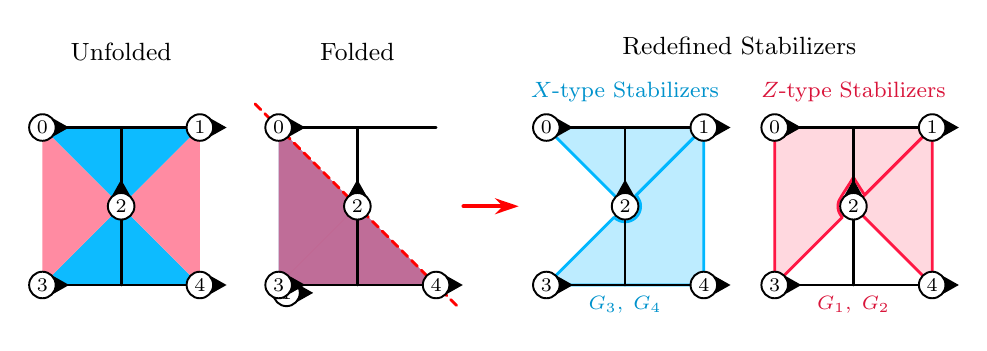
\begin{tikzpicture}[line cap=round,line join=round,thick,scale=1.0]
  \coordinate (Left)   at (-4.85, 0);
  \coordinate (Middle) at (-1.85, 0);
  \coordinate (XGrid)  at ( 1.55, 0);
  \coordinate (ZGrid)  at ( 4.45, 0);

  \node[above,font=\small] at ($(Left)+(0,1.72)$) {Unfolded};
  \node[above,font=\small] at ($(Middle)+(0,1.72)$) {Folded};
  \node[above,font=\small] at ($(XGrid)!0.5!(ZGrid)+(0,1.80)$) {Redefined Stabilizers};
  \node[above,font=\footnotesize,text=Xcol!80!black] at ($(XGrid)+(0,1.20)$) {$X$-type Stabilizers};
  \node[above,font=\footnotesize,text=Zcol!85!black] at ($(ZGrid)+(0,1.20)$) {$Z$-type Stabilizers};
  \node[font=\scriptsize,text=Xcol!80!black] at ($(XGrid)+(0,-1.25)$) {$G_3,\;G_4$};
  \node[font=\scriptsize,text=Zcol!85!black] at ($(ZGrid)+(0,-1.25)$) {$G_1,\;G_2$};

  % --- Left Patch (Unfolded) ---
  \begin{scope}[shift={(Left)}]
    \FiveQPatchFilled
    \FiveQPatchCircles
  \end{scope}

  % --- Middle Patch (Folded) ---
  \begin{scope}[shift={(Middle)}]
    \FiveQPatchOverlapped
    \def\m{0.30}
    \draw[dashed, draw=red, line width=1pt, dash pattern=on 3pt off 2pt]
      ($(q0)+(-\m,\m)$) -- ($(q4)+(\m,-\m)$);
    \FiveQPatchCirclesOneUnderThree
  \end{scope}

  \draw[-{Stealth[length=3mm,width=2mm]},red,line width=1.6pt]
    ($(Middle)+(1.35,0)$) -- ($(XGrid)+(-1.35,0)$);

  % --- Redefined X-type grid ---
  \begin{scope}[shift={(XGrid)}]
    \FiveQPatchRedefinedXGrid
    \FiveQPatchCircles
  \end{scope}

  % --- Redefined Z-type grid ---
  \begin{scope}[shift={(ZGrid)}]
    \FiveQPatchRedefinedZGrid
    \FiveQPatchCircles
  \end{scope}
\end{tikzpicture}
\caption{Five-qutrit patch}
\end{subfigure}

\vspace{2.0ex}

% ===================== (b) Definition =====================
\hspace*{-1.5em}
\begin{subfigure}[c]{0.48\textwidth}
\centering
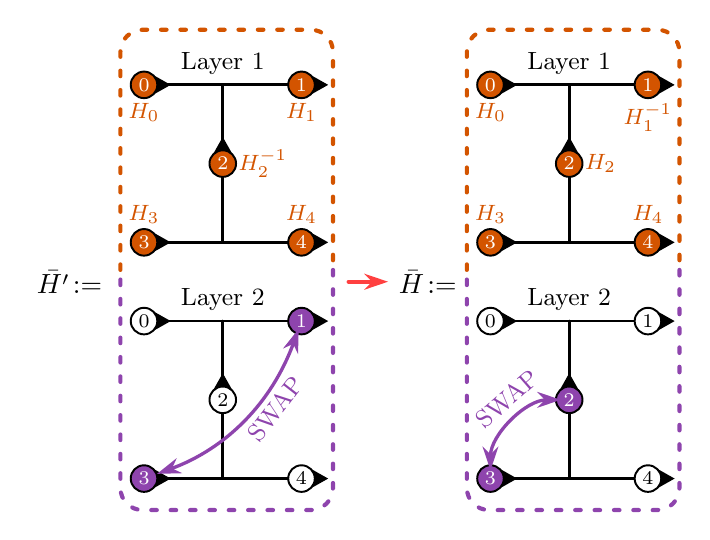
\begin{tikzpicture}[line cap=round,line join=round,thick,scale=1.0]
  \coordinate (LeftTop) at (-2.2,  1.50);
  \coordinate (LeftBot) at (-2.2, -1.50);
  \coordinate (RightTop) at ( 2.2,  1.50);
  \coordinate (RightBot) at ( 2.2, -1.50);

  \node[scale=1.0, anchor=east] at ($(LeftTop)+(-1.4, -1.5)$) {$\bar{H'}\!:=$};
  \node[scale=1.0, anchor=east] (HLabel) at ($(RightTop)+(-1.3, -1.5)$) {$\bar{H}\!:=$};

  \def\lw{1.5pt} \def\rc{8pt}
  % LEFT BOX 
  \path let \p1 = ($(LeftTop)+(-1.3,1.7)$), \p2 = ($(LeftBot)+(1.4,-1.4)$)
        in coordinate (LTL) at (\x1,\y1) coordinate (LBR) at (\x2,\y2)
           coordinate (LTR) at (\x2,\y1) coordinate (LBL) at (\x1,\y2);
  \coordinate (LMidLeft) at ($(LTL)!0.5!(LBL)$); \coordinate (LMidRight) at ($(LTR)!0.5!(LBR)$);
  \draw[HCol, dash pattern=on 2pt off 5pt, line width=\lw, rounded corners=\rc] (LMidLeft)--(LTL)--(LTR)--(LMidRight);
  \draw[SwapCol, dash pattern=on 2pt off 5pt, line width=\lw, rounded corners=\rc] (LMidRight)--(LBR)--(LBL)--(LMidLeft);

  % RIGHT BOX
  \path let \p1 = ($(RightTop)+(-1.3,1.7)$), \p2 = ($(RightBot)+(1.4,-1.4)$)
        in coordinate (RTL) at (\x1,\y1) coordinate (RBR) at (\x2,\y2)
           coordinate (RTR) at (\x2,\y1) coordinate (RBL) at (\x1,\y2);
  \coordinate (RMidLeft) at ($(RTL)!0.5!(RBL)$); \coordinate (RMidRight) at ($(RTR)!0.5!(RBR)$);
  \draw[HCol, dash pattern=on 2pt off 5pt, line width=\lw, rounded corners=\rc] (RMidLeft)--(RTL)--(RTR)--(RMidRight);
  \draw[SwapCol, dash pattern=on 2pt off 5pt, line width=\lw, rounded corners=\rc] (RMidRight)--(RBR)--(RBL)--(RMidLeft);

  \begin{scope}[shift={(LeftTop)}]
    \FiveQPatchEdges
    \foreach \P/\txt in {q0/0,q1/1,q2/2,q3/3,q4/4}{ \draw[line width=\qdLine,fill=HCol] (\P) circle (\qdR); \node[font=\numFont, text=white] at (\P) {\txt}; }
    \WedgeArrow{q0}{0}\WedgeArrow{q1}{0}\WedgeArrow{q3}{0}\WedgeArrow{q4}{0}\WedgeArrow{q2}{90}
    \node[anchor=south, font=\small, yshift=0mm] at (0, 1.0) {Layer 1};
    \begin{scope}[text=HCol, font=\footnotesize]
       \node[below, yshift=-3pt] at (q0) {$H_0$}; \node[below, yshift=-3pt] at (q1) {$H_1$};
       \node[right, xshift=2pt]  at (q2) {$H_2^{-1}$}; \node[above, yshift=3pt]  at (q3) {$H_3$}; \node[above, yshift=3pt]  at (q4) {$H_4$};
    \end{scope}
  \end{scope}

  \begin{scope}[shift={(LeftBot)}]
    \FiveQPatchEdges
    \foreach \P/\txt in {q0/0,q2/2,q4/4}{ \draw[line width=\qdLine,fill=white] (\P) circle (\qdR); \node[font=\numFont] at (\P) {\txt}; }
    \foreach \P/\txt in {q1/1,q3/3}{ \draw[line width=\qdLine,fill=SwapCol] (\P) circle (\qdR); \node[font=\numFont, text=white] at (\P) {\txt}; }
    \WedgeArrow{q0}{0}\WedgeArrow{q1}{0}\WedgeArrow{q3}{0}\WedgeArrow{q4}{0}\WedgeArrow{q2}{90}
    \node[anchor=south, font=\small, yshift=0mm] at (0, 1.0) {Layer 2};
    \draw[{Stealth[length=3mm,width=2mm]}-{Stealth[length=3mm,width=2mm]}, color=SwapCol, line width=1.2pt, shorten >=5pt, shorten <=3pt]
      (q1) to[bend left=25] node[midway, below right, rotate=52, xshift=-7pt, font=\small] {SWAP} (q3);
  \end{scope}

  \draw[-{Stealth[length=3mm,width=2mm]},red!75,line width=1.6pt] (-0.6, 0) -- (-0.1, 0);

  \begin{scope}[shift={(RightTop)}]
    \FiveQPatchEdges
    \foreach \P/\txt in {q0/0,q1/1,q2/2,q3/3,q4/4}{ \draw[line width=\qdLine,fill=HCol] (\P) circle (\qdR); \node[font=\numFont, text=white] at (\P) {\txt}; }
    \WedgeArrow{q0}{0}\WedgeArrow{q1}{0}\WedgeArrow{q3}{0}\WedgeArrow{q4}{0}\WedgeArrow{q2}{90}
    \node[anchor=south, font=\small, yshift=0mm] at (0, 1.0) {Layer 1};
    \begin{scope}[text=HCol, font=\footnotesize]
       \node[below, yshift=-3pt] at (q0) {$H_0$}; \node[below, yshift=-3pt] at (q1) {$H_1^{-1}$};
       \node[right, xshift=2pt]  at (q2) {$H_2$}; \node[above, yshift=3pt]  at (q3) {$H_3$}; \node[above, yshift=3pt]  at (q4) {$H_4$};
    \end{scope}
  \end{scope}

  \begin{scope}[shift={(RightBot)}]
    \FiveQPatchEdges
    \foreach \P/\txt in {q0/0,q1/1,q4/4}{ \draw[line width=\qdLine,fill=white] (\P) circle (\qdR); \node[font=\numFont] at (\P) {\txt}; }
    \foreach \P/\txt in {q2/2,q3/3}{ \draw[line width=\qdLine,fill=SwapCol] (\P) circle (\qdR); \node[font=\numFont, text=white] at (\P) {\txt}; }
    \WedgeArrow{q0}{0}\WedgeArrow{q1}{0}\WedgeArrow{q3}{0}\WedgeArrow{q4}{0}\WedgeArrow{q2}{90}
    \node[anchor=south, font=\small, yshift=0mm] at (0, 1.0) {Layer 2};
    \draw[{Stealth[length=3mm,width=2mm]}-{Stealth[length=3mm,width=2mm]}, color=SwapCol, line width=1.2pt, shorten >=3pt, shorten <=3pt]
      (q2) to[bend right=45] node[midway, below, xshift =-7pt, yshift=14pt, rotate=41, font=\small] {SWAP} (q3);
  \end{scope}
\end{tikzpicture}
\caption{Logical $\bar H$}
\label{fig: logical H}
\end{subfigure}
\quad
% ===================== (c) S Definition =====================
\begin{subfigure}[c]{0.48\textwidth}
\centering
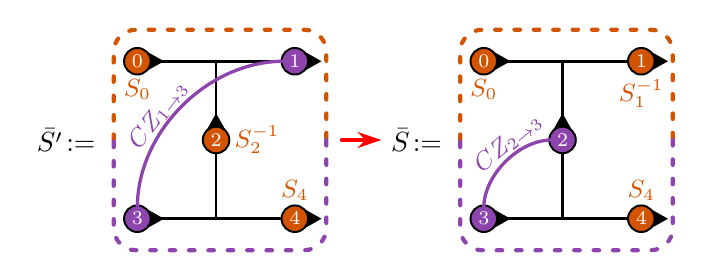
\begin{tikzpicture}[line cap=round,line join=round,thick,scale=1.0]
  \coordinate (Left)  at (-2.2, 0);
  \coordinate (Right) at ( 2.2, 0);
  \def\lw{1.5pt} \def\rc{8pt}

  \coordinate (LTL) at ($(Left)+(-1.3, 1.4)$); \coordinate (LBR) at ($(Left)+(1.4, -1.4)$);
  \coordinate (LTR) at ($(Left)+(1.4, 1.4)$);  \coordinate (LBL) at ($(Left)+(-1.3, -1.4)$);
  \coordinate (LMidLeft) at ($(LTL)!0.5!(LBL)$); \coordinate (LMidRight) at ($(LTR)!0.5!(LBR)$);
  \draw[HCol, dash pattern=on 2pt off 5pt, line width=\lw, rounded corners=\rc] (LMidLeft)--(LTL)--(LTR)--(LMidRight);
  \draw[SwapCol, dash pattern=on 2pt off 5pt, line width=\lw, rounded corners=\rc] (LMidRight)--(LBR)--(LBL)--(LMidLeft);

  \coordinate (RTL) at ($(Right)+(-1.3, 1.4)$); \coordinate (RBR) at ($(Right)+(1.4, -1.4)$);
  \coordinate (RTR) at ($(Right)+(1.4, 1.4)$);  \coordinate (RBL) at ($(Right)+(-1.3, -1.4)$);
  \coordinate (RMidLeft) at ($(RTL)!0.5!(RBL)$); \coordinate (RMidRight) at ($(RTR)!0.5!(RBR)$);
  \draw[HCol, dash pattern=on 2pt off 5pt, line width=\lw, rounded corners=\rc] (RMidLeft)--(RTL)--(RTR)--(RMidRight);
  \draw[SwapCol, dash pattern=on 2pt off 5pt, line width=\lw, rounded corners=\rc] (RMidRight)--(RBR)--(RBL)--(RMidLeft);

  \node[scale=1.0, anchor=east] at ($(Left)+(-1.4, 0)$) {$\bar{S'}\!:=$};
  \node[scale=1.0, anchor=east] (SLabel) at ($(Right)+(-1.4, 0)$) {$\bar{S}\!:=$};

  \newcommand{\DrawLHSPattern}{
      \FiveQPatchEdges
      \foreach \P in {q0, q2, q4} { \draw[line width=\qdLine,fill=HCol] (\P) circle (\qdR); }
      \foreach \P in {q1, q3} { \draw[line width=\qdLine,fill=SwapCol] (\P) circle (\qdR); }
      \foreach \P/\txt in {q0/0,q1/1,q2/2,q3/3,q4/4}{ \node[font=\numFont, text=white] at (\P) {\txt}; }
      \WedgeArrow{q0}{0}\WedgeArrow{q1}{0}\WedgeArrow{q3}{0}\WedgeArrow{q4}{0}\WedgeArrow{q2}{90}
      \node[text=HCol, font=\small, below, yshift=-3pt] at (q0) {$S_0$};
      \node[text=HCol, font=\small, right, xshift=3pt] at (q2) {$S_2^{-1}$};
      \node[text=HCol, font=\small, above, yshift=3pt] at (q4) {$S_4$};
      \draw[color=SwapCol, line width=1.2pt, shorten <=4pt, shorten >=4pt] 
         (q1) to[out=180, in=90] coordinate[pos=0.45] (mid) (q3);
      \node[text=SwapCol, font=\small, rotate=52, anchor=south, xshift=-12pt, yshift=-1pt] at (mid) {$CZ_{1\to 3}$};
  }
  \newcommand{\DrawRHSPattern}{
      \FiveQPatchEdges
      \foreach \P in {q0, q1, q4} { \draw[line width=\qdLine,fill=HCol] (\P) circle (\qdR); }
      \foreach \P in {q2, q3} { \draw[line width=\qdLine,fill=SwapCol] (\P) circle (\qdR); }
      \foreach \P/\txt in {q0/0,q1/1,q2/2,q3/3,q4/4}{ \node[font=\numFont, text=white] at (\P) {\txt}; }
      \WedgeArrow{q0}{0}\WedgeArrow{q1}{0}\WedgeArrow{q3}{0}\WedgeArrow{q4}{0}\WedgeArrow{q2}{90}
      \node[text=HCol, font=\small, below, yshift=-3pt] at (q0) {$S_0$};
      \node[text=HCol, font=\small, below, yshift=-3pt] at (q1) {$S_1^{-1}$};
      \node[text=HCol, font=\small, above, yshift=3pt] at (q4) {$S_4$};
      \draw[color=SwapCol, line width=1.2pt, shorten <=4pt, shorten >=4pt] 
         (q3) to[out=90, in=180] coordinate[pos=0.5] (midR) (q2);
      \node[text=SwapCol, font=\small, rotate=40, anchor=south, xshift=5pt, yshift=-2pt] at (midR) {$CZ_{2\to 3}$};
  }
  \begin{scope}[shift={(Left)}] \DrawLHSPattern \end{scope}
  \begin{scope}[shift={(Right)}] \DrawRHSPattern \end{scope}
  \draw[-{Stealth[length=3mm,width=2mm]},red,line width=1.6pt] (-0.6, 0) -- (-0.1, 0);
\end{tikzpicture}
\caption{Logical $\bar S$}
\label{fig: logical S}
\end{subfigure}

\vspace{2.0ex}

% ===================== (d) Parallel Operations =====================
\begin{subfigure}[b]{0.9\textwidth}
\centering
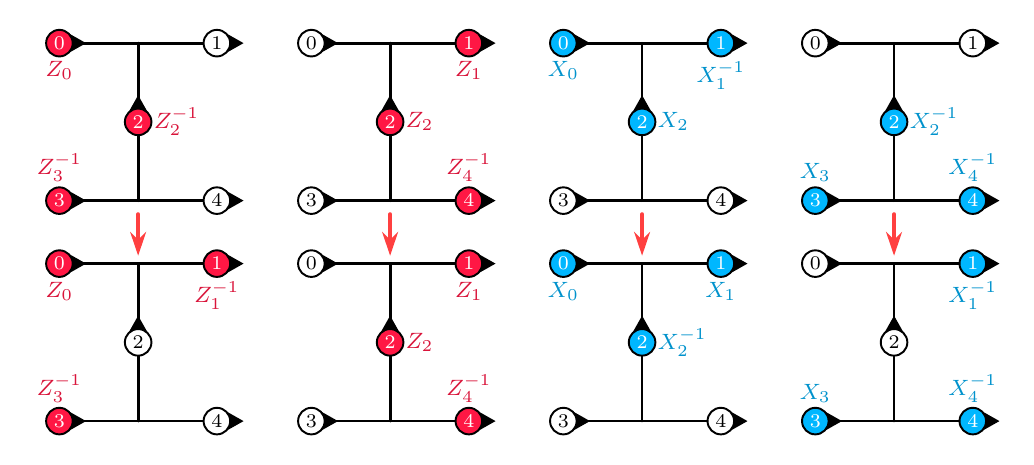
\begin{tikzpicture}[line cap=round,line join=round,thick,scale=1.0]
  \def\yTop{1.6} \def\yBot{-1.2}

  % COL 1
  \def\x{-4.8}
  \begin{scope}[shift={(\x, \yTop)}]
     \FiveQPatchEdges
     \foreach \P/\txt in {q1/1, q4/4}{ \draw[line width=\qdLine,fill=white] (\P) circle (\qdR); \node[font=\numFont] at (\P) {\txt}; }
     \foreach \P/\txt in {q0/0, q2/2, q3/3}{ \draw[line width=\qdLine,fill=Zcol] (\P) circle (\qdR); \node[font=\numFont, text=white] at (\P) {\txt}; }
     \WedgeArrow{q0}{0}\WedgeArrow{q1}{0}\WedgeArrow{q3}{0}\WedgeArrow{q4}{0}\WedgeArrow{q2}{90}
     \begin{scope}[text=Zcol!85!black, font=\footnotesize]
        \node[below, yshift=-3pt] at (q0) {$Z_0$}; \node[right, xshift=2pt] at (q2) {$Z_2^{-1}$}; \node[above, yshift=3pt] at (q3) {$Z_3^{-1}$};
     \end{scope}
  \end{scope}
  \begin{scope}[shift={(\x, \yBot)}]
     \FiveQPatchEdges
     \foreach \P/\txt in {q2/2, q4/4}{ \draw[line width=\qdLine,fill=white] (\P) circle (\qdR); \node[font=\numFont] at (\P) {\txt}; }
     \foreach \P/\txt in {q0/0, q1/1, q3/3}{ \draw[line width=\qdLine,fill=Zcol] (\P) circle (\qdR); \node[font=\numFont, text=white] at (\P) {\txt}; }
     \WedgeArrow{q0}{0}\WedgeArrow{q1}{0}\WedgeArrow{q3}{0}\WedgeArrow{q4}{0}\WedgeArrow{q2}{90}
     \begin{scope}[text=Zcol!85!black, font=\footnotesize]
        \node[below, yshift=-3pt] at (q0) {$Z_0$}; \node[below, yshift=-3pt] at (q1) {$Z_1^{-1}$}; \node[above, yshift=3pt] at (q3) {$Z_3^{-1}$};
     \end{scope}
  \end{scope}
  \draw[-{Stealth[length=3mm,width=2mm]},red!75,line width=1.6pt] (\x, 0.425) -- (\x, -0.1);

  % COL 2
  \def\x{-1.6}
  \begin{scope}[shift={(\x, \yTop)}]
     \FiveQPatchEdges
     \foreach \P/\txt in {q0/0, q3/3}{ \draw[line width=\qdLine,fill=white] (\P) circle (\qdR); \node[font=\numFont] at (\P) {\txt}; }
     \foreach \P/\txt in {q1/1, q2/2, q4/4}{ \draw[line width=\qdLine,fill=Zcol] (\P) circle (\qdR); \node[font=\numFont, text=white] at (\P) {\txt}; }
     \WedgeArrow{q0}{0}\WedgeArrow{q1}{0}\WedgeArrow{q3}{0}\WedgeArrow{q4}{0}\WedgeArrow{q2}{90}
     \begin{scope}[text=Zcol!85!black, font=\footnotesize]
        \node[below, yshift=-3pt] at (q1) {$Z_1$}; \node[right, xshift=2pt] at (q2) {$Z_2$}; \node[above, yshift=3pt] at (q4) {$Z_4^{-1}$};
     \end{scope}
  \end{scope}
  \begin{scope}[shift={(\x, \yBot)}]
     \FiveQPatchEdges
     \foreach \P/\txt in {q0/0, q3/3}{ \draw[line width=\qdLine,fill=white] (\P) circle (\qdR); \node[font=\numFont] at (\P) {\txt}; }
     \foreach \P/\txt in {q1/1, q2/2, q4/4}{ \draw[line width=\qdLine,fill=Zcol] (\P) circle (\qdR); \node[font=\numFont, text=white] at (\P) {\txt}; }
     \WedgeArrow{q0}{0}\WedgeArrow{q1}{0}\WedgeArrow{q3}{0}\WedgeArrow{q4}{0}\WedgeArrow{q2}{90}
     \begin{scope}[text=Zcol!85!black, font=\footnotesize]
        \node[below, yshift=-3pt] at (q1) {$Z_1$}; \node[right, xshift=2pt] at (q2) {$Z_2$}; \node[above, yshift=3pt] at (q4) {$Z_4^{-1}$};
     \end{scope}
  \end{scope}
  \draw[-{Stealth[length=3mm,width=2mm]},red!75,line width=1.6pt] (\x, 0.425) -- (\x, -0.1);

  % COL 3
  \def\x{1.6}
  \begin{scope}[shift={(\x, \yTop)}]
     \FiveQPatchEdges
     \foreach \P/\txt in {q3/3, q4/4}{ \draw[line width=\qdLine,fill=white] (\P) circle (\qdR); \node[font=\numFont] at (\P) {\txt}; }
     \foreach \P/\txt in {q0/0, q1/1, q2/2}{ \draw[line width=\qdLine,fill=Xcol] (\P) circle (\qdR); \node[font=\numFont, text=white] at (\P) {\txt}; }
     \WedgeArrow{q0}{0}\WedgeArrow{q1}{0}\WedgeArrow{q3}{0}\WedgeArrow{q4}{0}\WedgeArrow{q2}{90}
     \begin{scope}[text=Xcol!80!black, font=\footnotesize]
        \node[below, yshift=-3pt] at (q0) {$X_0$}; \node[below, yshift=-3pt] at (q1) {$X_1^{-1}$}; \node[right, xshift=2pt] at (q2) {$X_2$};
     \end{scope}
  \end{scope}
  \begin{scope}[shift={(\x, \yBot)}]
     \FiveQPatchEdges
     \foreach \P/\txt in {q3/3, q4/4}{ \draw[line width=\qdLine,fill=white] (\P) circle (\qdR); \node[font=\numFont] at (\P) {\txt}; }
     \foreach \P/\txt in {q0/0, q1/1, q2/2}{ \draw[line width=\qdLine,fill=Xcol] (\P) circle (\qdR); \node[font=\numFont, text=white] at (\P) {\txt}; }
     \WedgeArrow{q0}{0}\WedgeArrow{q1}{0}\WedgeArrow{q3}{0}\WedgeArrow{q4}{0}\WedgeArrow{q2}{90}
     \begin{scope}[text=Xcol!80!black, font=\footnotesize]
        \node[below, yshift=-3pt] at (q0) {$X_0$}; \node[below, yshift=-3pt] at (q1) {$X_1$}; \node[right, xshift=2pt] at (q2) {$X_2^{-1}$};
     \end{scope}
  \end{scope}
  \draw[-{Stealth[length=3mm,width=2mm]},red!75,line width=1.6pt] (\x, 0.425) -- (\x, -0.1);

  % COL 4
  \def\x{4.8}
  \begin{scope}[shift={(\x, \yTop)}]
     \FiveQPatchEdges
     \foreach \P/\txt in {q0/0, q1/1}{ \draw[line width=\qdLine,fill=white] (\P) circle (\qdR); \node[font=\numFont] at (\P) {\txt}; }
     \foreach \P/\txt in {q2/2, q3/3, q4/4}{ \draw[line width=\qdLine,fill=Xcol] (\P) circle (\qdR); \node[font=\numFont, text=white] at (\P) {\txt}; }
     \WedgeArrow{q0}{0}\WedgeArrow{q1}{0}\WedgeArrow{q3}{0}\WedgeArrow{q4}{0}\WedgeArrow{q2}{90}
     \begin{scope}[text=Xcol!80!black, font=\footnotesize]
        \node[right, xshift=2pt] at (q2) {$X_2^{-1}$}; \node[above, yshift=3pt] at (q3) {$X_3$}; \node[above, yshift=3pt] at (q4) {$X_4^{-1}$};
     \end{scope}
  \end{scope}
  \begin{scope}[shift={(\x, \yBot)}]
     \FiveQPatchEdges
     \foreach \P/\txt in {q0/0, q2/2}{ \draw[line width=\qdLine,fill=white] (\P) circle (\qdR); \node[font=\numFont] at (\P) {\txt}; }
     \foreach \P/\txt in {q1/1, q3/3, q4/4}{ \draw[line width=\qdLine,fill=Xcol] (\P) circle (\qdR); \node[font=\numFont, text=white] at (\P) {\txt}; }
     \WedgeArrow{q0}{0}\WedgeArrow{q1}{0}\WedgeArrow{q3}{0}\WedgeArrow{q4}{0}\WedgeArrow{q2}{90}
     \begin{scope}[text=Xcol!80!black, font=\footnotesize]
        \node[below, yshift=-3pt] at (q1) {$X_1^{-1}$}; \node[above, yshift=3pt] at (q3) {$X_3$}; \node[above, yshift=3pt] at (q4) {$X_4^{-1}$};
     \end{scope}
  \end{scope}
  \draw[-{Stealth[length=3mm,width=2mm]},red!75,line width=1.6pt] (\x, 0.425) -- (\x, -0.1);
\end{tikzpicture}
\caption{Stabilizer generators}
\end{subfigure}

\vspace{2.0ex}
% ===================== (e) Logical X =====================
\begin{subfigure}[c]{0.35\textwidth}
\centering
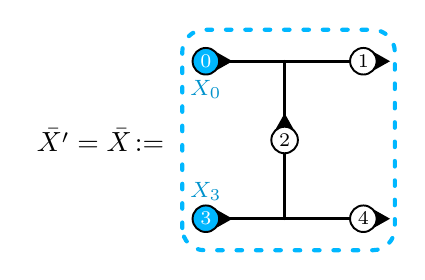
\begin{tikzpicture}[line cap=round,line join=round,thick,scale=1.0]
  \node[scale=1.0, anchor=east] at (-1.4, 0) {$\bar{X'}=\bar{X}\!:=$};
   
  % Added blue box
  \def\lw{1.5pt} \def\rc{8pt}
  \coordinate (LTL_X) at (-1.3, 1.4); \coordinate (LBR_X) at (1.4, -1.4);
  \coordinate (LTR_X) at ( 1.4, 1.4); \coordinate (LBL_X) at (-1.3, -1.4);
  \draw[Xcol, dash pattern=on 2pt off 5pt, line width=\lw, rounded corners=\rc] (LBL_X)--(LTL_X)--(LTR_X)--(LBR_X)--cycle;
   
  \FiveQPatchEdges
  \foreach \P/\txt in {q1/1, q2/2, q4/4}{ \draw[line width=\qdLine,fill=white] (\P) circle (\qdR); \node[font=\numFont] at (\P) {\txt}; }
  \foreach \P/\txt in {q0/0, q3/3}{ \draw[line width=\qdLine,fill=Xcol] (\P) circle (\qdR); \node[font=\numFont, text=white] at (\P) {\txt}; }
  \WedgeArrow{q0}{0}\WedgeArrow{q1}{0}\WedgeArrow{q3}{0}\WedgeArrow{q4}{0}\WedgeArrow{q2}{90}
  \begin{scope}[text=Xcol!80!black, font=\footnotesize]
     \node[below, yshift=-3pt] at (q0) {$X_0$};
     \node[above, yshift=3pt]  at (q3) {$X_3$};
  \end{scope}
\end{tikzpicture}
\caption{Logical $\bar X$}
\end{subfigure}
\quad
% ===================== (f) Logical Z =====================
\begin{subfigure}[c]{0.6\textwidth}
\centering
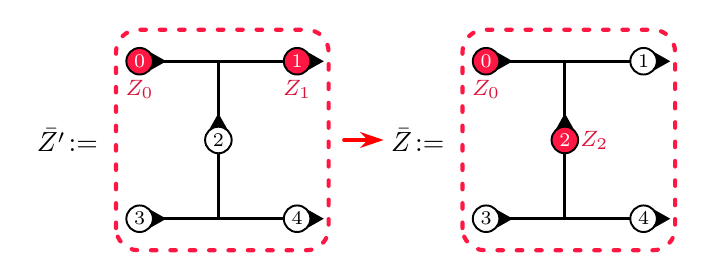
\begin{tikzpicture}[line cap=round,line join=round,thick,scale=1.0]
  % Define centers
  \coordinate (Left)  at (-2.2, 0);
  \coordinate (Right) at ( 2.2, 0);

  % Labels
  \node[scale=1.0, anchor=east] at ($(Left)+(-1.4, 0)$) {$\bar{Z'}\!:=$};
  \node[scale=1.0, anchor=east] at ($(Right)+(-1.4, 0)$) {$\bar{Z}\!:=$};
   
  % Added red boxes
  \def\lw{1.5pt} \def\rc{8pt}
  % Left Box
  \coordinate (LTL_Z) at ($(Left)+(-1.3, 1.4)$); \coordinate (LBR_Z) at ($(Left)+(1.4, -1.4)$);
  \coordinate (LTR_Z) at ($(Left)+(1.4, 1.4)$); \coordinate (LBL_Z) at ($(Left)+(-1.3, -1.4)$);
  \draw[Zcol, dash pattern=on 2pt off 5pt, line width=\lw, rounded corners=\rc] (LBL_Z)--(LTL_Z)--(LTR_Z)--(LBR_Z)--cycle;

  % Right Box
  \coordinate (RTL_Z) at ($(Right)+(-1.3, 1.4)$); \coordinate (RBR_Z) at ($(Right)+(1.4, -1.4)$);
  \coordinate (RTR_Z) at ($(Right)+(1.4, 1.4)$); \coordinate (RBL_Z) at ($(Right)+(-1.3, -1.4)$);
  \draw[Zcol, dash pattern=on 2pt off 5pt, line width=\lw, rounded corners=\rc] (RBL_Z)--(RTL_Z)--(RTR_Z)--(RBR_Z)--cycle;

  % Left Patch: Z0 Z1
  \begin{scope}[shift={(Left)}]
     \FiveQPatchEdges
     \foreach \P/\txt in {q2/2, q3/3, q4/4}{ \draw[line width=\qdLine,fill=white] (\P) circle (\qdR); \node[font=\numFont] at (\P) {\txt}; }
     \foreach \P/\txt in {q0/0, q1/1}{ \draw[line width=\qdLine,fill=Zcol] (\P) circle (\qdR); \node[font=\numFont, text=white] at (\P) {\txt}; }
     \WedgeArrow{q0}{0}\WedgeArrow{q1}{0}\WedgeArrow{q3}{0}\WedgeArrow{q4}{0}\WedgeArrow{q2}{90}
     \begin{scope}[text=Zcol!85!black, font=\footnotesize]
        \node[below, yshift=-3pt] at (q0) {$Z_0$};
        \node[below, yshift=-3pt] at (q1) {$Z_1$};
     \end{scope}
  \end{scope}

  % Right Patch: Z0 Z2
  \begin{scope}[shift={(Right)}]
     \FiveQPatchEdges
     \foreach \P/\txt in {q1/1, q3/3, q4/4}{ \draw[line width=\qdLine,fill=white] (\P) circle (\qdR); \node[font=\numFont] at (\P) {\txt}; }
     \foreach \P/\txt in {q0/0, q2/2}{ \draw[line width=\qdLine,fill=Zcol] (\P) circle (\qdR); \node[font=\numFont, text=white] at (\P) {\txt}; }
     \WedgeArrow{q0}{0}\WedgeArrow{q1}{0}\WedgeArrow{q3}{0}\WedgeArrow{q4}{0}\WedgeArrow{q2}{90}
     \begin{scope}[text=Zcol!85!black, font=\footnotesize]
        \node[below, yshift=-3pt] at (q0) {$Z_0$};
        \node[right, xshift=2pt]  at (q2) {$Z_2$};
     \end{scope}
  \end{scope}

  % Arrow in middle (adjusted for gap)
  \draw[-{Stealth[length=3mm,width=2mm]},red,line width=1.6pt] (-0.6, 0) -- (-0.1, 0);

\end{tikzpicture}
\caption{Logical $\bar Z$}
\end{subfigure}
% END OF PAGE 1
\end{figure*}

\begin{figure*}[tp]\ContinuedFloat
\centering
% ===== MAIN CAPTION HERE =====
% Caption shortened and scoped to the patch with q2 at the center (track hw, 2026-11-13). The former caption is in paper-rework/draft/.
\caption{The $[[5,1,2]]_3$ code on the patch with $q_2$ at the center. Primed symbols are the definitions of the folded-code construction~\cite{Moussa2016}, and unprimed symbols are ours, which exchange the roles of $q_1$ and $q_2$. Blue marks $X$-type and red $Z$-type operators; in (b) and (c), orange marks one-qutrit gates and purple the two-qutrit gate. The wedge on a qutrit points along its edge of the surface-code lattice (\appref{app:background}).
(a)~The patch of the folded-code construction, unfolded and folded, and our stabilizers.
(b)~Logical Hadamard gate: a layer of one-qutrit gates (Layer~1) and one SWAP gate (Layer~2), between the opposite corners $q_1$ and $q_3$ in $\bar H'$ and between the diagonal neighbors $q_2$ and $q_3$ in $\bar H$.
(c)~Logical phase gate, with its CZ gate on $q_1$ and $q_3$ in $\bar S'$ and on $q_2$ and $q_3$ in $\bar S$.
(d)~Stabilizer generators of the folded-code construction (top row) and ours (bottom row), $G_1$ to $G_4$ from left to right.
(e)~Logical $\bar X$, the same in both.
(f)~Logical $\bar Z' = Z_0 Z_1$ and $\bar Z = Z_0 Z_2$.}
\label{fig: 5-qutrit-code}

\end{figure*}



\section{Logical Randomized Benchmarking with Detection}
\label{sub:lrb_d}\label{subsub:postselection}

% Sec. III of the restructured sim version (style: jpw-review/sim/style-snap.md). Rewritten 2026-11-20 (user): LRB-D as a protocol for any stabilizer code, with its steps as a numbered list (D1-D7); the steps of RB and LRB stay in Appendix A as lists; a subsection "What LRB-D measures" states the properties of the protocol once, including the cost in shots, and ends on the hardware each variant needs. Outline: jpw-review/sim/outline-III-v2.md. Moved out of the main text: the weight of a depth with zero spread and the parametric bootstrap (Appendix C); the statement that the baseline's only channel is DEP1 and that its readout is noiseless (Sec. V, noise models).
% Novelty statement from the literature search of 2026-11-20 (jpw-review/sim/lit-search-lrbd.md): the name LRB-D and its terminal-check form are in the sdim paper (arXiv:2511.12777, Sec. VII, gate-level depolarizing noise, no pseudo-threshold); postselected logical RB of a distance-two code with a final parity check is Harper & Flammia 2019; a fixed detection cadence in logical cycle benchmarking is Dasu et al. 2026. Do not call LRB-D new.
Logical randomized benchmarking with detection (LRB-D) adapts logical randomized benchmarking~\cite{Combes2017} to error detection. Logical randomized benchmarking corrects errors after each logical gate and therefore needs a distance of at least three (\appref{app:background-lrb}); LRB-D keeps the syndrome measurements and replaces the correction by postselection. Reference~\cite{sdim} introduced LRB-D for the $[[5,1,2]]_3$ code with a single check round at the end of the circuit and depolarizing noise after each logical Clifford. Harper and Flammia~\cite{Harper2019FTIBM} postselected logical randomized benchmarking of a distance-two qubit code on the final readout alone, Self \emph{et al.}~\cite{Self2024} compared encoded mirror circuits with zero to three syndrome rounds, and Dasu \emph{et al.}~\cite{Dasu2026} checked the syndromes at one fixed interval of logical cycle benchmarking. We extend LRB-D to a check round after every logical Clifford, with the rounds that enter the postselection chosen afterwards on the same shots, and to circuit-level noise, under which we compare it with a physical baseline (\autoref{sub:fit_model}).

\autoref{fig:lrb_overview} gives an overview of LRB-D. The remainder of this section is organized as follows. In \autoref{sub:lrbd_circuits} we give the steps of LRB-D, in \autoref{sub:postselection_schedules} the schedules that decide which syndromes enter the postselection, and in \autoref{sub:fit_model} how the accepted shots become an error rate and a pseudo-threshold. \autoref{sub:lrbd_measures} states what the protocol measures, what it costs in shots and what it needs from hardware.

\subsection{Protocol}
\label{sub:lrbd_circuits}

LRB-D needs three things of a code: stabilizer generators $G_1, \dots, G_{n_G}$ whose syndromes can be measured, a logical Pauli operator $\bar P$ whose eigenstate can be prepared and which can be measured, and circuits for the logical Clifford gates. Every stabilizer code of prime local dimension provides them, so LRB-D applies to every such code of distance at least two; for a code of larger distance, it benchmarks the code used as an error detector. For any stabilizer code of distance at least two, LRB-D of depth $m$ has seven steps. Steps~\ref{step:D1} to~\ref{step:D5} make up the circuit of \autoref{fig:lrb_overview}, and steps~\ref{step:D6} and~\ref{step:D7} act on its outcomes. For the $[[5,1,2]]_3$ code, $n_G = 4$ and $\bar P = \bar X$.
\begin{enumerate}[label=\textbf{D\arabic*.}, ref=D\arabic*, leftmargin=2.1em, labelsep=0.4em, itemsep=1pt, topsep=3pt]
  \item\label{step:D1} \textbf{Encoding.} Prepare the $+1$ eigenstate of $\bar P$. For the $[[5,1,2]]_3$ code, an encoding circuit (\autoref{fig:encoding_circuit}) prepares this state, $\ket{\bar{+}}$.
  \item\label{step:D2} \textbf{Random sequence with check rounds.} Apply $m$ logical Cliffords $\bar C_1$, \dots, $\bar C_m$, drawn independently and uniformly from the logical Clifford group, which for one qutrit has $216$ elements up to a global phase (\appref{sec:clifford-gen}). A check round $\mathcal{R}_t$ follows each $\bar C_t$: it resets the ancillas, maps the syndromes of $G_1, \dots, G_{n_G}$ onto them and reads them out.
  \item\label{step:D3} \textbf{Mirror inverse.} Apply $\bar C_m^{-1}, \dots, \bar C_1^{-1}$, one Clifford at a time as in mirror circuits~\cite{Proctor2022MirrorRB} and with no check round in between, which in the absence of errors returns the code to the state of step~\ref{step:D1}.
  \item\label{step:D4} \textbf{Final check round.} Apply a last check round $\mathcal{R}_{m+1}$.
  \item\label{step:D5} \textbf{Logical readout.} Measure $\bar P$. For the $[[5,1,2]]_3$ code we measure $q_0$ and $q_3$ in the $X$ basis, and the sum of the two outcomes modulo three, the outcome of $\bar X$ of Eq.~\eqref{eq:logicalPauli}, is the logical outcome, which is zero in the absence of errors.
  \item\label{step:D6} \textbf{Postselection.} Accept the shot if every syndrome of the check rounds that enter the postselection under the chosen schedule (\autoref{sub:postselection_schedules}) is trivial, and reject it otherwise.
  \item\label{step:D7} \textbf{Fit and comparison.} Repeat steps~\ref{step:D1} to~\ref{step:D6} for many shots of each of many random sequences at several depths $m$, fit the decay of the logical signal of the accepted shots with $m$, and compare the resulting error rate with that of a physical qudit (\autoref{sub:fit_model}).
\end{enumerate}
A unit of depth is thus a forward Clifford with its check round and its inverse, and a circuit of depth $m$ contains $2m$ logical Cliffords and $m+1$ check rounds. The check rounds depend on the connectivity of the device, and \autoref{sub:ancilla_layouts} gives them for two layouts of the $[[5,1,2]]_3$ code.

% TODO(sim): this figure becomes the overview figure of LRB-D (user, 2026-11-20): panel (a) a flowchart from encoding to the pseudo-threshold, drawn in TikZ by the figure session (brief: jpw-review/handoff/sim-overview-figure-brief.md); panel (b) this circuit. Until then the text cites the figure without panel letters.
\begin{figure*}[tp]
    \centering
        \scalebox{0.8}{
        \begin{quantikz}[row sep=0.45cm, column sep=0.22cm]
          \lstick{data $\ket{0}^{\otimes 5}$} & \qwbundle{5} &
            \gate{\textcolor{LightBlue}{U_{\mathrm{enc}}}} &
            \gate{\textcolor{red}{\bar C_t}}\gategroup[2,steps=4,style={dashed,rounded corners,inner xsep=2pt},background,label style={label position=below,anchor=north,yshift=-0.2cm}]{$t = 1, \dots, m$} &
            \gate[2]{\textcolor{purple}{\mathcal{N}}} &
            \gate[2]{\mathcal{R}_t} &
            \gate[2]{\textcolor{purple}{\mathcal{N}}} &
            &
            \gate{\textcolor{red}{\bar C_t^{-1}}}\gategroup[2,steps=2,style={dashed,rounded corners,inner xsep=2pt},background,label style={label position=below,anchor=north,yshift=-0.2cm}]{$t = m, \dots, 1$} &
            \gate[2]{\textcolor{purple}{\mathcal{N}}} &
            &
            \gate[2]{\mathcal{R}_{m+1}} &
            \gate[2]{\textcolor{purple}{\mathcal{N}}} &
            \meter{} & \rstick{$x_{\bar X}$} \\
          \lstick{ancillas $\ket{0}^{\otimes n_a}$} & \qwbundle{n_a} & & & & & & & & & & & & &
        \end{quantikz}
        }
    \caption{LRB-D circuit of depth $m$, steps~\ref{step:D1} to~\ref{step:D5}. The encoding circuit $U_{\mathrm{enc}}$ prepares $\ket{\bar +}$, the $+1$ eigenstate of $\bar X$, on the five data qutrits (\autoref{fig:encoding_circuit}). Each forward logical Clifford $\bar C_t$ is followed by a check round $\mathcal{R}_t$, which acts on the data qutrits and on the $n_a$ ancilla qutrits of the layout, four in the one-ancilla and two in the two-ancilla layout (\autoref{sub:ancilla_layouts}). The mirror inverse $\bar C_m^{-1}, \dots, \bar C_1^{-1}$ follows without check rounds, then the final check round $\mathcal{R}_{m+1}$ and the $X$-basis readout of $q_0$ and $q_3$, which gives the logical outcome $x_{\bar X}$. Each box $\mathcal{N}$ stands for the noise that the simulations attach to the preceding logical Clifford or check round (\autoref{sub:noise_models}).}
    \label{fig:lrb_d_full}\label{fig:lrb_a}\label{fig:lrb_overview}
\end{figure*}

\subsection{Postselection Schedules}
\label{sub:postselection_schedules}

Step~\ref{step:D6} leaves open which check rounds enter the postselection, and we vary this choice to learn how the error of the accepted shots depends on how often the syndromes are used. In uniform-interval postselection with interval $k$, every $k$-th of the rounds $\mathcal{R}_1, \dots, \mathcal{R}_m$ and the final round $\mathcal{R}_{m+1}$ enter the postselection, the rounds whose indices form the set
\begin{equation}
    \mathcal{T}_k(m) = \{\, k, 2k, \dots, \lfloor m/k \rfloor k \,\} \cup \{ m+1 \} .
    \label{eq:unif_rounds}
\end{equation}
For $k = 1$ every round is postselected, and for $m < k$ only the final one. The circuit executes all $m+1$ check rounds whatever the value of $k$, so all intervals share one set of circuits and shots and differ only in which shots they accept.

At the other extreme, terminal postselection measures no syndrome during the sequence: its circuits omit the check rounds of steps~\ref{step:D2} and~\ref{step:D4}, and step~\ref{step:D5} reads out every data qudit, so that only the stabilizers that this readout determines can be checked. For the $[[5,1,2]]_3$ code, all five data qutrits are measured in the $X$ basis, with outcomes $x_0, \dots, x_4$. These outcomes carry no information about the $Z$-type stabilizers, so only the two $X$-type stabilizers are checked: besides the logical outcome we evaluate $x_0 + x_1 - x_2$ for $G_3$ and $x_3 - x_1 - x_4$ for $G_4$ modulo three, and step~\ref{step:D6} accepts a shot if both values are zero.

\subsection{Error Rates and the Pseudo-Threshold}
\label{sub:fit_model}

To decide whether the encoding pays, we compare LRB-D with its physical baseline, randomized benchmarking (RB) of one physical qutrit, run under the same noise model (\appref{app:background-rb} gives its steps, its signal and its fit). Since its Cliffords are the words of the logical Cliffords, the comparison measures what the encoding, with its check rounds and its postselection, changes.

Both error rates come from signals built in the same way, which we give for LRB-D. For a sequence $s$ at depth $m$, let $P_j$ be the fraction of its accepted shots with logical outcome $j$. The complex estimate
\begin{equation}
    \langle \bar{X} \rangle_s = \sum_{j=0}^{2} \omega^{-j} P_j
    \label{eq:estimator}
\end{equation}
is an estimate of the expectation value of $\bar X$ in the accepted shots and is one if every accepted shot has the outcome zero. We take its modulus, average the modulus over the sequences, and call this average $\langle \bar{X} \rangle$ the accepted logical signal.

A fit over the depths turns the signal into an error rate per unit of depth. We fit the accepted logical signal, and the signal of the baseline in the same way, as a function of the depth with
\begin{equation}
    F(m) = A f^{m},
    \label{eq:zero_offset_fit}
\end{equation}
by weighted least squares with weights $1/\sigma_m^2$, where $\sigma_m$ is the standard deviation of the per-sequence moduli at depth $m$. The fit uses every depth at which every sequence has at least one accepted shot, $m = 0$ included (\autoref{sub:sim_framework} states one exception, and \appref{app:campaign} gives the weight of a depth with $\sigma_m = 0$). The model has no constant offset because, in the limit of many shots, the estimate of Eq.~\eqref{eq:estimator} has zero expectation for a fully depolarized qutrit. The modulus of a finite-shot estimate stays above zero, and \appref{app:campaign} gives this floor. Errors that do not depend on the depth, such as those of the final check round, enter the amplitude $A$. The decay parameter $f$ gives the average fidelity $\bar F$ and the error rate $r$ per unit of depth,
\begin{equation}
    \bar{F} = \frac{2f + 1}{3}, \qquad r = 1 - \bar{F} = \frac{2}{3}\,(1 - f) .
    \label{eq:error_rate}
\end{equation}
Equation~\eqref{eq:error_rate} has a simple reading. If the noise of one unit of depth, averaged over the random Cliffords, leaves the qutrit untouched with probability $f$ and depolarizes it otherwise, a depolarized qutrit still agrees with the ideal state with probability $1/3$, so the average fidelity is $f + (1-f)/3$ and the error rate is $\tfrac{2}{3}(1 - f)$.

% TODO(authors): which count should the main text lead with, 2542 (group generated by Hbar and Sbar, 216 elements up to phase) or 301 (group generated by Hbar, Sbar, Xbar and Zbar as simulated, 1944 elements)? Both are quoted until the coauthors decide (CONTRACT Amendment A3; jpw-review/OPEN-QUESTIONS.md, item 4). Verified by paper-rework/scratch/lead/irreps_check.py.
Unlike the decay of the baseline (\appref{app:background-rb}), the accepted decay need not be a single exponential~\cite{Ceasura2022}. The logical Cliffords twirl the noise on the operators of five qutrits, and the signal of a code state can depend on up to $2542$ eigenvalues for the group of five-qutrit unitaries generated by $\bar H$ and $\bar S$, and on up to $301$ for the larger group generated by the simulated gate set $\bar H$, $\bar S$, $\bar X$ and $\bar Z$ (\appref{sec:rep-theory}). We therefore quote the quality of every fit with more than two depths as $\chi^2$ per degree of freedom, $\chi^2/(n-2)$ with $\chi^2 = \sum_m (y_m - A f^m)^2/\sigma_m^2$ summed over the $n$ fitted depths, where $y_m$ is the signal at depth $m$, $\langle \bar X \rangle(m)$ for LRB-D. Because $\sigma_m$ is the standard deviation over the $N_s$ sequences of a run and not the standard error of their mean, $\sigma_m/\sqrt{N_s}$, residuals at the level of that standard error give a value of about $1/N_s$, not one.

With the two error rates in hand, we condense each combination of code, layout, noise model and interval $k$ into one number, the pseudo-threshold $p^\star(k)$: the value of the two-qutrit gate error probability $p$, the parameter that sets the strength of the noise (\autoref{sub:noise_models}), at which the error rate of LRB-D crosses that of the baseline under the same noise model. In every configuration we report, the logical qudit of the accepted shots has the lower error rate at every sampled $p > 0$ below $p^\star(k)$ and the higher one at every sampled $p$ above it. We obtain $p^\star(k)$ from a linear interpolation of the difference of the two error rates between the grid points on either side (\appref{app:campaign} gives the search rule and its tolerance). For the pseudo-thresholds, uncertainties are one standard error (68\% confidence), from a bootstrap over the random Clifford sequences. Each replicate resamples the sequences of every run that enters the pseudo-threshold, for LRB-D and for the baseline, refits all decays and repeats the search (\appref{app:campaign}).

\subsection{What LRB-D Measures}
\label{sub:lrbd_measures}

LRB-D returns two quantities for every depth: the distribution of the logical outcome over the accepted shots, from which step~\ref{step:D7} extracts an error rate per unit of depth for uniform-interval postselection (\autoref{sub:terminal_results} shows why terminal postselection gives none), and the fraction of shots that step~\ref{step:D6} rejects, the rejected fraction. The error rate describes the accepted shots only. It is therefore not the failure probability of a computation of depth $m$, which also counts the rejected shots, and we report the rejected fraction with it. Because all intervals share one set of shots (\autoref{sub:postselection_schedules}), the schedule can trade the two quantities against each other.

The price of postselection is paid in shots. Because the logical Cliffords map the stabilizer group to itself, a fault that leaves a detectable error on the data keeps the syndromes nontrivial until the next postselected round, whatever the interval, whereas a fault that corrupts only the syndrome readout of a round matters only if that round is postselected. Step~\ref{step:D6} therefore accepts a shot of depth $m$ with probability about
\begin{equation}
    e^{-\mu_d(m) - \mu_r\,|\mathcal{T}_k(m)|} ,
    \label{eq:acceptance}
\end{equation}
where $\mu_d(m)$, the expected number of faults in the circuit that leave a detectable error on the data, grows linearly with $m$ and increases with the size of the code and of its check rounds, and $\mu_r$, the expected number of faults per round that corrupt only its readout, grows with the number $n_G$ of syndromes that a round reads out. The accepted fraction thus falls exponentially with the depth at every interval we report, and postselecting more rounds of a code with more stabilizers lowers it further through the second term. Since a depth enters the fit only while every sequence has an accepted shot (\autoref{sub:fit_model}), the number of shots per sequence sets the largest depth that can be fitted, and this depth shrinks as $p$ grows; \autoref{sec:results} gives the rejected fractions of our runs.

The two kinds of postselection also ask different things of the hardware. Terminal postselection needs only the couplings of the encoding circuit and of the logical gates and a readout of the data qudits at the end, so a device without ancillas and without mid-circuit readout can run it. Uniform-interval postselection needs, in addition, ancillas that are reset and read out in the middle of the circuit, and couplings through which they collect every syndrome. The next section places both on a superconducting quantum processing unit (QPU).


\section{Layouts for a Superconducting QPU}
\label{sub:ancilla_layouts}

% Sec. IV of the restructured sim version (2026-11-19; style: jpw-review/sim/style-snap.md; outline: jpw-review/sim/outline-II-IV.md). Replaces the former Sec. 2.4 ("method - layouts.tex", kept unused). The two-ancilla layout is the square-lattice layout chosen by the user on 2026-11-17, the one-ancilla round is the five-moment round chosen on 2026-11-19, and panel (a) shows IQM Garnet (2026-11-18); run folders and sources: jpw-review/sim/qlib_new.py and paper-rework/a1-layout-figure/HANDOFF-B.md.
Let us now turn to the hardware. A layout of the code on a QPU places the data and ancilla qutrits on the transmons of a chip and fixes the couplings that the circuits use. Besides the $q_2$--$q_3$ coupling that the logical gates need (\autoref{sub:code}) and the ancillas and couplings of the check rounds (\autoref{sub:lrbd_measures}), a layout with check rounds needs a check round that is safe against single faults: no single fault in a round may cause a logical error that this round and the next both miss. \autoref{fig:ancilla_layouts} shows terminal postselection and two layouts with check rounds that meet these requirements, and \autoref{tab:layouts} lists what each of them uses. In \autoref{sub:layout_terminal} we place terminal postselection on five transmons of an existing chip, in \autoref{sub:layout_one} we give each stabilizer its own ancilla next to its three data qutrits, at the price of one long-range coupling, and show that a square lattice cannot provide both, and in \autoref{sub:layout_two} we keep to a square lattice by letting the data qutrits take part in the check round.

\begin{figure*}[tp]
  % from paper-rework/a1-layout-figure/ancilla-layouts-B.pdf, caption-layout-B.tex part 2 (restructure 2026-11-19)
  \centering
  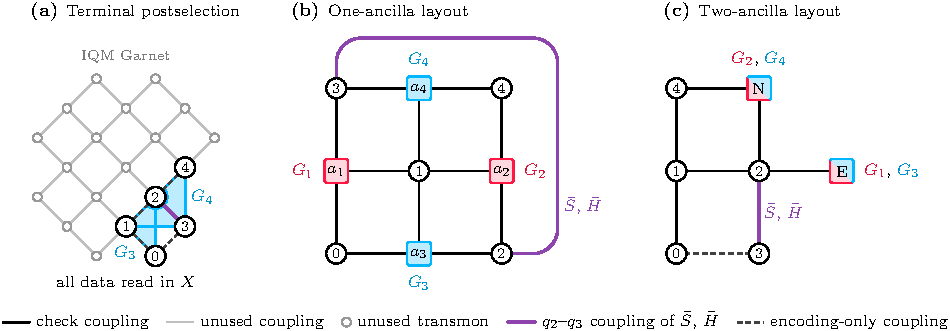
\includegraphics{figures/layouts-three.pdf}% drawn at final size
  \caption{Qutrits and couplings of the $[[5,1,2]]_3$ code in terminal postselection (a) and in the one-ancilla (b) and two-ancilla (c) layouts, with each coupling marked by its use in the stabilizer measurements, the logical gates or the encoding circuit. Circles with an index are data qutrits, small circles are unused transmons, and squares are ancillas. Red marks the $Z$-type stabilizers $G_1$, $G_2$ and blue the $X$-type $G_3$, $G_4$ (Eqs.~\eqref{eq:s1} and~\eqref{eq:s4}), and the label beside an ancilla names the stabilizers it measures in each check round. Dashed couplings are used only by the encoding circuit.
(a)~Terminal postselection on IQM's Garnet QPU, whose 20 transmons sit on a square lattice with 30 couplings between nearest neighbors~\cite{IQM240812433}. Drawn in the orientation of IQM's device map, with QB1 at the bottom, the transmons QB1, QB4, QB5, QB2 and QB6 hold $q_0, \dots, q_4$, respectively. The dashed couplings are the four that its encoding circuit uses (\autoref{fig:encoding_circuit}(a)). No ancillas are used, and the final $X$-basis readout of all data qutrits gives $G_3$ and $G_4$ (shaded; their blue outlines are not couplings, and that of $G_4$ bends around $q_2$).
(b)~One-ancilla layout on the conventional surface-code grid, with $q_1$ at the center. Ancilla $a_j$ neighbors the three data qutrits of $G_j$, and the two-qutrit gates of $\bar H$ and $\bar S$ (Eqs.~\eqref{eq:logical_H} and~\eqref{eq:logical_HS}) need a long-range coupling between $q_2$ and $q_3$. The encoding circuit of this layout (\autoref{fig:encoding_circuit}(b)) uses only check couplings, so this panel has no dashed coupling.
(c)~Two-ancilla layout: the ancillas N and E and eight couplings, all between nearest neighbors of a square lattice. N measures $G_2$ and then $G_4$, and E measures $G_1$ and then $G_3$, so each of their squares carries both colors. Neither ancilla is next to all three data qutrits of these stabilizers, so the extraction circuits (\autoref{fig:extraction_circuits}(e)--(h)) also apply SUM gates and their inverses between data qutrits, on $q_0$--$q_1$, $q_1$--$q_2$, $q_1$--$q_4$ and $q_2$--$q_3$, the coupling that also carries the two-qutrit gates of $\bar H$ and $\bar S$. The encoding circuit of this layout (\autoref{fig:encoding_circuit}(c)) uses the dashed coupling $q_0$--$q_3$ and three solid ones.}
  \label{fig:ancilla_layouts}
\end{figure*}


\begin{table}[tp]% single-column
  \centering
  \begin{tabular}{lccccc}
    \hline\hline
     & & & two-qutrit & gate & \\
     & qutrits & couplings & gates & moments & readouts \\
    \hline
    terminal & 5 & 5 & -- & -- & -- \\
    one-ancilla & 9 & 13 & 12 & 5 & 4 \\
    two-ancilla & 7 & 8 & 24 & 19 & 4 \\
    \hline\hline
  \end{tabular}
  \caption{Resources of terminal postselection and of the one-ancilla and two-ancilla layouts of \autoref{fig:ancilla_layouts}: the qutrits, the couplings used by any circuit (encoding, logical gates, check rounds), and the two-qutrit gates, gate moments and ancilla readouts of one check round. A gate moment is a set of gates on disjoint qutrits that run in parallel; a check round also has one reset moment and one readout moment in the one-ancilla layout, and one reset and two readout moments in the two-ancilla layout.}
  \label{tab:layouts}
\end{table}

\subsection{Terminal Postselection on Five Transmons}
\label{sub:layout_terminal}

\autoref{fig:ancilla_layouts}(a) places terminal postselection on IQM's Garnet QPU~\cite{IQM240812433}: the five data qutrits occupy five transmons chosen so that the four couplings of the encoding circuit and the coupling $q_2$--$q_3$ of the logical gates, all five couplings that its circuits use (\autoref{tab:layouts}), are couplings of the chip.

\subsection{One-Ancilla Layout}
\label{sub:layout_one}

The most direct way to supply the ancillas of uniform-interval postselection gives each stabilizer its own ancilla next to its three data qutrits. On the conventional surface-code grid, one data qutrit at the center of a square and four at its corners, each ancilla can neighbor all three data qutrits of its stabilizer when $q_1$, the one qutrit in all four generators, sits at the center (\autoref{fig:ancilla_layouts}(b)). Every stabilizer then acts on the center and two adjacent corners, so the ancilla $a_j$ on the site between them measures $G_j$ with one SUM gate or its inverse per data qutrit, between $H$ and $H^{-1}$ for the $X$-type generators (\autoref{fig:extraction_circuits}(a)--(d)). The round needs no gate between data qutrits, and \autoref{tab:layouts} gives its gates and its length. Of all orders of these gates that measure the four syndromes correctly, we use one with the smallest coefficient of $p^2$ in the logical error rate per round when check rounds run back to back and every round is postselected under both noise models of \autoref{sub:noise_models}, and the round is safe against single faults (\appref{app:rounds-one-ancilla}). In this layout, however, $q_2$ and $q_3$ sit at opposite corners, so the two-qutrit gates of $\bar H$ and $\bar S$ need a long-range coupling.

One may ask whether a square lattice, the connectivity of Garnet, can give each stabilizer an ancilla next to its three data qutrits and still couple $q_2$ and $q_3$. It cannot. A square lattice is bipartite, so all neighbors of a site belong to the same sublattice. An ancilla next to the data qutrits of $G_3$ puts $q_0$, $q_1$ and $q_2$ on one sublattice, and an ancilla next to those of $G_1$ puts $q_0$, $q_1$ and $q_3$ on one sublattice. Then $q_2$ and $q_3$ share a sublattice, and no coupling of the lattice joins them. The same argument with $G_2$ and $G_4$ puts $q_2$ and $q_3$ on one sublattice again. On a square lattice at least one of $G_1$ and $G_3$, and at least one of $G_2$ and $G_4$, must therefore be measured by an ancilla that does not touch all of its data qutrits, and the missing values must reach that ancilla through other gates.

\subsection{Two-Ancilla Layout}
\label{sub:layout_two}

The two-ancilla layout measures all four stabilizers in this way, with two ancillas (\autoref{fig:ancilla_layouts}(c)). The ancillas are named N and E after their positions in \autoref{fig:ancilla_layouts}(c); in each check round N measures $G_2$ and then $G_4$, and E measures $G_1$ and then $G_3$. The key idea is that a gate between two data qutrits, a data gate, can move a value from a qutrit that the ancilla does not touch onto one that it does, and can be undone afterwards. Let $z_j$ be the computational-basis value of $q_j$. To measure $G_2 = Z_1 Z_2 Z_4^{-1}$, for example, N first adds $z_2$, the value of its neighbor $q_2$. A data gate then sets $q_4$ to $z_4 - z_1$, N subtracts this value, and the data gate is undone, so that N holds $z_1 + z_2 - z_4$, the syndrome of $G_2$ (\autoref{fig:extraction_circuits}(e)). The $X$-type generators are collected in the same way between $H$ and $H^{-1}$ (\autoref{fig:extraction_circuits}(g), (h)). N and E are reset at the start of the round and read out after each of their two measurements, without a reset in between, so the second readout of each is its first readout plus the second syndrome, modulo three.

This design has a price: 16 of the 24 two-qutrit gates of the round are data gates, the round has almost four times as many gate moments as the one-ancilla round (\autoref{tab:layouts}), and a fault on a data gate can reach two data qutrits. The gates are nevertheless ordered so that the round is safe against single faults in the sense of the opening of this section (\appref{app:rounds-relay}). In return for the longer round, the two-ancilla layout fits on the square lattice of Garnet, in 48 ways of mapping its seven qutrits onto transmons such that all eight of its couplings are couplings of the chip.


\section{Circuit-Level Noise Simulations}
\label{sec:results}

% INTERIM (restructure step 1, 2026-11-19): the old Secs. 2.5, 2.7, 2.8 and 3 under one head, unchanged, until Secs. V and VI are rewritten on the new runs (two-ancilla square layout, five-moment one-ancilla round). Numbers and sentences here still describe the seven-moment round and the conventional-site two-ancilla layout.
\subsection{Noise Models}
\label{sub:noise_models}

% Sec. 2.5 (track hw). The channel formulas with their mixing forms, the scheduling rules, the two rules without effect, the three deviations from the reference models (with their TODO(authors)) and the derivation of the fault budgets are in Appendix B ("appendix - check rounds and noise.tex").
To model circuit-level noise we use qutrit forms of two models of Gidney, Newman, Fowler and Broughton~\cite{GidneyHoneycomb2021}, the superconducting-inspired model (SI1000) and the standard depolarizing model (SD6). Both attach a Pauli channel to every operation and to every idle qutrit, with a probability that is a fixed multiple of a single parameter $p$ (\autoref{tab:circuit-noise}). Three channels occur. The one-qutrit depolarizing channel DEP1 applies one of the eight non-identity Paulis $X^a Z^b$, chosen uniformly. The two-qutrit depolarizing channel DEP2 applies one of the $80$ non-identity two-qutrit Paulis, chosen uniformly. A flip applies $X$ or $X^2$, chosen uniformly, and so shifts the state that a reset prepares or the outcome of the computational-basis measurement that follows it. The parameter $p$ is the probability of DEP2, that is, the probability that a two-qutrit gate is followed by a non-identity Pauli. SI1000 makes one-qutrit gates and idling during gates ten times less noisy than two-qutrit gates, and it makes resets, measurements and idling during them two to five times noisier. SD6 gives every channel the probability $p$.

\begin{table*}[tp]
  \centering
  \begin{tabular}{l|c|c|c}
    \hline
    Circuit location & Channel & SI1000 & SD6 \\
    \hline
    After each one-qutrit gate & DEP1 & $p/10$ & $p$ \\
    After each two-qutrit gate & DEP2 & $p$ & $p$ \\
    After each reset & flip & $2p$ & $p$ \\
    Before each measurement & flip & $5p$ & $p$ \\
    Idle qutrit in a gate moment & DEP1 & $p/10$ & $p$ \\
    Idle qutrit in a reset or measurement moment & DEP1 & $2p$ & $p$ \\
    \hline
  \end{tabular}
  \caption{Qutrit SI1000 and SD6 noise models. Each entry is the probability of the channel in the second column as a multiple of $p$, the probability that a two-qutrit gate is followed by a non-identity Pauli. DEP1 and DEP2 are the one- and two-qutrit depolarizing channels, and a flip shifts the state after a reset or the outcome of a measurement. Two further rules of the models have no effect in our circuits (\appref{app:rounds}).}
  \label{tab:circuit-noise}
\end{table*}

We place the channels moment by moment, at the locations of \autoref{tab:circuit-noise}. Each logical Clifford and each check round is scheduled on its own. Gates run as early as their qutrits allow, resets and readouts occupy moments of their own, and all readouts of a round share its last moment. A qutrit that a moment leaves untouched is idle in that moment. SUM, CZ, their inverses and SWAP each count as one two-qutrit gate, which is one of three points in which these models deviate from those of~\cite{GidneyHoneycomb2021} (\appref{app:rounds}).

Two steps are noiseless in every simulation of an encoded circuit, the encoding and the final $X$-basis readout of the data qutrits. They are the state-preparation and measurement steps, whose errors in standard randomized benchmarking change the amplitude of the decay and not its rate~\cite{Magesan2011PRL,Magesan2012PRA}. Noise thus acts on the logical Cliffords, on the mirror inverse and on the check rounds.

% The four round values keep the 4p of the post-measurement DEP1 (critic round 1, B M-1 and V M1, variant (a): numbers unchanged, CONTRACT Amendment A2); without it they would be 63.9p, 72.3p, 69p and 99p. For the lead: jpw-review/handoff/hw-M2.md.
% Fault budgets: jpw-review/hw/checks/check_fault_budgets.py (.out), from the generator of the conventional-sites worktree; the round values also in paper-rework/scratch/writer-conv/budget.py (budget.out). Logical Clifford: mean over the 216 catalog words, data wires only, 5.73p (SI1000) and 28.78p (SD6).
We measure the noise of a check round or of a logical Clifford by its expected number of faults, the sum of the probabilities of its channels (\appref{app:rounds}). Under SI1000 a check round has $67.9p$ in the one-ancilla layout and $76.3p$ in the two-ancilla layout, and under SD6 it has $73p$ and $103p$. Each of these values includes $4p$ from the DEP1 that one of the two rules without effect places after the four ancilla readouts. A logical Clifford, averaged over the group, puts $5.7p$ on the data qutrits under SI1000 and $29p$ under SD6. Its idle channels on the ancillas are not counted, because the next reset erases their effect.

\subsection{Simulations}
\label{sub:sim_framework}

% Sec. 2.7 (track hw). Circuit generation, detector declarations and the comparison of the two sampling backends are in Appendix F ("sdim dem appendix.tex"). The run inventory of the former results Sec. 4.1 and of the former qubit subsection is tab:runs.
We simulate every circuit with \texttt{sdim}~\cite{sdim}, version 1.4.0, a stabilizer simulator for qudits of prime dimension. To make $10^6$ or more shots per sequence and depth affordable, we sample each circuit through a detector error model (DEM), a structure introduced for qubit circuits by Stim~\cite{Gidney2021Stim}. A detector is a combination of measurement outcomes that takes a fixed value in the absence of noise. Our detectors are the ancilla readouts of the check rounds and, for terminal postselection, the two $X$-type stabilizer values. The DEM lists, for every noise channel of a circuit, its probability and the shifts it causes in the detectors and in the logical outcome. Because all our channels are Pauli channels in Clifford circuits, sampling the DEM reproduces the joint distribution of detectors and logical outcome without approximation. After the model is built, the work per shot is proportional to the expected number of faults in the circuit, and no stabilizer computation is repeated (\appref{sec:sdim-dem}).

% Run inventory checked against the run folders by jpw-review/hw/checks/check_runs_table.py (.out): code_name.txt, noise_model.txt, num_cliffs.txt, shots.txt, depths.txt, probs.txt and check_unif.txt of the 16 runs; RB shots: NORMAL_RB_SHOTS in src/lrb/lrb_simulation.py.
\begin{table*}[tp]
  \centering
  \small
  \begin{tabular}{l|l|p{6.0cm}|p{2.7cm}|c}
    \hline
    Runs & Code & Values of $p$ & Depths $m$ & Shots \\
    \hline
    Production & qutrit, qubit & $0$; $(1, 2, 5)\times10^{-4}$; $(1, 2, 5, 7.5)\times10^{-3}$; $(1, 1.25, 1.5, 2, 3, 4, 5)\times10^{-2}$ & 0, 2, 4, 6, 10, 14, 18, 20, 22 & $10^6$ \\
    High-$p$ extension & qutrit & SI1000: $0.015$ to $0.035$ in steps of $0.0025$; $0.04$; $0.045$; $0.05$. SD6: $0.025$ to $0.06$ in steps of $0.005$ & 0, 1, 2, 3, 4, 6 & $2\times10^7$ \\
    Refinement & qubit & SI1000: $0.002$ to $0.013$ in steps of $0.0005$. SD6: $0.006$ to $0.026$ in steps of $0.001$, and in the two-ancilla layout also $0.003$ to $0.0055$ in steps of $0.0005$ & as production & $10^6$ \\
    \hline
  \end{tabular}
  \caption{Simulation runs. $p$ is the two-qutrit gate error probability, $m$ the depth and $k$ the postselection interval. Each row stands for one run per layout and noise model, four runs for each code. Shots are per sequence and depth, for the LRB-D circuits and for the circuits of terminal postselection; every baseline uses $10^4$ shots per sequence and depth. Each run draws 30 random sequences for LRB-D and 30 independent ones for its baseline. The production and refinement runs evaluate the intervals $k = 1$ to $22$, and the extension runs $k = 1$ to $6$.}
  \label{tab:runs}
\end{table*}

The simulations consist of production runs, which cover the whole range of $p$, and of additional runs near the pseudo-thresholds (\autoref{tab:runs}). Each run fixes a layout and a noise model. Its random sequences of logical Cliffords are as long as its largest depth, the circuit of depth $m$ uses the first $m$ Cliffords of a sequence, and the same sequences serve every value of $p$ and terminal postselection. Near the pseudo-thresholds the production runs reject almost every shot at the larger depths (\autoref{sub:interval_results}), so one high-$p$ extension run per layout and noise model samples twenty times more shots at depths $m \le 6$, with new sequences. Its fits, for LRB-D and for the baseline, replace the production fits at $p \ge p_{\mathrm{split}}$, with $p_{\mathrm{split}} = 0.015$ under SI1000 and $0.025$ under SD6, and for $k \ge 2$ its LRB-D fits use only the even depths (\appref{app:campaign} gives this rule and its reason). \autoref{sub:qubit_code} describes the runs of the qubit comparison.

\subsection{Qubit Code}
\label{sub:qubit_code}

% Sec. 2.8 (track hw). Former Sec. 3.5 (method.tex, lines 8-27 of the 438f6f16 mirror). The 24 Clifford words are in Appendix G, the qubit forms of the channels in Appendix B, and the search rule, the refinement grids and the overlap of production and refinement fits left for Appendix C (jpw-review/handoff/hw-moved-out.tex).
% Qubit code and catalog: FoldedQubitDetectionCode and QubitCliffordLibrary (worktree qubit-lrbd-sdim140, src/lrb/code_definitions.py), FoldedQubitConventionalSitesDetectionCode (worktree conventional-sites); checks in tests/test_folded_qubit_code.py and tests/test_conventional_sites_code.py of those worktrees.
% Qubit noise channels: sdim 1.4.0 (N1 'd' uniform over the q^2 - 1 non-identity Paulis, N1 'f' over the q - 1 nonzero shifts, N2 uniform over the q^4 - 1 non-identity Paulis) and CIRCUIT_LEVEL_NOISE_RATES in src/lrb/circuit_generator.py, identical in the qubit-lrbd-sdim140 and conventional-sites worktrees.
To separate the role of the local dimension, we repeat the simulations for the qubit $[[5,1,2]]$ code, with $q = 2$ in place of $q = 3$. Its stabilizers and logical Paulis are those of Eqs.~\eqref{eq:s1}--\eqref{eq:logicalPauli} with every exponent taken modulo two, so that $G_1 = Z_0 Z_1 Z_3$, $G_2 = Z_1 Z_2 Z_4$, $G_3 = X_0 X_1 X_2$ and $G_4 = X_1 X_3 X_4$. The gates $\bar H$ and $\bar S$ keep the form of Eqs.~\eqref{eq:logical_H} and~\eqref{eq:logical_HS}, with $H^{-1} = H$ and the qubit phase gate $S = \mathrm{diag}(1, i)$, CNOT takes the place of SUM, and the logical Cliffords are drawn from the $24$-element single-qubit Clifford group, whose words have $2.54$ primitive gates on average (\appref{sec:clifford-gen}). The noise models keep the multiples of $p$ of \autoref{tab:circuit-noise}. DEP1 applies $X$, $Z$ or $XZ$ and DEP2 one of the $15$ non-identity two-qubit Paulis, each chosen uniformly, and a flip applies $X$. With $\omega = -1$ the estimate of Eq.~\eqref{eq:estimator} becomes $\langle \bar{X} \rangle_s = P_0 - P_1$, and the error rate of Eq.~\eqref{eq:error_rate} becomes $r = (1 - f)/2$. The check rounds keep their expected numbers of faults, and a logical Clifford, whose words are shorter, puts $2.8p$ on the data qubits under SI1000 and $14.5p$ under SD6. The layouts, check rounds, postselection, mirror inverse, baseline and fits are those of the qutrit code.

Only the treatment of the region near the pseudo-thresholds differs, in two points. The search for the crossing drops two conditions of the qutrit search, a tolerance and an error floor, which are comparable to the qubit error rates at the crossings under SI1000 (\appref{app:campaign}). The qubit pseudo-thresholds also lie below the range of the high-$p$ extension, so refinement runs on a finer grid of $p$ take its place (\autoref{tab:runs}).

% Results under circuit-level SI1000 and SD6 noise (sdim 1.4.0 runs, 2026-10), Secs. 3.1 to 3.5 (track sim).
% Rewritten 2026-11-13 with the journal-paper-writing skill (PLAN Sec. 2; CONTRACT Secs. 3 to 5 and 9).
% Every number is checked against the data by paper-rework/jpw-review/sim/check_numbers.py (prose numbers:
% checks_prose.py, ids in the comments below; table bodies between "BEGIN GEN" and "END GEN" are generated
% by "check_numbers.py --write" and must not be edited by hand).
% Outline and sentence tables: paper-rework/jpw-review/sim/results-outline.md, results-sentence-tables.md.

% Scope sentence of the section (facts that the Methods leave to the Results, hand-off M1, Sec. 2).
Unless stated otherwise, the results are for the one-ancilla layout and come from the production runs; the pseudo-thresholds also use the high-$p$ extension runs (\autoref{tab:runs}). We write $r_{\mathrm{LRB}}$ and $r_{\mathrm{RB}}$ for the fitted error rates per unit of depth of LRB-D and of the baseline. We analyze the intervals $k = 1$ to $4$; for larger intervals the accepted decay departs further from a single exponential (\autoref{tab:chi_largek}, for $p = 5\times10^{-3}$).

\subsection{Terminal Postselection}
\label{sub:terminal_results}

% checks T-def-*, T-fac-*, T-p-double, T-sd6-fac (facts/raw_per_depth.csv, schedule const-0)
Under terminal postselection the accepted logical signal does not decay as a single exponential (\autoref{fig:const0_si1000_1anc}). The traces stay flat at small depth and then bend down: the deficit $1 - \langle \bar{X} \rangle$, while it is small, grows about quadratically in the depth and in $p$. Under SI1000 at $p = 10^{-3}$ it grows from $1.7\times10^{-5}$ at $m = 2$ to $2.0\times10^{-3}$ at $m = 22$, by a factor of 119 where a quadratic law gives 121, while the deficit $1 - \langle Z \rangle$ of the baseline grows by a factor of 10, where a linear law gives 11. At $m = 10$, doubling $p$ from $5\times10^{-4}$ to $10^{-3}$ multiplies the deficit by 4.0. Under SD6 the deficit grows by a factor of 28 from $m = 2$ to $10$ at $p = 10^{-3}$, where a quadratic law gives 25 (\autoref{fig:const0_sd6_1anc}). These circuits are noiseless at $m = 0$, where $\langle \bar{X} \rangle = 1$, so a single exponential would give a deficit that is linear in $m$ at small depth. We therefore extract no error rate from terminal postselection.

\begin{figure*}[tp]
  \centering
  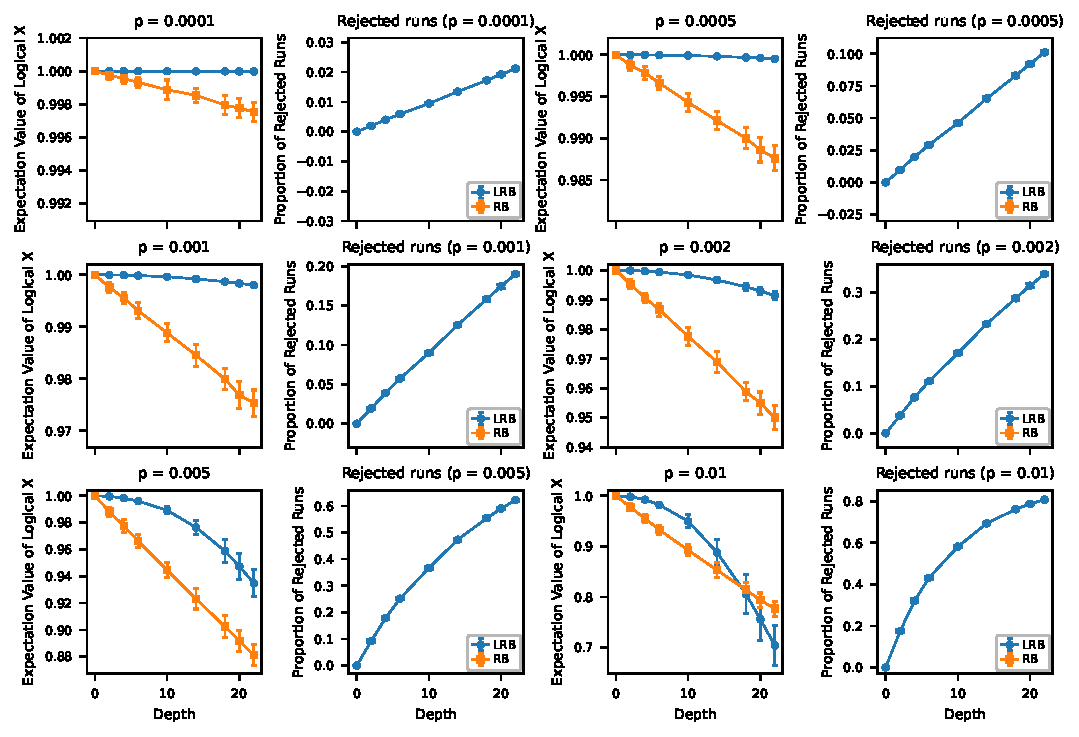
\includegraphics[width=0.95\textwidth]{figures/sdim140/si1000-1anc-const-0-nofit.pdf}
  \caption{Terminal postselection under SI1000, from the run of the one-ancilla layout, at the two-qutrit gate error probabilities $p = 10^{-4}$, $5\times10^{-4}$, $10^{-3}$, $2\times10^{-3}$, $5\times10^{-3}$ and $10^{-2}$. In each pair of panels, the left panel shows the accepted logical signal $\langle \bar{X} \rangle$ of LRB-D (blue) and the physical signal $\langle Z \rangle$ of physical RB at the same $p$ (orange) versus the depth $m$, and the right panel shows the fraction of rejected LRB-D shots; the baseline rejects none. In the figure, ``LRB'' stands for LRB-D, ``Rejected Runs'' for rejected shots, and the axis label ``Expectation Value of Logical X'' marks the signal of both curves. Error bars are standard deviations over the 30 sequences for the signals and standard errors over the sequences for the rejected fraction. The legend in each right panel labels the curves of the left panel. No fits are drawn.}
  \label{fig:const0_si1000_1anc}
\end{figure*}

% checks T-budget-*, T-model-* (raw_per_depth.csv, schedule const-0; fault counts: jpw-review/hw/checks/check_fault_budgets.out)
The quadratic growth of the deficit is that of pairs of faults. Growth as $p^2$ means that, to leading order, an accepted shot with a wrong logical outcome carries two faults, and the number of pairs of fault locations grows as $m^2$. A single fault cannot produce such a shot: the logical Cliffords keep it on one qutrit or on the pair $q_2$, $q_3$, and there it shifts the logical outcome only through a $Z$ component on $q_0$ or $q_3$, which also shifts the value of $G_3$ or $G_4$. A logical Clifford puts five times as many expected faults on the data qutrits under SD6 as under SI1000 (\autoref{sub:noise_models}), so pairs of faults predict a deficit about 25 times larger, if a pair escapes equally often under both models. At $p = 10^{-3}$ the deficit under SD6 is 32 times larger at $m = 22$, where it has reached $6.3\times10^{-2}$ and higher orders enter, and 23 to 25 times larger at the depths $m \le 6$.

% checks T-rej-*, T-sat, T-sig-sat (raw_per_depth.csv); grid points where the signal falls below the baseline: generated table const0, checks T-below-*
At large depth and $p$ terminal postselection brings no gain: it rejects most shots, and the accepted logical signal falls below the physical signal. Under SI1000 at $p = 5\times10^{-3}$ the rejected fraction is 9.2\% at $m = 2$, 37\% at $m = 10$ and 62\% at $m = 22$. The rejected fraction saturates at $8/9$, the value for uniformly random outcomes of the two $X$-type stabilizers, of whose nine joint values one is accepted; under SD6 it is $0.8889$ at $p = 10^{-2}$ and $m = 22$ (\autoref{fig:const0_sd6_1anc}). Because the deficit of LRB-D grows faster with $p$ than that of the baseline, $\langle \bar{X} \rangle$ falls below $\langle Z \rangle$ as $p$ grows, at $m = 22$ between $p = 7.5\times10^{-3}$ and $10^{-2}$ under SI1000 and between $2\times10^{-3}$ and $5\times10^{-3}$ under SD6 (\autoref{tab:const0}, which also gives $m = 10$).

% checks T-2anc-* (raw_per_depth.csv, configs conv-*); grid points: generated table const0
The run of the two-ancilla layout, whose circuits for terminal postselection are built in the same way from 30 newly drawn sequences (\autoref{sub:sim_framework}), reproduces the traces of \autoref{fig:const0_si1000_1anc} and \autoref{fig:const0_sd6_1anc} for $p$ from $10^{-3}$ to $10^{-2}$: no deficit differs between the two runs by more than two standard errors over the sequences. At $m = 10$ and $22$, its deficits agree with those of the one-ancilla run within 3\% under SI1000 and 6\% under SD6, and its rejected fractions within $0.6$ percentage points. At $m \le 6$, where the deficits are small, they differ by up to 16\%, and the deficit under SD6 at $p = 10^{-3}$ is 27 to 29 times that under SI1000. At $m = 10$ and $22$ the accepted logical signal of this run first falls below $\langle Z \rangle$ at the same grid points as in the one-ancilla run (\autoref{tab:const0}, \autoref{fig:const0_si1000_2anc}, \autoref{fig:const0_sd6_2anc}).

\subsection{Postselection on Every Check Round}
\label{sub:interval_results}

% checks K1-ratio-*, K1-exp-* (facts/fits_all_k.csv, k = 1); table body: generated table k1
With every check round postselected ($k = 1$), the fitted logical error rate per unit of depth at $p = 10^{-3}$ is smaller than that of the baseline by a factor of $92(9)$ under SI1000 and $96(2)$ under SD6, where the parentheses give the standard deviation of the parametric bootstrap (\autoref{tab:k1_error_rates}). The advantage shrinks as $p$ grows, to factors of 2.1 and 4.3 at $p = 2\times10^{-2}$, because the two error rates scale differently. Between $p = 5\times10^{-4}$ and $2\times10^{-3}$, $r_{\mathrm{LRB}}$ grows as $p^{2.0}$ under SI1000 and as $p^{1.9}$ under SD6, with uncertainties of $0.2$ and $0.03$ in the exponents, and $r_{\mathrm{RB}}$ as $p^{1.0}$ under both (\autoref{fig:four_configs} in \autoref{sub:layout_comparison} shows both rates against $p$). From $2\times10^{-3}$ to $5\times10^{-3}$ the exponents are $2.1$ and $1.6$. From $p = 5\times10^{-3}$ to $2\times10^{-2}$, $r_{\mathrm{LRB}}$ grows faster than $p^2$ under both models: as $p^{2.4}$ and $p^{2.6}$ under SI1000 and as $p^{2.1}$ and $p^{2.4}$ under SD6 in the two steps of the grid. As under terminal postselection, a single fault in a logical Clifford stays on one qutrit or on the pair $q_2$, $q_3$; there the next check round detects it. Since a single fault in a check round never leads to a logical error that this round and the next both miss (\autoref{sub:ancilla_layouts}), the nearly quadratic growth at small $p$ is again that of pairs of faults.

\begin{table*}[tp]
  \centering
  \small
  \begin{tabular}{c|ccc|ccc}
    \hline
    & \multicolumn{3}{c|}{SI1000} & \multicolumn{3}{c}{SD6} \\
    $p$ & $r_{\mathrm{LRB}}$ & $r_{\mathrm{RB}}$ & $r_{\mathrm{RB}}/r_{\mathrm{LRB}}$ & $r_{\mathrm{LRB}}$ & $r_{\mathrm{RB}}$ & $r_{\mathrm{RB}}/r_{\mathrm{LRB}}$ \\
    \hline
    % BEGIN GEN k1
    $10^{-3}$ & $(8.3 \pm 0.8)\times10^{-6}$ & $7.6\times10^{-4}$ & $92 \pm 9$ & $(8.26 \pm 0.18)\times10^{-5}$ & $8.0\times10^{-3}$ & $96 \pm 2$ \\
    $5\times10^{-3}$ & $(2.27 \pm 0.12)\times10^{-4}$ & $3.8\times10^{-3}$ & $16.8 \pm 0.9$ & $(1.38 \pm 0.04)\times10^{-3}$ & $3.9\times10^{-2}$ & $28.1 \pm 0.8$ \\
    $10^{-2}$ & $(1.16 \pm 0.04)\times10^{-3}$ & $7.6\times10^{-3}$ & $6.6 \pm 0.2$ & $(6.05 \pm 0.20)\times10^{-3}$ & $7.6\times10^{-2}$ & $12.5 \pm 0.4$ \\
    $2\times10^{-2}$ & $(7.15 \pm 0.24)\times10^{-3}$ & $1.5\times10^{-2}$ & $2.10 \pm 0.07$ & $(3.29 \pm 0.21)\times10^{-2}$ & $1.4\times10^{-1}$ & $4.3 \pm 0.3$ \\
    % END GEN k1
    \hline
  \end{tabular}
  \caption{Fitted error rates per unit of depth in the one-ancilla layout, from the production runs, at four values of the two-qutrit gate error probability $p$: $r_{\mathrm{LRB}}$ for LRB-D with the postselection interval $k = 1$, $r_{\mathrm{RB}}$ for the baseline, physical RB under the same noise model at the same $p$, and their ratio. The uncertainties of $r_{\mathrm{LRB}}$ and of the ratio are standard deviations of the parametric bootstrap, which do not include the choice of sequences; that of $r_{\mathrm{RB}}$ is below 1\% of its value and is not shown. \autoref{tab:k1_depths} gives the number of depths in each fit.}
  \label{tab:k1_error_rates}
\end{table*}

% checks K1-rej-* (raw_per_depth.csv, schedule unif-1)
These error rates describe a fraction of the shots that shrinks with depth. Under SI1000 at $p = 5\times10^{-3}$ the postselection rejects 22\% of the shots at $m = 0$, 63\% at $m = 2$, 98.1\% at $m = 10$ and 99.98\% at $m = 22$, where about 200 of $10^6$ shots per sequence are accepted. The rejected fraction is smaller at smaller $p$, 55\% at $m = 10$ for $p = 10^{-3}$, and at $m = 10$ it is larger under SD6, 99.8\% for $p = 5\times10^{-3}$ (right panels of \autoref{fig:unif1_si1000_1anc} and \autoref{fig:unif1_sd6_1anc}).

\begin{figure*}[tp]
  \centering
  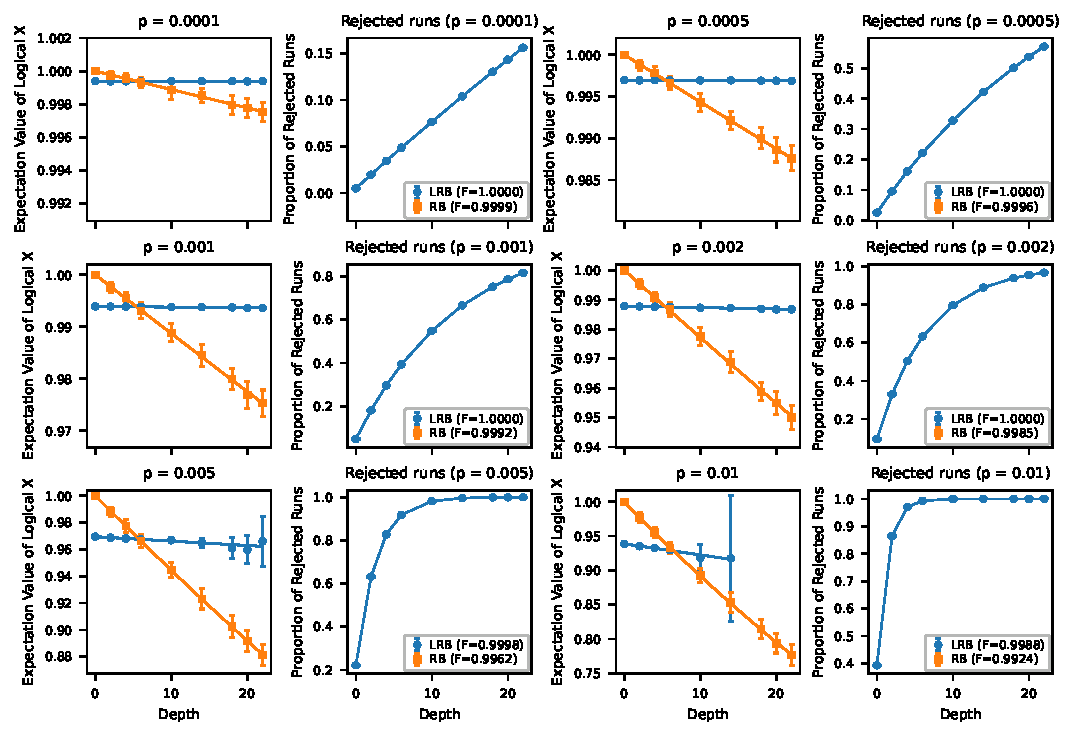
\includegraphics[width=0.95\textwidth]{figures/sdim140/si1000-1anc-unif-1-fit.pdf}
  \caption{Uniform-interval postselection with interval $k = 1$ under SI1000 in the one-ancilla layout, at the two-qutrit gate error probabilities $p = 10^{-4}$, $5\times10^{-4}$, $10^{-3}$, $2\times10^{-3}$, $5\times10^{-3}$ and $10^{-2}$. Left panels: accepted logical signal $\langle \bar{X} \rangle$ of LRB-D (blue; ``LRB'' in the legend) and physical signal $\langle Z \rangle$ of physical RB at the same $p$ (orange) versus the depth $m$, with the fits $F(m) = A f^m$ (lines); the axis label ``Expectation Value of Logical X'' marks the signal of both curves, and the legends in the right panels give the fitted average fidelity $\bar{F}$ per unit of depth as ``F''. Right panels: fraction of rejected LRB-D shots (``Rejected Runs''). Error bars are standard deviations over the 30 sequences for the signals and standard errors over the sequences for the rejected fraction. LRB-D points are missing at depths where a sequence has no accepted shot.}
  \label{fig:unif1_si1000_1anc}
\end{figure*}

% checks K1-chi-* (facts/fit_chi2.csv: lrb_chi2/(lrb_n_points - 2)), K1-slope-* (raw_per_depth.csv, 1anc-sd6)
The single exponential fitted for $r_{\mathrm{LRB}}$ describes the accepted decay approximately under SD6 and closely under SI1000 (\autoref{fig:unif1_si1000_1anc}, \autoref{fig:unif1_sd6_1anc}). Under SD6 the decay steepens with depth: at $p = 10^{-3}$ the signal drops by $6.6\times10^{-5}$ per unit of depth between $m = 0$ and $6$ and by $3.0\times10^{-4}$, 4.6 times as fast, between $m = 18$ and $22$. The steepening is consistent with the mirror inverse, in which no check round separates the Cliffords, so that pairs of faults accumulate as under terminal postselection, and with the larger expected number of faults of a logical Clifford under SD6. The SD6 values of $r_{\mathrm{LRB}}$, of the ratios of \autoref{tab:k1_error_rates} and of the exponents above are therefore effective values over the fitted depths, and their uncertainties do not include the dependence on these depths. Against the value $1/N_s = 0.03$ for residuals of the size of the standard errors (\autoref{sub:fit_model}), $\chi^2$ per degree of freedom for $10^{-3} \le p \le 10^{-2}$ is $0.5$ to $2.1$ under SD6 and $0.01$ to $0.07$ under SI1000 (\autoref{tab:k1_depths}).

% checks K1-m0-*, K1-A, K1-cross, K1-slow (raw_per_depth.csv, fits_all_k.csv); full set: generated table m0; fault count of the loss: checks K1-m0-count-* (round schedule in jpw-review/hw/checks/check_single_faults.out, rates of tab:circuit-noise)
The traces start below one, because some single faults in the final check round, which no later round follows, escape detection. At $m = 0$ the circuit applies one check round between the noiseless encoding and readout, and $\langle \bar{X} \rangle$ is $0.9695$ under SI1000 and $0.9415$ under SD6 at $p = 5\times10^{-3}$. This deficit at depth zero, which we call the loss, is about $6p$ and $12p$ (\autoref{tab:m0}). The loss comes from the faults on $q_0$ and $q_3$, the two qutrits that are read, after their last two-qutrit gate of the final check round: the channels at these locations shift the logical outcome with probability $4.05p$ under SI1000 and $7.95p$ under SD6, which lowers the signal by $6.1p$ and $11.9p$, as measured at $p = 10^{-3}$ (\autoref{tab:m0}). At $p = 5\times10^{-3}$ the loss is why the LRB-D trace of \autoref{fig:unif1_si1000_1anc}, although it decays 17 times more slowly, starts below the baseline trace and crosses it between $m = 4$ and $6$. Like every error that does not depend on the depth (\autoref{sub:fit_model}), the loss goes into the fitted amplitude, which there equals the signal at depth zero to four digits, and to leading order not into $f$.

\subsection{Pseudo-Thresholds}
\label{sub:pseudo_thresholds}

% p* and seq_boot_se: comparisons/pseudo-thresholds-current.csv (one-ancilla rows) and pseudo-thresholds-conv-sites-current.csv; checks P-*; table body: generated table pstar
In the one-ancilla layout with $k = 1$, the logical error rate stays below that of the baseline up to $p^\star(1) = 0.0292(6)$ under SI1000 and up to $p^\star(1) = 0.0399(15)$ under SD6 (\autoref{tab:pseudo_thresholds}; \autoref{fig:threshold_grid_si1000_1anc}, \autoref{fig:threshold_grid_sd6_1anc}). The pseudo-threshold falls as fewer check rounds enter the postselection, by a factor of 2.2 from $k = 1$ to $4$ under SI1000 and by a factor of 2.6 under SD6.

\begin{table*}[tp]
  \centering
  \small
  \setlength{\tabcolsep}{4pt}
  \begin{tabular}{c|cccc|cccc}
    \hline
    & \multicolumn{4}{c|}{SI1000} & \multicolumn{4}{c}{SD6} \\
    $k$ & one-ancilla & two-ancilla & gap (\%) & in s.e. & one-ancilla & two-ancilla & gap (\%) & in s.e. \\
    \hline
    % BEGIN GEN pstar
    1 & $0.0292 \pm 0.0006$ & $0.0266 \pm 0.0004$ & $8.8 \pm 2.3$ & 3.9 & $0.0399 \pm 0.0015$ & $0.0283 \pm 0.0007$ & $29.0 \pm 3.1$ & 9.2 \\
    2 & $0.0239 \pm 0.0005$ & $0.0209 \pm 0.0003$ & $12.6 \pm 2.2$ & 5.6 & $0.0269 \pm 0.0007$ & $0.0212 \pm 0.0003$ & $21.2 \pm 2.3$ & 9.1 \\
    3 & $0.0166 \pm 0.0004$ & $0.0136 \pm 0.0003$ & $17.9 \pm 2.9$ & 6.2 & $0.0181 \pm 0.0006$ & $0.0122 \pm 0.0003$ & $32.4 \pm 2.8$ & 11.6 \\
    4 & $0.0132 \pm 0.0002$ & $0.0108 \pm 0.0001$ & $17.9 \pm 1.6$ & 10.9 & $0.0155 \pm 0.0004$ & $0.0103 \pm 0.0001$ & $33.4 \pm 2.1$ & 15.8 \\
    % END GEN pstar
    \hline
  \end{tabular}
  \caption{Pseudo-thresholds $p^\star(k)$ of the $[[5,1,2]]_3$ code against the baseline, physical RB under the same noise model at the same two-qutrit gate error probability $p$, for the postselection intervals $k = 1$ to $4$ and the two layouts; the gap $1 - p^\star_{\mathrm{two}}/p^\star_{\mathrm{one}}$ between the layouts in percent; and its size in units of its standard error (s.e.), computed before rounding. Uncertainties are one standard error (68\% confidence), from a bootstrap over the random Clifford sequences. The relative standard error of the ratio $p^\star_{\mathrm{two}}/p^\star_{\mathrm{one}}$ is the two relative standard errors added in quadrature, and the standard error of the gap is that of the ratio (\appref{app:campaign-bootstrap}).}
  \label{tab:pseudo_thresholds}
\end{table*}

\begin{figure*}[tp]
  \centering
  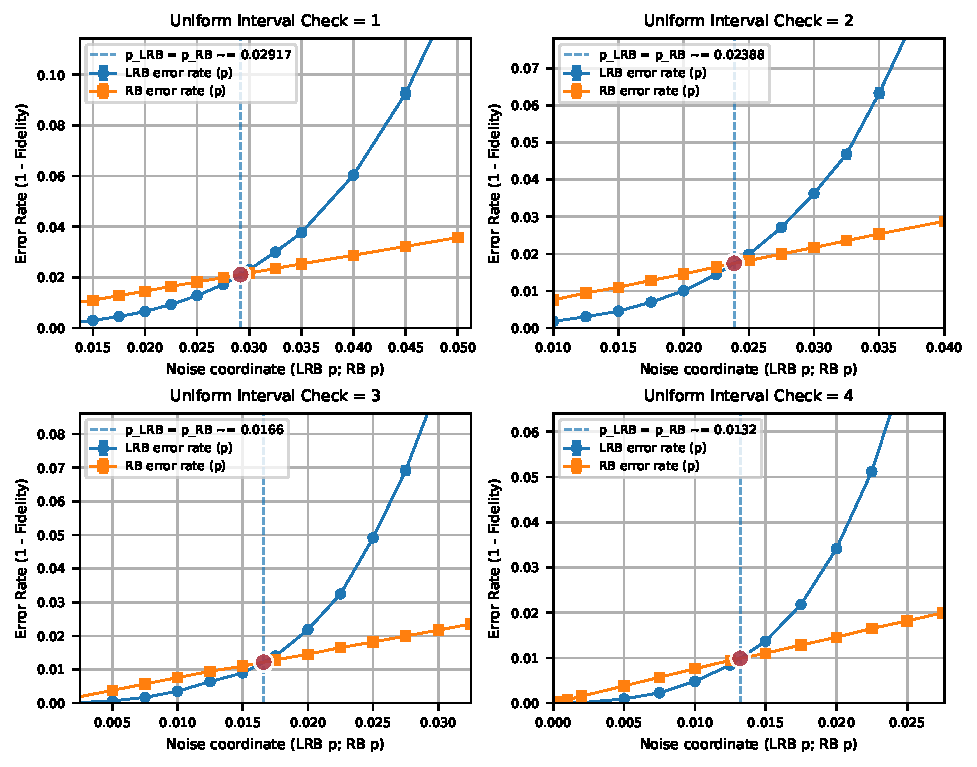
\includegraphics[width=0.75\textwidth]{figures/sdim140/si1000-1anc-threshold-grid.pdf}
  \caption{Fitted error rates per unit of depth of LRB-D (blue) and of the baseline, physical RB (orange), versus the two-qutrit gate error probability $p$ under SI1000 in the one-ancilla layout, for the intervals $k = 1$ to $4$, with central 68\% intervals of the parametric bootstrap; intervals that are not visible are smaller than the markers. Each panel shows a window around $p^\star(k)$ of the grid that merges the two runs: points at $p < 0.015$ come from the production run and points at $p \ge 0.015$ from the high-$p$ extension run, and the $k = 1$ panel shows only the latter. The panel titles give the interval $k$, the horizontal axis is $p$ for both curves, ``LRB'' and ``RB'' in the legends stand for LRB-D and the baseline, ``Error Rate (1 - Fidelity)'' is the error rate per unit of depth, and the first legend entry gives $p^\star(k)$. The vertical line and the large marker of each panel give the pseudo-threshold $p^\star(k)$ of \autoref{tab:pseudo_thresholds}.}
  \label{fig:threshold_grid_si1000_1anc}
\end{figure*}

% checks P-kdep-* (fits_all_k.csv, raw_per_depth.csv); full set: generated table kdep
Because all intervals of a production run share one set of circuits and shots (\autoref{sub:lrb_d}), a change of $k$ at fixed $p$ changes only which shots are accepted. Postselecting fewer rounds accepts more shots and raises $r_{\mathrm{LRB}}$ (\autoref{tab:kdep}, for $p = 5\times10^{-3}$ and $10^{-2}$; \autoref{fig:unif2_si1000_1anc} to \autoref{fig:unif4_sd6_1anc} show the traces). Under SI1000 at $p = 5\times10^{-3}$, the rejected fraction at $m = 10$ falls from its value at $k = 1$ (\autoref{sub:interval_results}) to 93.7\% at $k = 4$, while $r_{\mathrm{LRB}}$ rises by a factor of 4.1; under SD6 at the same $p$ the factor is 3.8. The rise is consistent with the pairs of faults of \autoref{sub:terminal_results}, which a round outside the postselection no longer separates: for $k = 2$ to $4$, $r_{\mathrm{LRB}}$ still grows as $p^{2.0}$ to $p^{2.1}$ between $p = 5\times10^{-4}$ and $2\times10^{-3}$. The fall of the pseudo-threshold with $k$ thus comes from $r_{\mathrm{LRB}}$ alone, because the baseline does not depend on $k$.

% checks P-model-* (canonical files), P-lrb-model, P-rb-model (fits_all_k.csv, p = 0.01, k = 1); full set: generated table model_ratio
In the one-ancilla layout the SD6 pseudo-thresholds exceed the SI1000 ones at every interval, by 9 to 37\%, which is 1.9 to 6.5 standard errors of their ratio (\autoref{tab:model_ratio}). At $p = 10^{-2}$ and $k = 1$, $r_{\mathrm{LRB}}$ is 5.2 times as large under SD6 as under SI1000, so the higher SD6 values do not come from a lower logical error rate (\autoref{tab:kdep} gives the other intervals). The baseline, whose gates fail with probability $p$ under SD6 and $p/10$ under SI1000 (\autoref{tab:circuit-noise}), has an error rate 10 times as large; the SD6 pseudo-thresholds are higher because the baseline grows by more than the logical error rate.

% checks P-acc-min, P-chi-* (merged tables: lrb_chi2/(lrb_n_points - 2), p = 0.015 to 0.035); brackets: generated table brackets
Two limits apply near the pseudo-thresholds. First, many of the fits that bracket them have few depths, and some have few accepted shots at their largest depth (\autoref{tab:brackets}). Eleven of the sixteen values of \autoref{tab:pseudo_thresholds}, among them all eight with $k \le 2$, rest on the depths $m \le 6$ alone, and under SD6 the fits that bracket $p^\star(1)$ and $p^\star(2)$ have three to five depths. Seven of the 32 bracketing fits, all for $k = 1$ or $4$, have fewer than ten accepted shots per sequence at their largest depth, down to $3.6$. With so few shots the modulus of the estimate is biased upward (\appref{app:campaign-fits}), which acts to lower the fitted $r_{\mathrm{LRB}}$ and to raise $p^\star$; the standard errors do not include this bias. Second, as under SD6 already for $k = 1$ (\autoref{sub:interval_results}), a single exponential is approximate near the SI1000 pseudo-thresholds for $k = 3$ and $4$; for $k \le 2$ it describes the decays closely. Under SI1000 between $p = 0.015$ and $0.035$, in both layouts, $\chi^2$ per degree of freedom is $0.1$ to $1.1$ for $k = 1$ and $2$, which is 4 to 33 times the value $1/N_s$ of \autoref{sub:fit_model}, and $1.3$ to $9.6$ for $k = 3$ and $4$, where the traces step at depths that are not multiples of $k$ (\appref{app:campaign-search}). The bracketing fits at $p < 0.015$, for $k = 4$ and for $k = 3$ in the two-ancilla layout, lie in the same range (\autoref{tab:brackets_rates}). Under SI1000, for $k = 3$ and $4$ the extension and the production fit at the same $p$, which hold different depths, differ by up to 16\% in $r_{\mathrm{LRB}}$ (\appref{app:campaign-runs}).

% checks P-step-min, P-order (sequence-bootstrap replicate files; full set: generated table fall_factors)
Within these limits, each of the sixteen entries of \autoref{tab:pseudo_thresholds} lies between two neighboring grid points at which $r_{\mathrm{LRB}}$ is below and above $r_{\mathrm{RB}}$, and for each of the sixteen the difference of the two changes sign nowhere else on its grid of $p$ (\autoref{tab:brackets}, \autoref{tab:brackets_rates}). Every step between adjacent intervals amounts to at least 6 standard errors when the bootstrap replicates are paired over the sequences that the intervals share, and the ordering $p^\star(1) > p^\star(2) > p^\star(3) > p^\star(4)$ holds in all 1000 replicates of every layout and noise model (\autoref{tab:fall_factors}).

\subsection{Two-Ancilla Layout}
\label{sub:layout_comparison}

% Layout gaps 1 - p*(two)/p*(one), relative standard errors in quadrature: generated table pstar; checks L-*
% Rejected fractions and fitted errors: raw_per_depth.csv, fits_all_k.csv (configs conv-*)
The longer check round of the two-ancilla layout lowers every pseudo-threshold, by 9 to 18\% under SI1000 and by 21 to 33\% under SD6 (\autoref{tab:pseudo_thresholds}). Each of these eight gaps between the layouts is 3.9 to 15.8 times its standard error. Because these standard errors include the choice of the baseline sequences (\autoref{sub:fit_model}), they account for the differences between the baseline error rates of the runs of the two layouts, which reach 9\% (\autoref{tab:rb_layouts}).

At equal $p$ and $k = 1$, the two-ancilla layout rejects more shots wherever shots are accepted, and its fitted $r_{\mathrm{LRB}}$ is the larger one at each of the ten grid points from $p = 5\times10^{-4}$ to $0.03$ (\autoref{fig:four_configs}; \autoref{fig:unif1_si1000_2anc} to \autoref{fig:threshold_grid_sd6_2anc}). Under SI1000 the two error rates differ by 0.8 to 4.1 standard deviations of the parametric bootstrap of their ratio over the ten grid points; $r_{\mathrm{LRB}}$ is larger by 16\% at $p = 5\times10^{-3}$ and by 12\% at $10^{-2}$ (2.0 and 2.1 standard deviations). Under SD6 it is larger by 56\% and 78\% at these two $p$ (9.1 and 8.6 standard deviations). At $p = 5\times10^{-3}$ a single round, at $m = 0$, rejects $24.8\%$ of the shots under SI1000 and $28.5\%$ under SD6, $2.7$ and $8.5$ percentage points more than in the one-ancilla layout (\autoref{tab:m0}).

\begin{figure*}[tp]
  \centering
  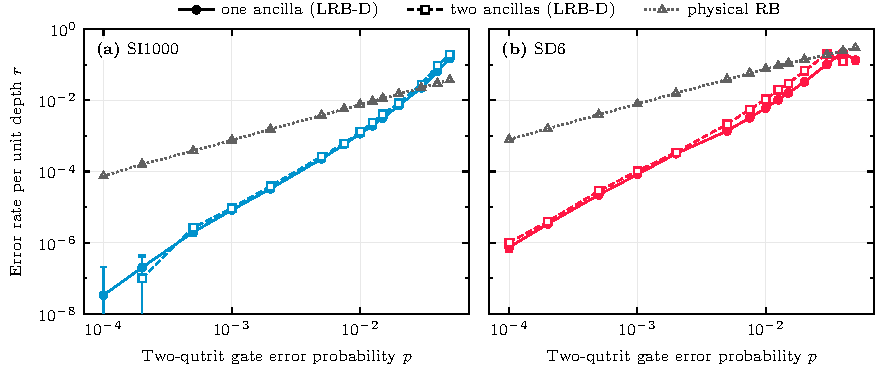
\includegraphics{figures/sdim140/lrb-vs-rb-k1.pdf}
  \caption{Fitted error rate per unit of depth for LRB-D with the postselection interval $k = 1$ versus the two-qutrit gate error probability $p$ under (a)~SI1000 and (b)~SD6, in the one-ancilla layout (filled circles, solid lines) and the two-ancilla layout (open squares, dashed lines), and for the baseline, physical RB under the same noise model, in the one-ancilla runs (open triangles, dotted lines). Error bars are central 68\% intervals of the parametric bootstrap; bars that are not visible are smaller than the markers, and intervals that reach zero run to the bottom of the axis. All points are fits to the production runs. At $p \ge 0.03$ every LRB-D fit rests on two or three depths (\autoref{tab:k1_depths}); the downturns of the SD6 curves at the largest $p$ come from such fits, and fits that return zero error are not drawn. The pseudo-thresholds of \autoref{tab:pseudo_thresholds} use the high-$p$ extension runs from $p = 0.015$ (SI1000) and $0.025$ (SD6) on, so they cannot be read off the crossings drawn here.}
  \label{fig:four_configs}
\end{figure*}

% Fault counts per round: Sec. 2.5 (67.9p, 76.3p, 73p, 103p; hw checks/check_fault_budgets.py); idle locations: scratch/writer-conv/budget.out; checks L-budget-*, L-gapdiff-*, L-rb-max
The gap is larger under SD6 at every interval, by 9 to 20 percentage points, which is 2.7 standard errors at $k = 2$ and 3.6 to 5.8 at the other intervals (\autoref{tab:model_ratio}). The fault counts go the same way: the data relay raises the expected number of faults per round by $8.4p$ under SI1000 and by $30p$ under SD6 (\autoref{sub:noise_models}), and under SD6 $22p$ of the $30p$ come from the 22 additional idle locations of the four extra gate moments, which SI1000 charges at $p/10$ (\appref{app:rounds-budget}).

% checks L-model-max, L-lrb-model, L-rb-model (fits_all_k.csv, configs conv-*, p = 0.01, k = 1)
With the larger gap under SD6, the two noise models give pseudo-thresholds within about 10\% of each other in the two-ancilla layout, at most 3.3 standard errors apart (\autoref{tab:model_ratio}). From SI1000 to SD6, $r_{\mathrm{LRB}}$ at $p = 10^{-2}$ and $k = 1$ now grows by a factor of 8.3, close to the factor of 9.5 by which the baseline of the same runs grows.

\subsection{Comparison with the Qubit Code}
\label{sub:qubit_comparison}

% Qubit p* and seq_boot_se: comparisons/pseudo-thresholds-qubit-current.csv (qubit-one-ancilla rows only) and pseudo-thresholds-qubit-conv-sites-current.csv; table body: generated table qubit; checks Q-*
For the qubit $[[5,1,2]]$ code every pseudo-threshold lies below that of the qutrit code in the same layout, under the same noise model and at the same interval (\autoref{tab:pseudo_thresholds_qubit}, \autoref{fig:pstar_qubit_qutrit}). The ratio $p^\star_{\mathrm{qubit}}/p^\star_{\mathrm{qutrit}}$ is 0.29 to 0.38 under SI1000 and 0.45 to 0.56 under SD6, and each of the sixteen ratios lies more than 15 standard errors below one. On the qutrit grids the tolerance and the error floor that the qubit search omits (\autoref{sub:qubit_code}, \appref{app:campaign-search}) change none of the sixteen values of \autoref{tab:pseudo_thresholds}, so each ratio compares two crossings located by the same search rule. Both limits of \autoref{sub:pseudo_thresholds} apply to the qubit values as well. Three of their 32 bracketing fits, all under SD6, have fewer than ten accepted shots per sequence at their largest depth; the fits that bracket $p^\star(1)$ and $p^\star(2)$ under SD6 again have three to five depths, and those under SI1000 have six or nine. $\chi^2$ per degree of freedom of the bracketing fits is $0.01$ to $0.5$ for $k \le 2$ and $0.7$ to $2.3$ for $k = 3$ and $4$ (\autoref{tab:brackets_qubit}, \autoref{tab:brackets_rates_qubit}). Within these limits, all sixteen qubit values are crossings between two neighboring points of the refinement runs.

\begin{table*}[tp]
  \centering
  \begin{tabular}{cc|cc|cc}
    \hline
    & & \multicolumn{2}{c|}{SI1000} & \multicolumn{2}{c}{SD6} \\
    layout & $k$ & $p^\star_{\mathrm{qubit}}$ & $p^\star_{\mathrm{qubit}}/p^\star_{\mathrm{qutrit}}$ & $p^\star_{\mathrm{qubit}}$ & $p^\star_{\mathrm{qubit}}/p^\star_{\mathrm{qutrit}}$ \\
    \hline
    % BEGIN GEN qubit
    one-ancilla & 1 & $0.0112 \pm 0.0002$ & $0.38 \pm 0.01$ & $0.0210 \pm 0.0008$ & $0.53 \pm 0.03$ \\
     & 2 & $0.0078 \pm 0.0002$ & $0.33 \pm 0.01$ & $0.0151 \pm 0.0005$ & $0.56 \pm 0.02$ \\
     & 3 & $0.00495 \pm 0.00009$ & $0.30 \pm 0.01$ & $0.0094 \pm 0.0003$ & $0.52 \pm 0.02$ \\
     & 4 & $0.00395 \pm 0.00008$ & $0.30 \pm 0.01$ & $0.0072 \pm 0.0002$ & $0.47 \pm 0.02$ \\
    \hline
    two-ancilla & 1 & $0.0093 \pm 0.0001$ & $0.35 \pm 0.01$ & $0.0142 \pm 0.0004$ & $0.50 \pm 0.02$ \\
     & 2 & $0.0064 \pm 0.0001$ & $0.31 \pm 0.01$ & $0.0100 \pm 0.0003$ & $0.47 \pm 0.01$ \\
     & 3 & $0.00395 \pm 0.00008$ & $0.29 \pm 0.01$ & $0.0061 \pm 0.0002$ & $0.50 \pm 0.02$ \\
     & 4 & $0.00313 \pm 0.00005$ & $0.29 \pm 0.01$ & $0.0047 \pm 0.0001$ & $0.45 \pm 0.01$ \\
    % END GEN qubit
    \hline
  \end{tabular}
  \caption{Pseudo-thresholds $p^\star(k)$ of the qubit $[[5,1,2]]$ code against single-qubit RB under the same noise model at the same two-qubit gate error probability $p$, for the postselection intervals $k = 1$ to $4$, and their ratio to the qutrit values of \autoref{tab:pseudo_thresholds} for the same layout, noise model and interval. Uncertainties are one standard error (68\% confidence), from a bootstrap over the random Clifford sequences. The relative standard error of a ratio is the two relative standard errors added in quadrature (\appref{app:campaign-bootstrap}).}
  \label{tab:pseudo_thresholds_qubit}
\end{table*}

\begin{figure*}[tp]
  \centering
  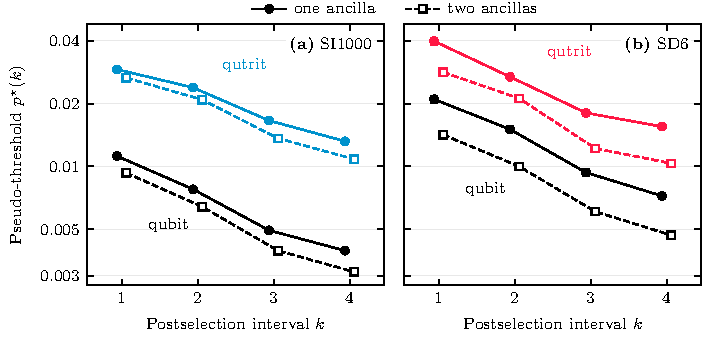
\includegraphics{figures/sdim140/pstar-qubit-vs-qutrit.pdf}
  \caption{Pseudo-threshold $p^\star(k)$ versus the postselection interval $k$ for the $[[5,1,2]]_3$ code (qutrit; blue in (a), red in (b)) and the qubit $[[5,1,2]]$ code (black) under (a)~SI1000 and (b)~SD6, in the one-ancilla layout (filled circles, solid lines) and the two-ancilla layout (open squares, dashed lines). Each $p^\star$ is the crossing of the LRB-D error rate with the error rate of physical RB of the same local dimension under the same noise model. Error bars are one standard error (68\% confidence) from the bootstrap over the random Clifford sequences; bars that are not visible are smaller than the markers. For legibility the two layouts are drawn $0.06$ to the left and right of each $k$, and the lines guide the eye.}
  \label{fig:pstar_qubit_qutrit}
\end{figure*}

% checks Q-fall-*, Q-gap-* (canonical files, replicate files); full sets: generated tables fall_factors, qubit_layout_gap
The qubit pseudo-thresholds depend on the interval and on the layout in the same directions as the qutrit ones. They fall with $k$ in all 1000 replicates of every layout and noise model, by factors of 2.8 to 3.0 from $k = 1$ to $4$. Each factor is 1.1 to 1.3 times the qutrit factor of the same layout and noise model, a difference of 7.0 and 8.6 standard errors of their ratio under SI1000 and of 2.2 and 2.9 under SD6 (\autoref{tab:fall_factors}). The two-ancilla layout lowers them by 17 to 21\% under SI1000 and by 32 to 35\% under SD6, which is 7.9 to 12.6 standard errors (\autoref{tab:qubit_layout_gap}).

% checks Q-rb-*, Q-est-* (refits of the production runs; word lengths from the RB circuits); full set: generated table rb_ratio
Of the two error rates that cross at a pseudo-threshold, the baseline error rate is smaller for the qubit code at equal $p$. In the production runs of both layouts, at every $p > 0$ of the grid, the qubit $r_{\mathrm{RB}}$ is 0.44 to 0.48 times the qutrit one under SI1000 and 0.42 to 0.49 times under SD6 (\autoref{tab:rb_ratio}; \autoref{fig:k1_qubit_qutrit} shows the one-ancilla layout; \appref{app:campaign-fits} gives the factor that converts these ratios to $1 - f$). The error added per gate and the number of gates per Clifford account for this ratio. To first order in its probability $p_1$, the DEP1 channel after a primitive gate adds $q\,p_1/(q+1)$ to the error rate, that is, $2p_1/3$ for a qubit and $3p_1/4$ for a qutrit. With the mean numbers of primitive gates per Clifford of \autoref{sub:qubit_code} and \autoref{sub:fit_model}, these give a ratio of $8/9$ times the ratio of the two means, 0.44. With the numbers drawn in the qubit and the qutrit run of each layout and noise model, the estimate stays within 0.02 of the fitted ratio of these two runs for every $p \le 10^{-2}$ (\autoref{tab:rb_ratio}; \appref{app:campaign-data} extends the estimate to larger $p$).

\begin{figure*}[tp]
  \centering
  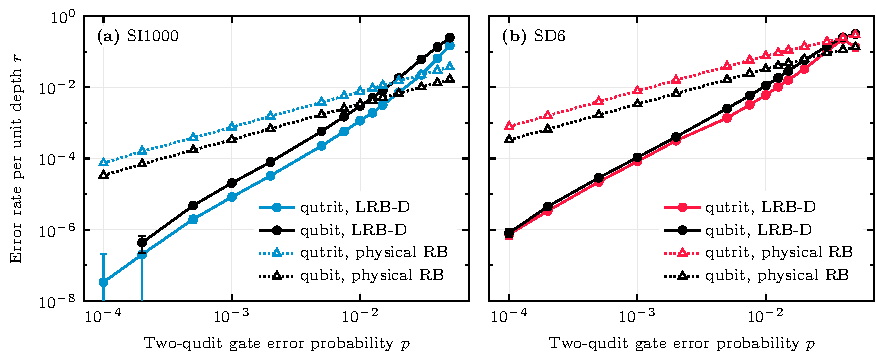
\includegraphics{figures/sdim140/lrb-vs-rb-k1-qubit-vs-qutrit.pdf}
  \caption{Fitted error rate per unit of depth versus the two-qudit gate error probability $p$ for the $[[5,1,2]]_3$ code (qutrit; blue in (a), red in (b)) and the qubit $[[5,1,2]]$ code (black) in the one-ancilla layout under (a)~SI1000 and (b)~SD6: LRB-D with the postselection interval $k = 1$ (filled markers, solid lines) and the baseline, physical RB of the same local dimension (open triangles, dotted lines). The error rate is $r = (q-1)(1-f)/q$ for local dimension $q$ and decay parameter $f$. Error bars are central 68\% intervals of the parametric bootstrap; bars that are not visible are smaller than the markers, and intervals that reach zero run to the bottom of the axis. All points are fits to the production runs. At $p \ge 0.03$ every LRB-D fit rests on two or three depths. The qubit LRB-D fit at $p = 10^{-4}$ under SI1000 returns zero error and is not drawn.}
  \label{fig:k1_qubit_qutrit}
\end{figure*}

% checks Q-lrb-*, Q-ex-*, Q-rej-*, Q-gates-* (refits of the production runs; scratch/writer-qubit/analysis.out X6); full set: generated table lrb_ratio
The logical error rate, in contrast, is larger for the qubit code. In both layouts, under both noise models and for $k = 1$ to $4$, the qubit $r_{\mathrm{LRB}}$ exceeds the qutrit one at every grid point of the production runs from $p = 10^{-3}$ up to the qutrit pseudo-threshold, by more than three standard deviations of the parametric bootstrap of their ratio. Between $p = 10^{-3}$ and $10^{-2}$ it is 2.4 to 3.0 times as large under SI1000 and 1.3 to 2.1 times under SD6 (\autoref{tab:lrb_ratio}; \autoref{fig:k1_qubit_qutrit} shows $k = 1$ in the one-ancilla layout). These error rates describe a larger fraction of the shots, since the qutrit code rejects more wherever both codes accept any: under SI1000 at $p = 5\times10^{-3}$ and $k = 1$ the qubit code rejects 60\% of the shots at $m = 2$ and 97\% at $m = 10$ (\autoref{tab:rej_qubit}; \autoref{sub:interval_results} gives the qutrit values). The mechanism behind the larger qubit logical error rate is open. With the same expected number of faults in a check round and about half as many in a logical Clifford as the qutrit code (\autoref{sub:noise_models}, \autoref{sub:qubit_code}), the qubit circuits hold fewer expected faults at equal $p$, so the number of faults does not explain it. The lower qubit pseudo-thresholds thus combine both differences: a smaller baseline error rate and a larger logical error rate each move the crossing to smaller $p$.




\FloatBarrier
% Sec. 4, Discussion and Conclusion (track sim, 2026-11-13; rewritten after critic round 1,
% jpw-review/sim/critiques/disc_critique_round1.md, adjudication in jpw-review/sim/disc_round1_adjudication.md).
% Structure (LDR): a lead that states the answer and the threads; what qualifies the answer (limits as links to
% Secs. 2.3 and 3.3 and three further points; LI4); what a pseudo-threshold compares; how the schedule and the
% layout act; consequences for an experiment (hardware appears only as an outlook, CONTRACT Sec. 6; no device is
% named); a resolution that synopsizes in words, answers the question of Sec. 1 and returns to its gap (RS8).
% No numeral of Sec. 3 is repeated (CONTRACT Sec. 5.7); the statements in words are checked against the data by
% jpw-review/sim/checks_appendix.py (ids S4-*). Outline and sentence table: jpw-review/sim/discussion-outline.md.
\section{Discussion and Conclusion}\label{sec:discussion}

The simulations answer the question of \autoref{sec:intro} with a pseudo-threshold that the postselection schedule, the layout and the local dimension each move. This section states what qualifies that answer, what sets the pseudo-threshold and what follows for an experiment.

The answer holds among the accepted shots (\autoref{sub:lrb_d}), within the limits of the fits near the pseudo-thresholds (\autoref{sub:pseudo_thresholds}), and without a mechanism for the larger qubit logical error rate (\autoref{sub:qubit_comparison}). Two further points qualify it. First, a pseudo-threshold compares error rates per unit of depth, so to leading order it leaves out the loss (\autoref{sub:interval_results}). Second, because the simulations give the gates on the long-range coupler the noise of any other two-qutrit gate (\autoref{sub:ancilla_layouts}), the values of the one-ancilla layout assume a long-range coupler as good as the other couplers of the processor.

% Interpretive statements 4 to 7 and 20 to 22 of jpw-review/outline/4-results-b.md, list D (what a pseudo-threshold compares).
A pseudo-threshold characterizes a pair, the code and its baseline. Like the SD6 values of the one-ancilla layout (\autoref{sub:pseudo_thresholds}) and the qubit values (\autoref{sub:qubit_comparison}), every pseudo-threshold therefore moves with the baseline. Provided that, between the crossings with the two baselines, the logical error rate grows at least as $p^2$ and the baseline error rate at most as $p$, a baseline that compiles a Clifford into fewer primitive gates than ours (\autoref{sub:fit_model}) would lower the pseudo-threshold by no more than the factor by which the baseline error rate falls.

% Interpretive statements 1 to 3, 12, 15 of list D (how the schedule and the layout act).
The results of \autoref{sub:terminal_results} to \autoref{sub:layout_comparison} are consistent with one mechanism behind the dependence of the logical error rate, and through it of the pseudo-threshold, on the schedule and on the layout: to leading order at small $p$, pairs of faults that no postselected round separates. In this picture a longer check round adds faults to every stretch between postselected rounds, and without check rounds the stretch is the whole circuit (\autoref{sub:terminal_results}). The persisting errors of \autoref{sec:intro}~\cite{Ziyad2025} are, in these circuits, faults that no postselected round has yet separated from the next, so the departures from a single exponential, which tend to grow as fewer rounds enter the postselection (\autoref{tab:chi_largek}), fit this mechanism as well.

% Outlook for an experiment (CONTRACT Sec. 6). No number of Sec. 3 is repeated; the directions are checked (S4-out-*).
For an experiment on a qutrit processor the results have three consequences. First, near the pseudo-thresholds almost every shot is rejected beyond the first few depths (\appref{app:campaign-search}), so an experiment that locates a pseudo-threshold can fit only those depths. Second, the two noise models, which weight one-qutrit gates, idling, reset and measurement differently against the two-qutrit gates (\autoref{sub:noise_models}), give pseudo-thresholds that differ by up to somewhat more than a third (\autoref{sub:pseudo_thresholds}), so a prediction for a given processor needs its own noise model. Third, a long-range coupler that is worse than the other couplers lowers only the values of the one-ancilla layout, so on such a processor the layout gaps of \autoref{sub:layout_comparison} bound from above what the two-ancilla layout costs.

In conclusion, with postselection on the check rounds in place of error correction, a logical and a physical qutrit gate can be compared already at distance two. With every check round postselected, the logical error rate per unit of depth of the $[[5,1,2]]_3$ code grows about as $p^2$ at small $p$ and stays below the linearly growing baseline error rate up to a pseudo-threshold. This pseudo-threshold falls by more than half when only every fourth round is postselected, and without check rounds the accepted signal gives no error rate and no pseudo-threshold. Whether every round or only every second, third or fourth one is postselected, the two-ancilla layout, with its longer check round, lowers the pseudo-threshold by about a tenth to a third, and the qubit code has a pseudo-threshold lower by a factor of about two to three and a half. Among the accepted shots, and with every check round postselected, the simulations place the pseudo-threshold of the logical Clifford gates of this distance-two qutrit code, under both circuit-level noise models, at two-qutrit gate error probabilities of a few percent.


\FloatBarrier
\appendix

% Appendix A (track hw). The former Background section of the main text (the five files
% "bg - *.tex" of the 438f6f16 mirror, coauthor text), moved here, deduplicated against
% Secs. 2.1 to 2.6 and trimmed. The gate actions are Eq. (eq:conventions) of Sec. 2.1; the
% paper's own protocol choices (mirror inverse, estimator, zero offset, unit of depth) are
% Secs. 2.3 and 2.6 and are not restated here. Changes of content are listed in
% jpw-review/hw/content-changes.md, part F. The "bg - *.tex" files stay in the tree, unused.
\section{Background}
\label{app:background}\label{sec:bg}

This appendix collects the standard material that Secs.~\ref{sub:code} and~\ref{sub:lrb_d} build on: the qudit Pauli and Clifford groups with the conjugation rules of the gates of Eq.~\eqref{eq:conventions}, the steps and the theory of randomized benchmarking and of its logical form, and the qudit surface code with its folded variant.

\subsection{Qudit Pauli and Clifford Groups}
\label{app:background-groups}

% from "bg - Qudit Pauli Group.tex", lines 2-36
The Pauli group of a qudit of prime dimension $q$ is generated by the operators $X$ and $Z$ of Eq.~\eqref{eq:conventions} together with the phase $\omega I$, where $I$ is the identity~\cite{Gottesman1999,Hostens2005,Wang2020,SarkarYoder2024},
\begin{equation}
  \mathcal{P}_q = \bigl\{\, \omega^c X^a Z^b : a, b, c \in \mathbb{Z}_q \,\bigr\},
\end{equation}
with $\mathbb{Z}_q$ the integers modulo $q$. The generators obey $X^q = Z^q = I$ and $Z X = \omega\, X Z$, so that $X^a Z^b = \omega^{-ab}\, Z^b X^a$, and every element of $\mathcal{P}_q$ has a unique triple $(a, b, c)$. The Pauli operators form a discrete basis for arbitrary errors on the qudit. For $n$ qudits the Pauli group is
\begin{equation}
  \begin{split}
    \mathcal{P}_q^{\otimes n}
    = \bigl\{\, &\omega^c
      X_1^{a_1} \cdots X_n^{a_n}\,
      Z_1^{b_1} \cdots Z_n^{b_n} : \\
      &a_1, \dots, a_n, b_1, \dots, b_n, c \in \mathbb{Z}_q
     \,\bigr\}.
  \end{split}
\end{equation}

% from "bg - Qudit Clifford Group.tex", lines 3-57
The $n$-qudit Clifford group is the normalizer of $\mathcal{P}_q^{\otimes n}$ in the unitary group $U(q^n)$, that is, the set of unitaries $U$ with $U \mathcal{P}_q^{\otimes n} U^\dagger = \mathcal{P}_q^{\otimes n}$~\cite{Gottesman1999}. We write $\mathcal{C}_q$ for the single-qudit Clifford group, taken up to global phases. Circuits that consist of Clifford gates and Pauli measurements can be simulated efficiently on a classical computer~\cite{Gottesman1998}, which is the basis of the stabilizer simulations of \autoref{sub:sim_framework}. For prime $q$ the Clifford group is generated by $H$, $S$ and SUM~\cite{Hostens2005}. These gates conjugate the Pauli operators as
\begin{equation}
  \begin{gathered}
    \begin{aligned}
      H X H^\dagger &= Z, &\qquad H Z H^\dagger &= X^{-1}, \\
      S X S^\dagger &= X Z, &\qquad S Z S^\dagger &= Z,
    \end{aligned} \\
    \begin{aligned}
      \mathrm{SUM}\,(X \otimes I)\,\mathrm{SUM}^\dagger &= X \otimes X, \\
      \mathrm{SUM}\,(I \otimes X)\,\mathrm{SUM}^\dagger &= I \otimes X, \\
      \mathrm{SUM}\,(Z \otimes I)\,\mathrm{SUM}^\dagger &= Z \otimes I, \\
      \mathrm{SUM}\,(I \otimes Z)\,\mathrm{SUM}^\dagger &= Z^{-1} \otimes Z,
    \end{aligned}
  \end{gathered}
  \label{eq:bg-conjugation}
\end{equation}
where the first tensor factor is the control of SUM. The gate $H$ is the discrete Fourier transform over $\mathbb{Z}_q$ and exchanges the eigenbases of $Z$ and $X$. The gate $S$ is $\mathrm{diag}(1, 1, \omega)$ for $q = 3$. The factor $Z^{-1}$ that SUM leaves on its control has no counterpart for qubits, where $Z^{-1} = Z$. The gate CZ follows from the generators as $\mathrm{CZ} = (I \otimes H)\,\mathrm{SUM}\,(I \otimes H^\dagger)$. It commutes with $Z \otimes I$ and $I \otimes Z$ and maps $X \otimes I$ to $X \otimes Z$ and $I \otimes X$ to $Z \otimes X$.

\subsection{Randomized Benchmarking}
\label{app:background-rb}

% from "bg - RB.tex", lines 2-19, 59-65 and 88
Randomized benchmarking (RB) estimates the average error rate of a set of gates from the decay of a signal under random gate sequences~\cite{Emerson2005,Knill2008,Magesan2011PRL}. It was developed for qubits and carries over to qudits, because the Clifford group of a qudit of prime dimension is also a unitary 2-design~\cite{Appleby2005,Dankert2009,Gross2007}. The standard protocol for one qutrit~\cite{Morvan2021} has five steps:
\begin{enumerate}[label=\textbf{R\arabic*.}, ref=R\arabic*, leftmargin=2.1em, labelsep=0.4em, itemsep=1pt, topsep=3pt]
  \item\label{step:R1} \textbf{Preparation.} Prepare $\ket{0}$.
  \item\label{step:R2} \textbf{Random sequence.} Apply $m$ Cliffords $C_1$, \dots, $C_m$, drawn independently and uniformly from $\mathcal{C}_3$.
  \item\label{step:R3} \textbf{Recovery.} Apply the single recovery gate $C_{\mathrm{inv}} = (C_m \cdots C_1)^{-1}$, which returns the qutrit to $\ket{0}$ in the absence of errors.
  \item\label{step:R4} \textbf{Measurement.} Measure in the computational basis.
  \item\label{step:R5} \textbf{Fit.} Repeat steps~\ref{step:R1} to~\ref{step:R4} for many shots of each of many sequences at several lengths $m$, and fit the probability of the outcome zero, averaged over the sequences, as a function of $m$.
\end{enumerate}
The probability of step~\ref{step:R5} depends on the sequence length as
\begin{equation}
F_{\mathrm{seq}}(m) = A f^{m} + B
\label{eq:fseq}
\end{equation}
if the noise is Markovian and does not depend on the gate~\cite{Magesan2011PRL,Magesan2012PRA}. The decay parameter $f$ characterizes the gates, and the constants $A$ and $B$ absorb the errors of state preparation and measurement.

% from "bg - RB.tex", lines 21-56
The single exponential of Eq.~\eqref{eq:fseq} follows from the 2-design property. Let $\Lambda$ be a completely positive trace-preserving noise channel that follows each Clifford. Its average over conjugation by the Clifford group, the twirl
\begin{equation}
  \begin{split}
    \Lambda_{\mathcal{C}_3}(\rho)
    &= \frac{1}{|\mathcal{C}_3|}\sum_{C\in\mathcal{C}_3}
    C^\dagger\,\Lambda(C\rho\, C^\dagger)\,C \\
    &= \int_{U(3)} U^\dagger\,\Lambda(U\rho\, U^\dagger)\,U\,
    d\mu(U),
  \end{split}
\label{eq:clifford-twirl}
\end{equation}
equals the average over the Haar measure $\mu$ of the unitary group and is therefore a depolarizing channel with the average fidelity of $\Lambda$~\cite{Emerson2005,Dankert2009,Gross2007,Magesan2011PRL},
\begin{equation}
    \Lambda_{\mathcal{C}_3}(\rho) = (1-p_{\mathrm{mix}})\,\rho+\frac{p_{\mathrm{mix}}}{3}\,I ,
    \label{eq:1-depol}
\end{equation}
which replaces the state by the completely mixed state with probability $p_{\mathrm{mix}}$~\cite{NielsenChuang2010}. In the language of \appref{sec:rep-theory}, conjugation by the Clifford group splits the operators on the qutrit into two irreducible subspaces, the span of the identity and the span of the $q^2 - 1 = 8$ traceless Pauli operators. By Schur's lemma the twirled channel acts on each of them as a multiple of the identity,
\begin{equation}
    \Lambda_{\mathcal{C}_3} =
    \begin{bmatrix}
    1 & 0 \\
    0 & f\,\Pi
    \end{bmatrix},
    \qquad
    \Lambda_{\mathcal{C}_3}^{\,m} =
    \begin{bmatrix}
    1 & 0 \\
    0 & f^{m}\,\Pi
    \end{bmatrix},
\label{eq:twirl_irrep}
\end{equation}
where $\Pi$ is the identity on the traceless subspace and $f = 1 - p_{\mathrm{mix}}$. The twirled channel thus has the two eigenvalues $1$ and $f$. The identity block gives the constant $B$ of Eq.~\eqref{eq:fseq} and the traceless block the term $A f^m$. % F-bar sentence from "bg - RB.tex", lines 2-7 and 88-94
The decay parameter thus gives the average gate fidelity~\cite{Nielsen2002,Magesan2012PRA},
\begin{equation}
\bar{F} = \frac{(q-1)f + 1}{q} ,
\label{eq:fbar}
\end{equation}
of which Eq.~\eqref{eq:error_rate} is the case $q = 3$.

When the noise depends weakly on the gate, the decay stays close to a single exponential, whereas drift, non-Markovian noise and leakage can break this form~\cite{Emerson2005,Wallman2018}.

\subsubsection{The Baseline}
\label{sub:rb_baseline}

% Moved from Sec. III C (user, 2026-11-20: Sec. III only LRB-D).
The baseline of \autoref{sub:fit_model} follows steps~\ref{step:R1} to~\ref{step:R4}, with the mirror inverse $C_m^{-1}, \dots, C_1^{-1}$ in place of the recovery gate of step~\ref{step:R3} (\autoref{fig:rb-stacked}), and it rejects no shot. Its Clifford words, those of the logical circuits, use the primitive gates $H$, $S$, $X$, $Z$ and their inverses; the identity Clifford is a single identity gate, and a word has $5.17$ primitive gates on average (\appref{sec:clifford-gen}).

Built like that of LRB-D (\autoref{sub:fit_model}), the estimate of the baseline for a sequence at depth $m$ is $\langle Z \rangle_s = \sum_j \omega^{j} P_j$, with $P_j$ the fraction of its shots with outcome $j$, and its modulus averaged over the sequences is the physical signal $\langle Z \rangle$. Its fit with Eq.~\eqref{eq:zero_offset_fit} takes a Clifford and its inverse as the unit of depth, and for the baseline this single-exponential form is exact. Its only noise is a one-qutrit depolarizing channel after each primitive gate (\autoref{sub:noise_models}), which commutes with every gate, so each Clifford multiplies the signal by a factor that depends only on its word, and in the limit of many shots its expectation over the random Cliffords decays exactly as a single exponential.

\begin{figure*}[tp]
  \centering
    \begin{quantikz}[column sep=0.22cm]
      \lstick{\textcolor{LightBlue}{$\ket{0}$}} &
        \gate{\textcolor{red}{C_1}} &
        \gate{\textcolor{violet}{\mathcal{N}}} &
        \push{\,\cdots\,} &
        \gate{\textcolor{red}{C_m}} &
        \gate{\textcolor{violet}{\mathcal{N}}} &
        \gate{\textcolor{red}{C_m^{-1}}} &
        \gate{\textcolor{violet}{\mathcal{N}}} &
        \push{\,\cdots\,} &
        \gate{\textcolor{red}{C_1^{-1}}} &
        \gate{\textcolor{violet}{\mathcal{N}}} &
        \meter{}
    \end{quantikz}
  \caption{RB circuit of depth $m$ in the mirror variant that serves as the baseline (\appref{sub:rb_baseline}). The qutrit starts in $\ket{0}$, the Cliffords $C_1, \dots, C_m$ are followed by their inverses in reverse order, and the qutrit is measured in the computational basis. Each box $\mathcal{N}$ stands for the noise that follows the primitive gates of the preceding Clifford (\autoref{sub:noise_models}). The standard protocol replaces the inverse half by the single recovery gate $C_{\mathrm{inv}}$.}
  \label{fig:rb-stacked}
\end{figure*}

\subsection{Logical Randomized Benchmarking}
\label{app:background-lrb}

% from "bg - LRB.tex", lines 3-43
Logical randomized benchmarking (LRB), proposed by Combes \emph{et al.}~\cite{Combes2017}, applies RB to the logical gates of an error-correcting code, so that the error rate at the logical level can be measured and compared with the physical one. Its steps follow those of RB:
\begin{enumerate}[label=\textbf{L\arabic*.}, ref=L\arabic*, leftmargin=2.1em, labelsep=0.4em, itemsep=1pt, topsep=3pt]
  \item\label{step:L1} \textbf{Encoding.} Prepare a logical basis state, such as $\ket{\bar{0}}$ or $\ket{\bar{+}}$.
  \item\label{step:L2} \textbf{Random sequence with correction.} Apply $m$ random logical Cliffords $\bar C_1$, \dots, $\bar C_m$, each realized by physical operations on the qudits of the code. After each $\bar C_t$, a round of error correction measures the stabilizers, infers an error from their syndromes and applies a correction that returns the state to the code space.
  \item\label{step:L3} \textbf{Recovery.} Apply the single logical recovery gate $\bar C_{\mathrm{inv}} = (\bar C_m \cdots \bar C_1)^{-1}$.
  \item\label{step:L4} \textbf{Logical measurement.} Measure a logical operator of which the state of step~\ref{step:L1} is an eigenstate.
  \item\label{step:L5} \textbf{Fit.} Fit the probability that this measurement agrees with the initial logical state over $m$ as in step~\ref{step:R5}. The decay parameter gives the average logical error rate per Clifford~\cite{Magesan2011PRL,Magesan2012PRA,Wallman2018}.
\end{enumerate}


% from "bg - LRB.tex", line 46
The protocol characterizes an implementation of error correction at the logical level directly. It avoids the extrapolation from physical error rates, which can misestimate the logical performance by orders of magnitude. Because it works in the logical code space, it needs fewer experimental resources than a characterization of the physical level, and it estimates the average probabilities of correctable and uncorrectable errors and the average error rate of the logical gates. It includes effects that physical-level models often neglect, namely imperfect logical gates, crosstalk and correlated errors. Its proof of correctness reduces to that of RB, so that it inherits the robustness and the analysis tools of RB~\cite{Combes2017}.

% from "bg - LRB.tex", lines 43 and 48-51
These guarantees rest on the assumptions of RB, noise on the logical Cliffords that is time-independent, Markovian and gate-independent, and on the additional assumption that syndrome measurement errors are uncorrelated between rounds of error correction. The protocol tolerates small violations of these assumptions, whereas large ones compromise the interpretation of the fitted parameters. It also requires a code with implemented logical Cliffords and syndrome readout, so it does not replace the characterization of the physical hardware~\cite{Combes2017}.

\subsection{Qudit Surface Code and Folding}
\label{sec: qudit surface code}\label{app:background-folded}

% from "bg - Modified Qutrit Surface Code.tex", line 3
The surface code generalizes from qubits to qudits of dimension $q$ when qudit Pauli operators serve as stabilizers. The qudits sit on the edges of a directed planar graph (\autoref{fig:qudit-surface-code}). Each vertex carries an $X$-type stabilizer generator and each face a $Z$-type generator, products of $X$ or of $Z$ and their inverses on the adjacent edges, in which the edge directions decide where the inverses stand. These generators commute and define a code space that encodes one logical qudit.
% ============================================================
% fig - qudit surface code.tex
% Figure: qudit surface code stabilizers and distance-5 patch.
% Shared colors and sizes come from 'tikz preamble.tex'.
% All three panels are drawn at the same scale (\SCscale) with a
% unit lattice cell, so stabilizer close-ups and the full patch
% stay proportional.
% ============================================================

% ---------- local helpers for this figure only ----------
\newcommand{\SCscale}{1.5}
\newcommand{\SCctx}{black!30}          % context lattice edges in close-ups
\newcommand{\SCgrid}{0.9pt}            % lattice line width
\newcommand{\SCctxline}{0.6pt}          % context lattice line width
\newcommand{\SCpatchline}{1.0pt}       % stabilizer patch outline width

% One qudit: white circle + orientation wedge (0 = right, 90 = up).
\newcommand{\SCqudit}[3]{% position, wedge angle, label
  \WedgeArrow{#1}{#2}
  \draw[line width=\qdLine,fill=white] (#1) circle (\qdR);
  \node[font=\numFont] at (#1) {#3};
}

\begin{figure*}[tp]
  \centering
  \captionsetup[subfigure]{justification=centering}
  % Left column: the two stabilizer close-ups, drawn on a 2x2-cell window.
  \begin{minipage}[t]{0.34\textwidth}
    \vspace{0pt}
    % -------- (a) Vertex / X-type check --------
    \begin{subfigure}[t]{\linewidth}
      \centering
      \begin{tikzpicture}[line cap=round,line join=round,scale=\SCscale]
        % context lattice
        \foreach \y in {0,1,2} \draw[\SCctx,line width=\SCctxline] (0,\y) -- (2,\y);
        \foreach \x in {0,1,2} \draw[\SCctx,line width=\SCctxline] (\x,0) -- (\x,2);
        % stabilizer patch: diamond over the four edge midpoints
        \path[fill=Xvivid,draw=Xcol!55!black,line width=\SCpatchline]
          (1,1.5) -- (1.5,1) -- (1,0.5) -- (0.5,1) -- cycle;
        % the four edges of the central vertex, at full strength
        \draw[line width=\SCgrid] (0,1) -- (2,1);
        \draw[line width=\SCgrid] (1,0) -- (1,2);
        % qudits
        \SCqudit{1,1.5}{90}{n}
        \SCqudit{1.5,1}{0}{e}
        \SCqudit{1,0.5}{90}{s}
        \SCqudit{0.5,1}{0}{w}
      \end{tikzpicture}
      \caption{Vertex stabilizer generator \mbox{$G_X=X^{\dagger}_n \otimes X_w \otimes X^{\dagger}_e \otimes X_s$}.}
      \label{fig:vertex}
    \end{subfigure}

    \vspace{1.2ex}

    % -------- (b) Face / Z-type check --------
    \begin{subfigure}[t]{\linewidth}
      \centering
      \begin{tikzpicture}[line cap=round,line join=round,scale=\SCscale]
        % context lattice: neighboring edges plus the window frame
        \foreach \y in {0.5,1.5} \draw[\SCctx,line width=\SCctxline] (0,\y) -- (2,\y);
        \foreach \x in {0.5,1.5} \draw[\SCctx,line width=\SCctxline] (\x,0) -- (\x,2);
        \draw[\SCctx,line width=\SCctxline] (0,0) rectangle (2,2);
        % stabilizer patch: diamond over the four edge midpoints of the face
        \path[fill=Zvivid,draw=Zcol!60!black,line width=\SCpatchline]
          (1,1.5) -- (1.5,1) -- (1,0.5) -- (0.5,1) -- cycle;
        % the face itself, at full strength
        \draw[line width=\SCgrid] (0.5,0.5) rectangle (1.5,1.5);
        % qudits
        \SCqudit{1,1.5}{0}{n}
        \SCqudit{1.5,1}{90}{e}
        \SCqudit{1,0.5}{0}{s}
        \SCqudit{0.5,1}{90}{w}
      \end{tikzpicture}
      \caption{Face stabilizer generator \mbox{$G_Z = Z_n \otimes Z_w \otimes Z^{\dagger}_e \otimes Z^{\dagger}_s$}.}
      \label{fig:face}
    \end{subfigure}
  \end{minipage}
  \hfill
  % Right column: the distance-5 patch at the same scale.
  \begin{minipage}[t]{0.62\textwidth}
    \vspace{0pt}
    \begin{subfigure}[t]{\linewidth}
      \centering
      \begin{tikzpicture}[line cap=round,line join=round,scale=\SCscale]
        \newcommand{\nCols}{5}
        \newcommand{\nRows}{5}
        \newcommand{\xLabelOffset}{0.52}
        \newcommand{\zLabelDy}{0.42}

        % top X-type boundary triangles
        \foreach \i in {0,...,\numexpr\nCols-2\relax} {
          \path[fill=Xvivid, draw=none]
            (\i+0.5,\nRows) -- (\i+1,\nRows-0.5) -- (\i+1.5,\nRows) -- cycle;
        }
        % interior X-type diamonds
        \foreach \x in {1,...,\numexpr\nCols-1\relax} {
          \foreach \y in {2,...,\numexpr\nRows-1\relax} {
            \path[fill=Xvivid, draw=none]
              (\x,\y+0.5) -- (\x+0.5,\y) -- (\x,\y-0.5) -- (\x-0.5,\y) -- cycle;
          }
        }
        % Z-type cells: left triangles, interior diamonds, right triangles
        \foreach \y in {2,...,\numexpr\nRows\relax} {
          \path[fill=Zvivid, draw=none]
            (0.5,\y) -- (1,\y-0.5) -- (0.5,\y-1) -- cycle;
        }
        \foreach \x in {1,...,\numexpr\nCols-2\relax} {
          \foreach \y in {2,...,\numexpr\nRows\relax} {
            \path[fill=Zvivid, draw=none]
              (\x+0.5,\y) -- (\x+1,\y-0.5) -- (\x+0.5,\y-1) -- (\x,\y-0.5) -- cycle;
          }
        }
        \foreach \y in {2,...,\numexpr\nRows\relax} {
          \path[fill=Zvivid, draw=none]
            (\nCols-0.5,\y) -- (\nCols-1,\y-0.5) -- (\nCols-0.5,\y-1) -- cycle;
        }

        % bottom X-type boundary triangles
        \foreach \i in {0,...,\numexpr\nCols-2\relax} {
          \path[fill=Xvivid, draw=none]
            (\i+0.5,1) -- (\i+1,1.5) -- (\i+1.5,1) -- cycle;
        }

        % lattice
        \foreach \y in {1,...,\nRows}
          \draw[line width=\SCgrid] (0.5,\y)--(\nCols-0.5,\y);
        \foreach \x in {1,...,\numexpr\nCols-1\relax}
          \draw[line width=\SCgrid] (\x,1)--(\x,\nRows);

        % qudits with orientation wedges (right on horizontal edges, up on vertical)
        \newcounter{scqid}\setcounter{scqid}{0}
        \foreach \j in {0,...,8} {
          \pgfmathsetmacro\yy{\nRows - 0.5*\j}
          \ifodd\j\relax
            \foreach \x in {1,...,\numexpr\nCols-1\relax} {
              \stepcounter{scqid}
              \SCqudit{\x,\yy}{90}{\arabic{scqid}}
            }
          \else
            \foreach \x in {0,...,\numexpr\nCols-1\relax} {
              \stepcounter{scqid}
              \SCqudit{\x+0.5,\yy}{0}{\arabic{scqid}}
            }
          \fi
        }

        % boundary labels
        \foreach \j in {0,2,4,6,8} {
          \pgfmathsetmacro\yy{\nRows - 0.5*\j}
          \node[text=Xcol!80!black] at (0.5-\xLabelOffset,\yy) {\labelFont $X$};
        }
        \foreach \x in {0,...,\numexpr\nCols-1\relax} {
          \node[text=Zcol!85!black] at (\x+0.5,\nRows+\zLabelDy) {\labelFont $Z$};
        }
      \end{tikzpicture}
      \caption{Distance-5 patch.}
      \label{fig:patch}
    \end{subfigure}
  \end{minipage}

  % Caption revised by track hw (2026-11-13) for Appendix A. The former caption is in paper-rework/draft/.
  % TODO(authors): the former caption said "(a) X acts on outgoing edges, X^dagger on incoming edges". With the edge directions drawn in panel (a) (horizontal edges point right, vertical edges point up), the formula of the sub-caption, G_X = X_n^dagger X_w X_e^dagger X_s, puts X^dagger on the outgoing edges n and e. The caption below states the rule without the assignment; please confirm which is meant.
  \caption{Qudit surface code~\cite{Moussa2016}. Circles are qudits on the edges of a directed planar graph, and the wedge at a circle points along its edge. Blue marks $X$-type and red $Z$-type stabilizer generators.
  (a)~Vertex generator $G_X$: $X$ or $X^\dagger$ on each edge at the vertex, set by whether the edge points into the vertex or out of it.
  (b)~Face generator $G_Z$: $Z$ on the clockwise edges of the face and $Z^\dagger$ on the counterclockwise ones.
  (c)~Distance-5 patch of 41 qudits. Truncated $X$-type generators close the top and bottom boundaries and truncated $Z$-type generators the left and right ones. The labels $X$ and $Z$ mark the supports of the logical operators: $\bar X$ acts on the left column, between the top and bottom boundaries, and $\bar Z$ on the top row, between the left and right boundaries.}
  \label{fig:qudit-surface-code}
\end{figure*}


% from "bg - Modified Qutrit Surface Code.tex", lines 6-12
% TODO(authors): the former text wrote the gates as formulas in a notation that was not defined, Ubar = (U[v_bullet] x U^dagger[v_star])(U'[v_i,bullet] x U'[v_i,star]) with SWAP and CZ on the pairs. Moussa's paper states the gates in words (H and H^dagger on the fold qudits and a mirror gate on the pairs; S and S^dagger on the fold qudits and CZ and CZ^dagger on the pairs), and the paragraph below follows that statement. Please confirm.
Moussa~\cite{Moussa2016} introduced folded surface codes to give surface codes the constant-depth transversal single-qudit Clifford gates of color codes. A surface code by itself lacks the self-dual symmetry that makes the Clifford gates of a color code transversal, because each of its generators is of one type only. Folding the patch supplies a weaker, mirror-dual symmetry: it pairs each $X$-type generator of one layer with a $Z$-type generator of the other. The fold places pairs of qudits on top of each other, and the qudits on the fold line stay single. A bipartition of the qudits into two types, the star bipartition, decides which qudits carry a gate and which its inverse, and the fold only pairs qudits of the same type. The logical $\bar H$ then applies $H$ or $H^\dagger$ to every qudit and a SWAP to every pair, and the logical $\bar S$ applies $S$ or $S^\dagger$ to the qudits on the fold line and CZ or $\mathrm{CZ}^\dagger$ to every pair. Equations~\eqref{eq:logical_H} and~\eqref{eq:logical_HS} are these gates for the five-qutrit patch.

On planar hardware, two qudits that the fold pairs can lie far apart. The folding step of~\cite{Moussa2016} brings them together: SWAP gates between data qudits and additional ancilla qudits move the two layers on top of each other, so that the gates on a pair become local. The folding step acts as the identity on the logical qudit and changes only the layout, and its circuit depth grows linearly with the code distance. The construction builds on the equivalence between color codes and folded surface codes~\cite{Kubica2015} and has been extended to further Calderbank--Shor--Steane codes through fold-transversal gates~\cite{BreuckmannBurton2024}.

% Moved here from Sec. II B by critic round 4 of the rewritten Secs. II-IV (M-4, 2026-11-20): none of the layouts uses the folding step.
% Critic round 1 of the restructure (H-1, 2026-11-20): the exchange is a relabeling, so the former claim "this patch needs no folding step" was removed; the paragraph says that the relabeling does not remove the cost of folding and hands off to Sec. IV (critic round 5, H-1: on a square lattice the diagonal pair of the Fig. 1 patch is not coupled, so the former sentence about this patch was cut). The figure's "patch with q2 at the center" stays for the coauthors to check with the TODO below.
% TODO(authors): the next sentence states what the redefinition of the code is (the folded-code definitions with the roles of q1 and q2 exchanged). It was read off fig: 5-qutrit-code and checked by hand; please confirm the wording (jpw-review/OPEN-QUESTIONS.md, item 3). Moussa's paper works out the distance-5 patch and has no five-qudit example, so the text says 'the definitions that the folded-code construction of [Moussa2016] gives for this patch' and does not call them Moussa's definitions.
The pair $q_2$, $q_3$ results from exchanging the roles of $q_1$ and $q_2$ in the definitions that the folded-code construction of Ref.~\cite{Moussa2016} gives for this patch, in which the pair is $q_1$ and $q_3$ (\autoref{fig: 5-qutrit-code}). The exchange is a relabeling, so it does not remove the cost of the folding step, which brings the paired qutrits next to each other with additional ancillas and SWAP gates.
 % A (track hw; parked text until M2)

% Appendix B (track hw). Circuits and rules behind Secs. 2.2 to 2.5: encoding circuit, action of
% the logical generators, check rounds of the two layouts (extraction circuits, gate moments,
% data-relay walk-through, single-fault check), noise channels and their placement, the three
% deviations from the reference models, fault budgets, qubit forms of the channels.
% Text moved from the main text of the 438f6f16 mirror (source lines in the comments) and revised;
% changes of content are listed in jpw-review/hw/content-changes.md, part G.
% In the circuit figures the gate labels with a dimension subscript (H_3, X_3, S_3, Z_3) were
% changed to plain symbols (CONTRACT Sec. 5, ruling 3); no circuit was redrawn.
\section{Check-Round Circuits and Noise Placement}
\label{app:rounds}
% TODO(sim): the text of this appendix still describes the seven-moment one-ancilla round, the single 4-gate encoder and the
% conventional-site two-ancilla layout; rewrite it in the appendix step of jpw-review/sim/restructure-plan.md (figures already new).

This appendix gives the circuits and rules behind \autoref{sub:code} to \autoref{sub:noise_models}: the encoding circuit and the action of the logical generators, the check rounds of the two layouts, the placement of the noise channels, and the fault budgets that follow from it.

\subsection{Encoding Circuit and Logical Generators}
\label{app:rounds-encoding}\label{app:rounds-conjugation}

% from "method - [[5,1,2]]_3 qutrit surface code.tex", lines 75-90
The encoding circuit of \autoref{fig:encoding_circuit} maps $\ket{0}^{\otimes 5}$ to $\ket{\bar{+}}$ with three one-qutrit and four two-qutrit gates and without ancillas. It is not fault tolerant. Because the encoding is noiseless in the simulations (\autoref{sub:noise_models}), it does not need to be.

\begin{figure*}[tp]
  % from paper-rework/a1-layout-figure/encoders-abc.pdf, caption-encoders.tex (restructure 2026-11-19)
  \centering
  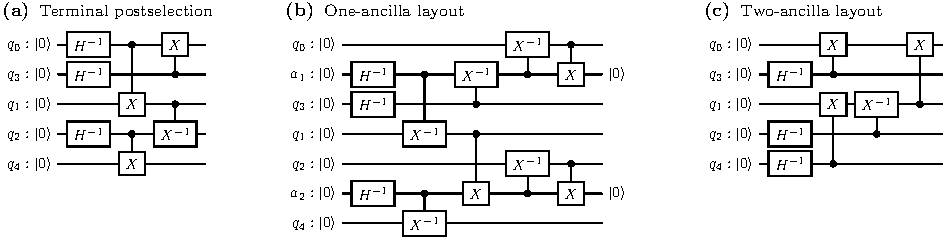
\includegraphics{figures/encoders-three.pdf}% drawn at final size
  \caption{Encoding circuits that prepare $q_0, \dots, q_4$ in $\ket{\bar{+}}$, the $+1$ eigenstate of $\bar X$ (Eq.~\eqref{eq:logicalPauli}), from $\ket{0}$ on every qutrit, in terminal postselection on IQM's Garnet QPU~\cite{IQM240812433} (a) and in the one-ancilla (b) and two-ancilla (c) layouts of \autoref{fig:ancilla_layouts}. Each circuit shows only the qutrits it acts on. $H^{-1}$ and SUM are the gates of Eq.~\eqref{eq:conventions}, and a dot connected to a box $X$ ($X^{-1}$) is a SUM gate (its inverse) with the control on the dot. Every two-qutrit gate acts on a coupling drawn in the matching panel of \autoref{fig:ancilla_layouts}. The rows are ordered so that each column holds one gate moment, a set of gates that act on disjoint qutrits and run in parallel. Counting the moment of the $H^{-1}$ gates, the circuits take three, five and four gate moments and have four, eight and four two-qutrit gates. Since the one-ancilla layout couples no two data qutrits other than $q_2$ and $q_3$, circuit (b) entangles the data through the ancillas $a_1$ and $a_2$, which end in $\ket{0}$. Because the simulations prepare $\ket{\bar{+}}$ without noise (\autoref{sub:noise_models}), their results do not depend on which circuit prepares it.}
  \label{fig:encoding_circuit}
\end{figure*}

% from "method - [[5,1,2]]_3 qutrit surface code.tex", lines 46-68. The table now names the generators; pairs checked by hand from Eqs. (eq:logical_H), (eq:logical_HS) and the rules of Eq. (eq:bg-conjugation).
\autoref{tab:clifford-conjugation} lists how the generators $\bar H$ and $\bar S$ of Eqs.~\eqref{eq:logical_H} and~\eqref{eq:logical_HS} conjugate the stabilizer generators and the logical Pauli operators. Both map the stabilizer group to itself, and they act on $\bar X$ and $\bar Z$ as $H$ and $S$ act on $X$ and $Z$ in Eq.~\eqref{eq:bg-conjugation}.

\begin{table*}[tp]
  \centering
  \begin{tabular}{l|l}
    \hline
    Stabilizer generators & Logical Paulis \\
    \hline
    $\bar H G_1 \bar H^\dagger = G_3^{-1}$, \quad $\bar H G_2 \bar H^\dagger = G_4^{-1}$
      & $\bar H \bar Z \bar H^\dagger = \bar X^{-1}$ \\
    $\bar H G_3 \bar H^\dagger = G_1$, \quad $\bar H G_4 \bar H^\dagger = G_2$
      & $\bar H \bar X \bar H^\dagger = \bar Z$ \\
    $\bar S G_1 \bar S^\dagger = G_1$, \quad $\bar S G_2 \bar S^\dagger = G_2$
      & $\bar S \bar Z \bar S^\dagger = \bar Z$ \\
    $\bar S G_3 \bar S^\dagger = G_3 G_1$, \quad $\bar S G_4 \bar S^\dagger = G_4 G_2$
      & $\bar S \bar X \bar S^\dagger = \bar X \bar Z$ \\
    \hline
  \end{tabular}
  \caption{Conjugation of the stabilizer generators $G_1, \dots, G_4$ (left) and of the logical Pauli operators (right) of the $[[5,1,2]]_3$ code by the logical Clifford generators $\bar H$ and $\bar S$.}
  \label{tab:clifford-conjugation}
\end{table*}

\subsection{Check Round of the One-Ancilla Layout}
\label{app:rounds-one-ancilla}

% from "method - LRB-D.tex", lines 179 (text) and 96-149 (panels (c), (d) of the former protocol figure)
In the one-ancilla layout the ancilla $a_j$ measures $G_j$ with the circuits of \autoref{fig:rounds_one_ancilla}. For the $Z$-type stabilizers $G_1$ and $G_2$, each of the three data qutrits controls a SUM gate or its inverse onto the ancilla, which collects the syndrome in the computational basis. For the $X$-type stabilizers $G_3$ and $G_4$, the ancilla is rotated by $H$, controls a SUM gate or its inverse onto each of the three data qutrits, and is rotated back by $H^{-1}$ before its computational-basis readout. A data qutrit that enters a stabilizer with the exponent $-1$ takes the inverse SUM gate. The round uses all 12 couplings between a site and a neighboring data qutrit, and \autoref{tab:conv_round} lists its gate moments.

\begin{figure*}[tp]
  % from paper-rework/a1-layout-figure/checks-bc.pdf (one-ancilla panels: the five-moment round), caption-checks-bc.tex (restructure 2026-11-19)
  \centering
  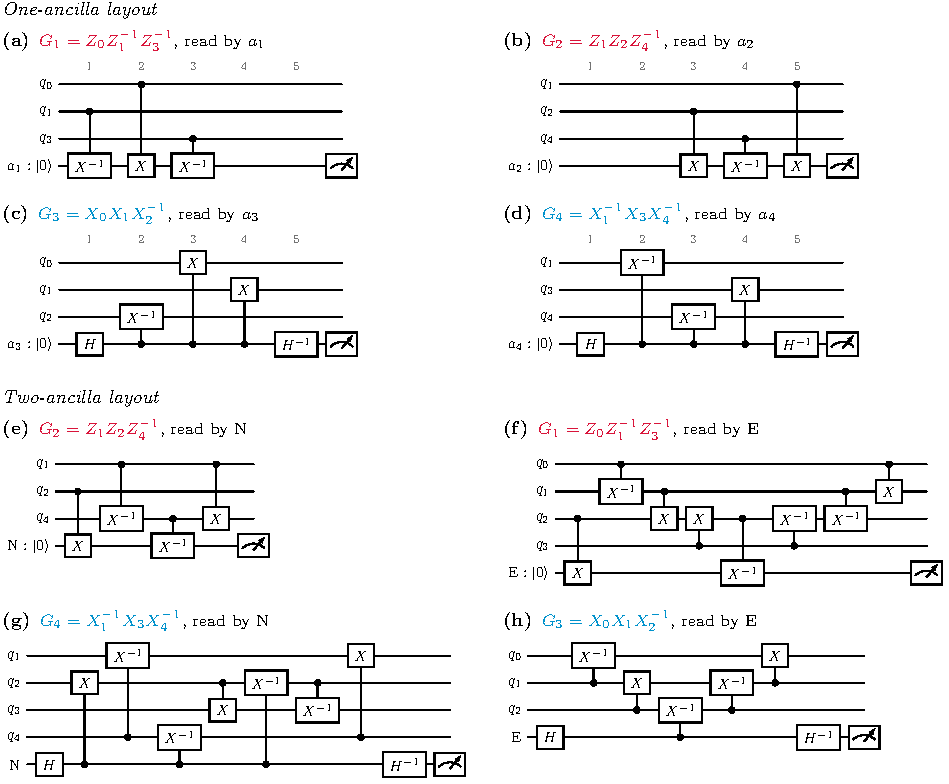
\includegraphics{figures/extraction-two-layouts.pdf}% drawn at final size
  \caption{Syndrome extraction circuits of the two layouts of \autoref{fig:ancilla_layouts}: the one-ancilla layout in (a)--(d) and the two-ancilla layout, with the ancillas N and E, in (e)--(h). Each panel shows only the qutrits it acts on. In (a)--(d) the numbered columns are the gate moments of the round, the time steps in which gates on disjoint qutrits run in parallel, and in (e)--(h) the gates appear in the order in which the round's circuit lists them. The gates are those of Eq.~\eqref{eq:conventions}. A dot connected to a box $X$ ($X^{-1}$) is a SUM gate (its inverse) with the control on the dot, and $\mathrm{SUM}(q_4 \to q_1)$, for example, adds the computational-basis value of the control $q_4$ to the target $q_1$. A data gate is a SUM gate or its inverse between two data qutrits. Let $z_j$ be the computational-basis value of $q_j$, and let the syndrome of $G_j$ be the exponent of $\omega = e^{2\pi i/3}$ in its eigenvalue.
(a)--(d)~Ancilla $a_j$ measures $G_j$ without data gates, with one SUM gate or its inverse per data qutrit of $G_j$, between $H$ and $H^{-1}$ for the $X$-type $G_3$ and $G_4$. The four ancillas are reset to $\ket{0}$ at the start of each check round and read out together at its end. The round runs its 12 two-qutrit and four one-qutrit gates in five gate moments, and an ancilla idles in a moment whose column holds no gate.
(e)--(h)~Panels (e) and (f) form the first half of the round and (g) and (h) the second, with 24 two-qutrit and four one-qutrit gates in all. N and E are reset to $\ket{0}$ at the start of the round, read out at the end of each half and not reset between the halves.
(e)~N adds $z_2$, a data gate sets $q_4$ to $z_4 - z_1$, N subtracts this value, and the data gate is undone, so N holds $z_1 + z_2 - z_4$, the syndrome of $G_2$.
(f)~E adds $z_2$, data gates add $z_1 - z_0 + z_3$ to $q_2$, E subtracts the new value of $q_2$, and the data gates are undone, so E holds $z_0 - z_1 - z_3$, the syndrome of $G_1$.
(g), (h)~Between $H$ and $H^{-1}$ the ancilla controls SUM gates or their inverses onto the data and so collects the eigenvalue of an $X$-type operator. We write each such operator as it acts on the data before the first data gate. In (g), N collects $X_2$ through $q_2$, then $X_1^{-1} X_4^{-1}$ through $q_4$ while $\mathrm{SUM}^{-1}(q_4 \to q_1)$ is in place, and then $X_2^{-1} X_3$ through $q_2$ while $\mathrm{SUM}(q_2 \to q_3)$ is also in place. Their product is $G_4$. In (h), E collects $G_3$ through $q_2$, its only neighbor, while $\mathrm{SUM}^{-1}(q_1 \to q_0)$ and $\mathrm{SUM}(q_2 \to q_1)$ are in place. The data gates are undone before the readout. Because N and E are not reset, the second readout of N is its first readout plus the syndrome of $G_4$, and that of E its first readout plus the syndrome of $G_3$, modulo three.}
  \label{fig:extraction_circuits}\label{fig:rounds_one_ancilla}
\end{figure*}

\subsection{Check Round of the Two-Ancilla Layout}
\label{app:rounds-relay}

% from "method - LRB-D.tex", lines 181-183
In the two-ancilla layout we call the four sites N, W, E and S (\autoref{fig:ancilla_layouts}(c)). N is next to $q_0$, $q_1$ and $q_2$, W to $q_0$, $q_2$ and $q_3$, E to $q_1$, $q_2$ and $q_4$, and S to $q_2$, $q_3$ and $q_4$, so that N can measure $G_3$ and E can measure $G_2$. Another choice of generators would not remove the need for two sites, because the elements of the stabilizer group that could replace $G_1$ or $G_4$ have weight four or five. Nor can the two parts of a boundary stabilizer be read on separate sites and added afterward, because reading a site measures the operator that the site has collected on the data. If N collected $Z_0 Z_1^{-1}$ and E collected $X_1^{-1} X_4^{-1}$, for example, W would read $Z_3^{-1}$ and S would read $X_3$. Every round would then measure $q_3$ in the $Z$ basis and in the $X$ basis, and each of the two readouts would randomize the other.

% from "method - LRB-D.tex", line 183
The data relay instead moves a partial value through a data qutrit, so that one site holds the whole stabilizer before any site is read (\autoref{tab:conv_round}). Let $z_j$ be the computational-basis value of $q_j$, so that the syndrome of $G_1$ is $z_0 - z_1 - z_3$ modulo three. N first measures $G_3$. It then collects $-z_1$ and lends its value to $q_0$ with a SUM gate, which adds this value to that of $q_0$. W collects the value of $q_0$ and $-z_3$. N then takes its value back from $q_0$ and clears the $-z_1$ part against $q_1$. Because N still holds the syndrome of $G_3$ while it lends, W ends with the syndrome of $G_1$ shifted by that of $G_3$. $G_4$ is measured in the same way in the $X$ basis: E collects the part on $q_1$ and lends it to $q_4$, S collects the parts on $q_4$ and $q_3$, and E takes its value back before it measures $G_2$. At the end of the round N holds the syndrome of $G_3$, W that of $G_1$ shifted by the value of N, E that of $G_2$ and S that of $G_4$, each up to a sign. All four readouts are zero exactly when all four syndromes are trivial, so the acceptance rule of \autoref{sub:lrb_d} applies to the readouts unchanged. The round uses 10 of the 12 couplings between a site and a neighboring data qutrit, because W and S never act on $q_2$. As in the one-ancilla round, every two-qutrit gate acts on one ancilla and one data qutrit.

% Moments as scheduled by the production generator: FoldedQutritDetectionCode and FoldedQutritConventionalSitesDetectionCode.conventional_sites_check_round_circuit (conventional-sites worktree, src/lrb/code_definitions.py), scheduled with LRBCircuitGenerator.schedule_moments in paper-rework/scratch/writer-conv/budget.py (budget.out). The column of the one-ancilla round is new (same source).
\begin{table*}[tp]
  \centering
  \footnotesize
  \setlength{\tabcolsep}{4pt}
  \begin{tabular}{c|l|l}
    \hline
    Moment & One-ancilla round & Two-ancilla round \\
    \hline
    1 & $\mathrm{SUM}(q_0 \to a_1)$, $H$ on $a_3$, $a_4$ & $H$ on E, S, N \\
    2 & $\mathrm{SUM}^{-1}(q_1 \to a_1)$, $\mathrm{SUM}(a_3 \to q_0)$ & $\mathrm{SUM}(\mathrm{E} \to q_1)$, $\mathrm{SUM}^{-1}(\mathrm{S} \to q_3)$, $\mathrm{SUM}(\mathrm{N} \to q_0)$ \\
    3 & $\mathrm{SUM}^{-1}(q_3 \to a_1)$, $\mathrm{SUM}(q_1 \to a_2)$ & $\mathrm{SUM}(q_4 \to \mathrm{E})$, $\mathrm{SUM}^{-1}(q_3 \to \mathrm{W})$, $\mathrm{SUM}^{-1}(\mathrm{N} \to q_2)$ \\
    4 & $\mathrm{SUM}(q_2 \to a_2)$, $\mathrm{SUM}(a_3 \to q_1)$, $\mathrm{SUM}(a_4 \to q_3)$ & $\mathrm{SUM}(\mathrm{S} \to q_4)$, $\mathrm{SUM}(\mathrm{N} \to q_1)$ \\
    5 & $\mathrm{SUM}^{-1}(q_4 \to a_2)$, $\mathrm{SUM}^{-1}(a_3 \to q_2)$, $\mathrm{SUM}^{-1}(a_4 \to q_1)$ & $H^{-1}$ on S, N, $\mathrm{SUM}^{-1}(q_4 \to \mathrm{E})$ \\
    6 & $H^{-1}$ on $a_3$, $\mathrm{SUM}^{-1}(a_4 \to q_4)$ & $\mathrm{SUM}^{-1}(\mathrm{E} \to q_1)$ \\
    7 & $H^{-1}$ on $a_4$ & $\mathrm{SUM}^{-1}(q_1 \to \mathrm{N})$, $H^{-1}$ on E \\
    8 & & $\mathrm{SUM}(\mathrm{N} \to q_0)$, $\mathrm{SUM}(q_2 \to \mathrm{E})$ \\
    9 & & $\mathrm{SUM}^{-1}(q_4 \to \mathrm{E})$, $\mathrm{SUM}(q_0 \to \mathrm{W})$ \\
    10 & & $\mathrm{SUM}^{-1}(\mathrm{N} \to q_0)$, $\mathrm{SUM}(q_1 \to \mathrm{E})$ \\
    11 & & $\mathrm{SUM}(q_1 \to \mathrm{N})$ \\
    \hline
  \end{tabular}
  \caption{Gate moments of one check round in the two layouts, as scheduled in the simulations. Each round starts with one moment that resets its four ancillas and ends with one moment that reads them out. $\mathrm{SUM}(a \to b)$ adds the computational-basis value of $a$ to $b$, and $\mathrm{SUM}^{-1}(a \to b)$ subtracts it. For a site in the $X$ basis, between its $H$ and its $H^{-1}$, $\mathrm{SUM}(a \to b)$ instead subtracts the $X$-basis value of $b$ from that of $a$, so that $X$-basis values move against the arrow. In the two-ancilla round, N measures $G_3$ and S measures $G_4$ in moments 1 to 5, while E collects the part on $q_1$, lends it to $q_4$ in moment 3 and takes it back in moment 5. E clears itself against $q_1$ in moment 6 and measures $G_2$ in moments 8 to 10. N collects $-z_1$ in moment 7, lends its value to $q_0$ in moment 8, takes it back in moment 10 and clears itself against $q_1$ in moment 11. W collects $-z_3$ in moment 3 and the value of $q_0$ in moment 9.}
  \label{tab:conv_round}
\end{table*}

% Single-fault enumeration of the two simulated rounds, as the production generator builds them: jpw-review/hw/checks/check_single_faults.py (.out), written by the technical verifier of critic round 1: 1400 and 2072 faults of the noise-model channels, none missed by both rounds and logical; a superset (every one-qutrit Pauli on every wire after every operation, every two-qutrit Pauli after every two-qutrit gate; 2760 and 3816 faults) gives the same result; qubit rounds: 347 and 509 faults, none. The earlier record (LRB-experiment-data-slurm/comparisons/two-ancilla-checks/fault_check.py and CONV-SITES-FACTS.md) covers the one-ancilla round and earlier relay schedules.
\paragraph{Single faults.} We checked by enumeration that neither round lets a single fault through. One Pauli fault is placed in the first of two otherwise noiseless rounds. The fault set contains every channel that the noise models place in a round, at every location and with every Pauli of that channel, which gives $1400$ faults in the one-ancilla round and $2072$ in the two-ancilla round. A fault counts as an undetected logical error if every ancilla readout of both rounds is zero while the error that remains on the data qutrits is a logical operator. The fault set contains no undetected logical error in either layout.

\subsection{Noise Channels and Their Placement}
\label{app:rounds-noise}\label{app:rounds-protocol}

% from "noise models.tex", lines 8-22
The three channels of \autoref{sub:noise_models} act on a state $\rho$ as
\begin{align}
    \mathrm{DEP1}(p)\colon\quad \rho &\mapsto (1-p)\,\rho + \frac{p}{8}\sum_{P \neq I} P \rho\, P^\dagger , \\
    \mathrm{DEP2}(p)\colon\quad \rho &\mapsto (1-p)\,\rho + \frac{p}{80}\sum_{P \neq I \otimes I} P \rho\, P^\dagger ,
    \label{eq:2-depol} \\
    \mathrm{flip}(p)\colon\quad \rho &\mapsto (1-p)\,\rho + \frac{p}{2}\left( X \rho X^\dagger + X^2 \rho\, (X^2)^\dagger \right) ,
    \label{eq:flip-channel}
\end{align}
where $P$ runs over the non-identity Paulis $X^a Z^b$ of one qutrit and over their $80$ non-identity products on two qutrits. The argument is the probability that the channel applies a non-identity Pauli, and every rate of \autoref{tab:circuit-noise} is such a probability. DEP1 is the depolarizing channel of Eq.~\eqref{eq:1-depol} with $p_{\mathrm{mix}} = \tfrac{9}{8}\,p$, because one ninth of the uniform mixture over all nine Paulis reproduces the input state, and DEP2 is the two-qutrit channel $(1-p_{\mathrm{mix}})\,\rho + \tfrac{p_{\mathrm{mix}}}{9} I$ with $p_{\mathrm{mix}} = \tfrac{81}{80}\,p$. The names DEP1 and DEP2 follow~\cite{GidneyHoneycomb2021}, whose classical bit flips on resets and measurements become the flip channel for qutrits. A shift $X^a$ with $a \neq 0$ immediately before a computational-basis measurement changes the recorded outcome by $a$ modulo three.

% from "noise models.tex", lines 26-28, and "method - LRB-D.tex", lines 18 and 22
The channels are placed after the circuit is divided into segments. Each logical Clifford, each check round and each Clifford of the baseline is one segment. Within a segment every gate goes into the earliest moment after the previous operation on each of its qutrits, so that operations on disjoint qutrits run in parallel and the order on each qutrit is kept. A moment holds either gates or resets and measurements, never both. Measurements whose qutrit is not used again in the segment are moved to one final moment, so that all ancilla readouts of a check round share its last moment. An ancilla whose extraction circuit ends earlier idles until then, which accounts for 7 of the 35 idle locations in the gate moments of the one-ancilla round and for 9 of the 57 of the two-ancilla round. No moment spans two segments. The identity element of the Clifford group is applied as an identity gate that occupies one moment and receives the idle noise of a gate moment.

% from "noise models.tex", lines 28 and 50, and the caption of the former table
Every moment then receives the channels of \autoref{tab:circuit-noise} (\autoref{fig:lrb_b} shows an example). The full models contain two further rules, which have no effect in our circuits. The first puts a phase flip, the channel of Eq.~\eqref{eq:flip-channel} with $Z$ and $Z^2$ in place of $X$ and $X^2$, before each $X$-basis measurement, with probability $5p$ under SI1000 and $p$ under SD6. It never applies, because every readout of our circuits is a computational-basis measurement: the $X$-type extraction circuits rotate their ancillas with $H^{-1}$ before the readout. The second puts DEP1 with probability $p$ after each measurement under both models. It acts only on ancillas that are reset before their next use or are not used again, so it changes no detector and no logical outcome. SI1000 requires $p \le 0.2$, so that the probability $5p$ of a measurement flip is at most one.

% from "method - LRB-D.tex", lines 80-94: panel (b) of the former protocol figure, with the matching part of its caption
\begin{figure*}[tp]
    \centering
    \scalebox{0.8}{
    \begin{quantikz}[row sep={0.75cm,between origins}, column sep=0.25cm]
      \lstick{$q_0$} & \gate{S} & \gate{\textcolor{purple}{\mathcal{E}_1}} & \qw \\
      \lstick{$q_1$} & \gate{S^{-1}} & \gate{\textcolor{purple}{\mathcal{E}_1}} & \qw \\
      \lstick{$q_2$} & \ctrl{1} & \gate[2]{\textcolor{purple}{\mathcal{E}_2}} & \qw \\
      \lstick{$q_3$} & \gate{Z} & & \qw \\
      \lstick{$q_4$} & \gate{S} & \gate{\textcolor{purple}{\mathcal{E}_1}} & \qw \\
      \lstick{ancillas} & \qwbundle{n_a} & \gate{\textcolor{purple}{\mathcal{E}_{\mathrm{idle}}}} & \qw
    \end{quantikz}
    }
    \caption{Noise in one segment, here a logical Clifford that consists of $\bar S$ alone and occupies one moment. $\mathcal{E}_1$ is DEP1 after a one-qutrit gate, $\mathcal{E}_2$ is DEP2 after the CZ gate on $q_2$ and $q_3$, and $\mathcal{E}_{\mathrm{idle}}$ is the idle DEP1 on each of the $n_a = 4$ ancillas. $\mathcal{E}_1$ and $\mathcal{E}_{\mathrm{idle}}$ have probability $p/10$ under SI1000 and $p$ under SD6, and $\mathcal{E}_2$ has probability $p$.}
    \label{fig:lrb_b}\label{fig:rounds_segment_noise}
\end{figure*}

\subsection{Deviations from the Reference Models}
\label{app:rounds-deviations}

% from "noise models.tex", lines 52-55
% TODO(authors): confirm that these deviations from the reference noise models are intended (native SUM, CZ and SWAP under both models, no stacking of Idle(p/10) and ResonatorIdle(2p) under SI1000, post-measurement DEP1 in both models).
Our models deviate from those of~\cite{GidneyHoneycomb2021} in three points. First, they contain DEP1 after every measurement, a rule that the reference models lack and that has no effect in our circuits (\appref{app:rounds-noise}). Second, under SI1000 a qutrit that idles in a reset or measurement moment receives DEP1 with probability $2p$ only, whereas in the reference model the rules Idle($p/10$) and ResonatorIdle($2p$) both act on such a qubit. Third, SUM, CZ, their inverses and SWAP are each one native two-qutrit gate followed by DEP2. The reference gate sets contain a single entangling gate, CZ for SI1000 and CNOT for SD6, so that a SWAP or an entangling gate of the other type would there be compiled into several entangling and one-qubit gates.

\subsection{Fault Budgets}
\label{app:rounds-budget}

% Location counts and budgets: paper-rework/scratch/writer-conv/budget.py (budget.out) and jpw-review/hw/checks/check_fault_budgets.py (.out), from the generator of the conventional-sites worktree. Sums: 12 + 0.4 + 8 + 20 + 4 + 3.5 + 20 = 67.9; 18 + 0.6 + 8 + 20 + 4 + 5.7 + 20 = 76.3; 12 + 4 + 4 + 4 + 4 + 35 + 10 = 73; 18 + 6 + 4 + 4 + 4 + 57 + 10 = 103. Logical Clifford: mean over the 216 catalog words, data wires only, 5.73p (SI1000) and 28.78p (SD6); the inverse words give the same means.
\begin{table*}[tp]
  \centering
  \begin{tabular}{l|c|c|c|c|c}
    \hline
    & & \multicolumn{2}{c|}{Locations} & \multicolumn{2}{c}{Probability} \\
    Location & Channel & one-anc. & two-anc. & SI1000 & SD6 \\
    \hline
    Two-qutrit gate & DEP2 & 12 & 18 & $p$ & $p$ \\
    One-qutrit gate & DEP1 & 4 & 6 & $p/10$ & $p$ \\
    Reset & flip & 4 & 4 & $2p$ & $p$ \\
    Measurement, before & flip & 4 & 4 & $5p$ & $p$ \\
    Measurement, after & DEP1 & 4 & 4 & $p$ & $p$ \\
    Idle qutrit in a gate moment & DEP1 & 35 & 57 & $p/10$ & $p$ \\
    Idle qutrit in a reset or measurement moment & DEP1 & 10 & 10 & $2p$ & $p$ \\
    \hline
    Expected number of faults, one-ancilla round & & & & $67.9p$ & $73p$ \\
    Expected number of faults, two-ancilla round & & & & $76.3p$ & $103p$ \\
    \hline
  \end{tabular}
  \caption{Noise locations of one check round in the one-ancilla and in the two-ancilla layout, with the probability of each channel under SI1000 and SD6. The expected number of faults of a round is the sum of the probabilities over its locations.}
  \label{tab:round-budget}
\end{table*}

\autoref{tab:round-budget} derives the expected number of faults of a check round from its noise locations. The count includes the $4p$ of DEP1 after the measurements, which change no detector. The flips on resets and measurements contribute $28p$ of the budget of either round under SI1000 and $8p$ under SD6. The data relay adds $8.4p$ under SI1000, of which $6p$ come from its six two-qutrit gates, $2.2p$ from the 22 idle locations of its four gate moments and $0.2p$ from its two one-qutrit gates. Under SD6 it adds $30p$, of which the same idle locations contribute $22p$.

For a logical Clifford we count the channels on the data qutrits and average over the $216$ words of \appref{sec:clifford-gen}, which gives $5.73p$ under SI1000 and $28.8p$ under SD6. The count leaves out the idle DEP1 on the ancillas during a logical Clifford, because the reset at the start of the next check round erases its effect. One unit of depth holds two logical Cliffords and one check round. Its two Cliffords thus carry $11.5p$ against the $67.9p$ of the one-ancilla round under SI1000, and $57.6p$ against $73p$ under SD6.

\subsection{Qubit Forms of the Channels}
\label{app:rounds-qubit}

% from "method.tex", lines 18-19
% Qubit noise channels: sdim 1.4.0 (N1 'd' uniform over the q^2 - 1 non-identity Paulis, N1 'f'/'p' over the q - 1 nonzero shifts, N2 uniform over the q^4 - 1 non-identity Paulis) and CIRCUIT_LEVEL_NOISE_RATES in src/lrb/circuit_generator.py, identical in the qubit-lrbd-sdim140 and conventional-sites worktrees; mixing forms checked in paper-rework/scratch/corrector-qubit-1/corrector.py (section H)
For the qubit code of \autoref{sub:qubit_code}, DEP1 with probability $p$ applies each of $X$, $Z$ and $XZ$ with probability $p/3$, which is the depolarizing channel with $p_{\mathrm{mix}} = \tfrac{4}{3}\,p$, and DEP2 applies each of the $15$ non-identity two-qubit Paulis with probability $p/15$, which corresponds to $p_{\mathrm{mix}} = \tfrac{16}{15}\,p$. A flip with probability $p$ applies $X$ and inverts the recorded bit. These are the channels of~\cite{GidneyHoneycomb2021} themselves, so the qubit models are the reference models up to the three deviations of \appref{app:rounds-deviations}, with CNOT in place of SUM. The check rounds, their scheduling and the location counts of \autoref{tab:round-budget} are the same as for the qutrit code, and the single-fault enumeration finds no undetected logical error among the $347$ and $509$ faults of the two qubit rounds. A logical Clifford of the qubit code puts $2.80p$ on the data qubits under SI1000 and $14.5p$ under SD6.
 % B (track hw; parked text until M2)

% Appendix C, Simulation Campaign and Fit Details (track sim, 2026-11-13; revised after critic round 1,
% jpw-review/sim/critiques/appCD_critique_round1.md, adjudication in jpw-review/sim/appCD_round1_adjudication.md).
% Written with the journal-paper-writing skill. Sources of the text: jpw-review/handoff/hw-moved-out.tex, Part A
% (blocks A1 to A7, which left the Methods), and the verification detail of the former Results
% (draft/results - circuit-level noise.tex of the 438f6f16 mirror, Secs. 4.1 to 4.7), turned from prose into tables.
% Every number is checked against the data by paper-rework/jpw-review/sim/check_numbers.py: table bodies between
% "BEGIN GEN" and "END GEN" are generated by "check_numbers.py --write" and must not be edited by hand; prose numbers
% are registered in checks_appendix.py under the ids named in the comments below.
\section{Details of the Simulations and of the Fits}\label{app:campaign}

This appendix gives the details behind the estimates of \autoref{sec:method} and the data behind the statements of \autoref{sec:results}: the fits (\appref{app:campaign-fits}), the high-$p$ extension runs and the search for the pseudo-thresholds (\appref{app:campaign-search}), the bootstrap over the random Clifford sequences of \autoref{sub:fit_model} and the comparisons built on it (\appref{app:campaign-bootstrap}), the comparison of runs (\appref{app:campaign-runs}), and the tables behind individual results (\appref{app:campaign-data}). We call that bootstrap the sequence bootstrap. In the tables, ``s.e.'' stands for one standard error of the sequence bootstrap and ``s.d.'' for one standard deviation of the parametric bootstrap; the other symbols are those of \autoref{sec:method} and \autoref{sec:results}.

\subsection{Fits}
\label{app:campaign-fits}

% Finite-shot floor of the modulus (0.886/sqrt(N) for a qutrit, 0.798/sqrt(N) for a qubit): paper-rework/scratch/physics-reviewer-e2/rbfloor.py (.out), scratch/corrector-qubit-1/corrector.py (section G). checks C-floor-*, C-bias-* (facts/raw_per_depth.csv)
This subsection gives six details of the fits: the finite-shot floor of the signals, the number of fitted depths, the weights, the grid of the minimization, the conventions of the error rate and the parametric bootstrap.

The zero offset of Eq.~\eqref{eq:zero_offset_fit} holds for the expectation value of the estimate and not for its modulus at a finite number of shots. For $N$ shots with uniformly random outcomes the modulus averages about $0.9/\sqrt{N}$ for a qutrit and $0.8/\sqrt{N}$ for a qubit, which we call the finite-shot floor. The data reach it in three places. The physical signal under SD6, with $10^4$ shots per sequence, levels off at $0.007$ to $0.010$, around its floor of $0.009$, from $m = 18$ on for $p \ge 0.03$ and at $m = 22$ for $p = 0.02$ in the production runs of both layouts, while under SI1000 it stays above $0.27$. LRB-D points with few accepted shots are biased upward in the same way: in the production run of the one-ancilla layout under SD6 with $k = 4$ at $p = 0.02$, the point at $m = 10$ rests on an average of $3.6$ accepted shots per sequence and reads $\langle \bar{X} \rangle = 0.55$, above the value $0.39$ at $m = 2$, and in the SD6 extension run of the same layout at $p = 0.035$ and $k = 1$ the point at $m = 4$, with $3.8$ accepted shots per sequence, reads $0.68$, above $0.21$ at $m = 3$. Under terminal postselection, at $m = 22$ and $p \ge 0.02$ under SD6, the accepted logical signal and the physical signal have both reached their floors (\autoref{tab:const0}).

% Number of fitted depths: generated table k1_depths (facts/fits_all_k.csv); check C-two-depths, C-zero-fit
The depth rule of \autoref{sub:fit_model} leaves fewer depths as $p$ grows (\autoref{tab:k1_depths}). An LRB-D fit needs at least two depths, and the baseline fits use every depth of their run. A fit over two depths passes through both points, unless the second lies above the first, in which case $f$ is capped at one and the fit returns zero error (footnote of \autoref{tab:overlap}). Either way it carries no information on the shape of the decay, and its bootstrap interval reflects only the statistical errors of the two points. Fits over two depths occur in the production runs with $k = 1$ from $p = 0.04$ on under SI1000 and from $p = 0.03$ on under SD6.

\begin{table*}[tp]
  \centering
  \small
  \begin{tabular}{c|cc|cc|cc|cc}
    \hline
    & \multicolumn{4}{c|}{one-ancilla layout} & \multicolumn{4}{c}{two-ancilla layout} \\
    & \multicolumn{2}{c|}{SI1000} & \multicolumn{2}{c|}{SD6} & \multicolumn{2}{c|}{SI1000} & \multicolumn{2}{c}{SD6} \\
    $p$ & $n$ & $\chi^2/(n-2)$ & $n$ & $\chi^2/(n-2)$ & $n$ & $\chi^2/(n-2)$ & $n$ & $\chi^2/(n-2)$ \\
    \hline
    % BEGIN GEN k1_depths
    0.001 & 9 & 0.04 & 9 & 0.94 & 9 & 0.03 & 9 & 0.32 \\
    0.002 & 9 & 0.01 & 9 & 2.15 & 9 & 0.03 & 9 & 0.65 \\
    0.005 & 9 & 0.06 & 8 & 0.81 & 9 & 0.10 & 6 & 0.16 \\
    0.0075 & 8 & 0.07 & 5 & 0.62 & 8 & 0.28 & 5 & 0.17 \\
    0.01 & 6 & 0.06 & 5 & 0.51 & 6 & 0.08 & 4 & 0.14 \\
    0.0125 & 5 & 0.01 & 4 & 0.66 & 5 & 0.09 & 4 & 0.13 \\
    0.015 & 4 & 0.08 & 4 & 0.25 & 4 & 0.06 & 3 & 0.04 \\
    0.02 & 4 & 0.01 & 3 & 0.09 & 4 & 0.07 & 3 & 0.47 \\
    0.03 & 3 & 0.00 & 2 & -- & 3 & 0.07 & 2 & -- \\
    0.04 & 2 & -- & 2 & -- & 2 & -- & 2 & -- \\
    0.05 & 2 & -- & 2 & -- & 2 & -- & 2 & -- \\
    % END GEN k1_depths
    \hline
  \end{tabular}
  \caption{LRB-D fits of the production runs of the $[[5,1,2]]_3$ code for $k = 1$, at the grid points from $p = 10^{-3}$ on: number $n$ of fitted depths and $\chi^2$ per degree of freedom (\autoref{sub:fit_model}), which is not defined for $n = 2$.}
  \label{tab:k1_depths}
\end{table*}

% Weights of the fit: _safe_weights in src/lrb/lrb_plotting.py (np.std with ddof = 0 in src/lrb/lrb_simulation.py); checks C-w-A, C-w-sigma0, C-w-share (facts/fits_all_k.csv, raw_per_depth.csv)
The weights $1/\sigma_m^2$ of the fit use the population standard deviation $\sigma_m$ of the per-sequence moduli, with divisor $N_s$. A depth with $\sigma_m = 0$ receives $10^{-3}$ times the median of the $\sigma_m$ over the fitted depths in place of zero. For the baseline at $m = 0$ (\autoref{sub:fit_model}) this replacement holds the amplitude at $A = 1$ to within $3\times10^{-8}$, so the baseline fit is in effect $f^m$. For LRB-D the circuits of depth zero are the same for all sequences of a run, so $\sigma_0$ contains shot noise only, and depth zero carries more than half of the total weight in two thirds of the production fits of the qutrit code with $k \le 4$. At the other end, a largest fitted depth with few accepted shots, such as those of the bracketing fits of \appref{app:campaign-search}, carries little weight, because its scatter over the sequences is large: in the extension run of the one-ancilla layout under SI1000 at $p = 0.03$ and $k = 1$, the signal at $m = 6$ scatters over the sequences with a standard deviation of $0.23$, against $0.005$ to $0.03$ at $m = 1$ to $4$.

% Grid of the fit: _fit_decay_parameter_fixed_a in src/lrb/lrb_plotting.py; checks C-w-step, C-w-step1, C-w-min
The fit minimizes over a grid in $f$ that is refined to a spacing of $8\times10^{-7}$, or $5\times10^{-8}$ next to $f = 1$. The smallest nonzero fitted error rate of the qutrit code, $3.3\times10^{-8}$ for LRB-D in the one-ancilla layout under SI1000 at $p = 10^{-4}$ and $k = 1$, corresponds to one such spacing, so error rates of this size are not resolved, and a fit that lands on $f = 1$ returns zero error (\autoref{fig:four_configs}, \autoref{fig:k1_qubit_qutrit}).

Two conventions enter the error rate $r$ of \autoref{sub:fit_model}, the unit of depth and the factor $(q-1)/q$, and neither changes a pseudo-threshold. Per Clifford instead of per unit of depth, the decay parameter would be $f^{1/2}$, with an error rate close to $r/2$ when $r$ is small. Because $r$ decreases monotonically with $f$, the condition $r_{\mathrm{LRB}} = r_{\mathrm{RB}}$ that defines $p^\star(k)$ is equivalent to $f_{\mathrm{LRB}} = f_{\mathrm{RB}}$ and to $f_{\mathrm{LRB}}^{1/2} = f_{\mathrm{RB}}^{1/2}$, and the factor $(q-1)/q$ drops out, since $p^\star$ compares two error rates of the same local dimension. The ratios of \autoref{tab:rb_ratio} and \autoref{tab:lrb_ratio}, which \autoref{sub:qubit_comparison} quotes, compare error rates of different local dimension and would be larger by a factor of $4/3$ in terms of $1 - f$, which does not change their direction.

% Parametric bootstrap: _bootstrap_error_rates in src/lrb/lrb_plotting.py (500 replicates)
For the parametric bootstrap of a fitted error rate, we perturb every sequence-averaged point by Gaussian noise whose width is its standard error over the sequences, clip the point to $[0, 1]$, refit with Eq.~\eqref{eq:zero_offset_fit} and the same weights, and repeat this $500$ times. The depths move together under another draw of sequences (\autoref{sub:fit_model}) because all depths of a sequence share its first Cliffords.

\subsection{Extension Runs and Pseudo-Threshold Search}
\label{app:campaign-search}

% checks C-prod-* (facts/raw_per_depth.csv, 1anc-si1000, unif-1, p = 0.03)
This subsection gives why the high-$p$ extension runs are needed, which depths they fit, the search rule and the fits that bracket each pseudo-threshold. Near the pseudo-thresholds the production runs lose the depths that the extension runs restore (\autoref{sub:sim_framework}): in the production run of the one-ancilla layout under SI1000 at $p = 0.03$ and $k = 1$, the postselection rejects $77\%$ of the shots at $m = 0$ and $99.74\%$ at $m = 2$, an average of $28$ of $10^6$ shots per sequence is accepted at $m = 4$, and from $m = 6$ on at least one sequence has no accepted shot. The extension run restores the depths up to $m = 6$ there (\autoref{tab:brackets}).

% Even-depth rule: applied by scripts/merge_highp_threshold_extension.py (class EvenDepthsForSparseChecks); checks C-step-* (facts/raw_per_depth.csv, 1anc-sd6, unif-3, p = 1e-3)
The extension fits for $k \ge 2$ use only even depths so that they hold the same depths modulo two as the production fits, whose depths are all even. The parity matters because the accepted logical signal steps at depths that are not multiples of $k$: there the last $m \bmod k$ forward Cliffords are followed by check rounds outside the postselection, so the signal lies on a different curve than at the multiples of $k$. In the production run of the one-ancilla layout under SD6 at $p = 10^{-3}$ and $k = 3$, $\langle \bar{X} \rangle$ drops by $1.8\times10^{-4}$ from $m = 14$ to $18$, where $m \bmod 3$ falls from 2 to 0, and by $2.2\times10^{-3}$ from $m = 18$ to $20$, where it rises to 2, while the standard errors of these points are $0.8\times10^{-4}$ to $1.6\times10^{-4}$. The same steps appear near the SI1000 pseudo-thresholds: in the extension run of the one-ancilla layout at $p = 0.015$ and $k = 3$, $\langle \bar{X} \rangle$ rises from $0.864$ at $m = 2$ to $0.880$ at $m = 3$, by eleven standard errors. For $k = 2$ the rule removes every such depth of the extension runs, $m = 1$ and $3$. For $k = 3$ it also removes the multiple $m = 3$, and for $k = 3$ and $4$ the even depths still include depths that are not multiples of $k$, in the extension runs ($m = 2$ and $4$ for $k = 3$, $m = 2$ and $6$ for $k = 4$) as in the production runs. The steps raise $\chi^2$ per degree of freedom of the SI1000 production fits for $k = 3$ and $4$ (\autoref{tab:kdep}).

% Search rule: plot_all_unif_threshold_graphs in src/lrb/lrb_plotting.py, reimplemented in scratch/writer-qubit/qlib.py (threshold, tail_cut); checks C-search-*
The search for $p^\star(k)$ runs on a merged grid, for the qutrit code the one of \autoref{sub:sim_framework} and \autoref{fig:threshold_grid_si1000_1anc}. For the qubit code it holds the refinement fits inside the range of the refinement run (\autoref{tab:runs}) and the production fits outside it. We take $p^\star(k)$ at the onset of the range in which $r_{\mathrm{LRB}}$ stays at or above $r_{\mathrm{RB}}$ at every larger $p$ of the grid; the interpolation of \autoref{sub:fit_model} runs between the onset and the grid point below it. The search skips the three lowest grid points. The qutrit search adds two conditions. A tolerance of $5\times10^{-4}$ counts $r_{\mathrm{LRB}}$ as at or above $r_{\mathrm{RB}}$ when it lies below it by less than this amount; if the difference then has the same sign at the onset and at the point below it, the search returns the onset itself. An error floor of $2\times10^{-3}$ removes from the search every grid point below the first one at which $r_{\mathrm{LRB}}$ or $r_{\mathrm{RB}}$ reaches this value. Before either search, the grid is cut at the first point beyond its first six where $r_{\mathrm{LRB}}$ or $r_{\mathrm{RB}}$ drops below its running maximum by more than $0.01$ or $25\%$, whichever is larger; the cut guards against LRB-D fits with too few accepted shots. On the merged grids of all sixteen qutrit and all sixteen qubit pseudo-thresholds, this cut removes no point.

% Bracketing fits: generated tables brackets and brackets_rates (refits with qlib.py; canonical p* from comparisons/pseudo-thresholds-current.csv, one-ancilla rows, and pseudo-thresholds-conv-sites-current.csv); checks C-br-*
\autoref{tab:brackets} lists the two fits that bracket each pseudo-threshold, and \autoref{tab:brackets_rates} their error rates and fit quality. Five values lie between two production points, the SD6 values for $k = 3$ and $4$ in both layouts and the SI1000 value for $k = 4$ in the two-ancilla layout, and there the extension runs only confirm that $r_{\mathrm{LRB}}$ stays above $r_{\mathrm{RB}}$ at larger $p$.

\begin{table*}[tp]
  \centering
  \footnotesize
  \setlength{\tabcolsep}{4pt}
  \begin{tabular}{llc|ccccc|ccccc}
    \hline
    & & & \multicolumn{5}{c|}{fit below $p^\star(k)$} & \multicolumn{5}{c}{fit above $p^\star(k)$} \\
    layout & model & $k$ & $p$ & run & $n$ & $m_{\max}$ & shots & $p$ & run & $n$ & $m_{\max}$ & shots \\
    \hline
    % BEGIN GEN brackets
    one-ancilla & SI1000 & 1 & 0.0275 & E & 6 & 6 & 22.8 & 0.03 & E & 6 & 6 & 6.7 \\
     &  & 2 & 0.0225 & E & 4 & 6 & 2321 & 0.025 & E & 4 & 6 & 887 \\
     &  & 3 & 0.015 & E & 4 & 6 & $7.4\times10^{4}$ & 0.0175 & E & 4 & 6 & $3.0\times10^{4}$ \\
     &  & 4 & 0.0125 & P & 7 & 18 & 7.2 & 0.015 & E & 4 & 6 & $1.3\times10^{5}$ \\
    \hline
     & SD6 & 1 & 0.035 & E & 5 & 4 & 3.8 & 0.04 & E & 4 & 3 & 32.1 \\
     &  & 2 & 0.025 & E & 4 & 6 & 10.7 & 0.03 & E & 3 & 4 & 186 \\
     &  & 3 & 0.015 & P & 4 & 6 & 105 & 0.02 & P & 4 & 6 & 13.7 \\
     &  & 4 & 0.015 & P & 5 & 10 & 7.5 & 0.02 & P & 5 & 10 & 3.6 \\
    \hline
    two-ancilla & SI1000 & 1 & 0.025 & E & 6 & 6 & 19.5 & 0.0275 & E & 5 & 4 & 482 \\
     &  & 2 & 0.02 & E & 4 & 6 & 2294 & 0.0225 & E & 4 & 6 & 774 \\
     &  & 3 & 0.0125 & P & 6 & 14 & 16.3 & 0.015 & E & 4 & 6 & $3.6\times10^{4}$ \\
     &  & 4 & 0.01 & P & 8 & 20 & 4.8 & 0.0125 & P & 6 & 14 & 24.3 \\
    \hline
     & SD6 & 1 & 0.025 & E & 5 & 4 & 7.4 & 0.03 & E & 4 & 3 & 31.8 \\
     &  & 2 & 0.02 & P & 3 & 4 & 23.0 & 0.025 & E & 3 & 4 & 114 \\
     &  & 3 & 0.01 & P & 4 & 6 & 298 & 0.0125 & P & 4 & 6 & 57.4 \\
     &  & 4 & 0.01 & P & 5 & 10 & 15.2 & 0.0125 & P & 4 & 6 & 337 \\
    % END GEN brackets
    \hline
  \end{tabular}
  \caption{The two LRB-D fits that bracket each pseudo-threshold of \autoref{tab:pseudo_thresholds}: the grid point $p$, the run that supplies the fit (P for production, E for high-$p$ extension), the number $n$ of fitted depths, the largest fitted depth $m_{\max}$ and the number of accepted shots per sequence at that depth, averaged over the sequences. On the grid of $p$ that merges the runs (\appref{app:campaign-search}), $r_{\mathrm{LRB}} - r_{\mathrm{RB}}$ changes sign only between the two points listed.}
  \label{tab:brackets}
\end{table*}

\begin{table*}[tp]
  \centering
  \footnotesize
  \setlength{\tabcolsep}{4pt}
  \begin{tabular}{llc|ccc|ccc}
    \hline
    & & & \multicolumn{3}{c|}{fit below $p^\star(k)$} & \multicolumn{3}{c}{fit above $p^\star(k)$} \\
    layout & model & $k$ & $r_{\mathrm{LRB}}$ & $r_{\mathrm{RB}}$ & $\chi^2/(n-2)$ & $r_{\mathrm{LRB}}$ & $r_{\mathrm{RB}}$ & $\chi^2/(n-2)$ \\
    \hline
    % BEGIN GEN brackets_rates
    one-ancilla & SI1000 & 1 & 0.0172 & 0.0200 & 0.30 & 0.0231 & 0.0217 & 0.32 \\
     &  & 2 & 0.0145 & 0.0165 & 0.32 & 0.0198 & 0.0182 & 0.34 \\
     &  & 3 & 0.0090 & 0.0110 & 5.38 & 0.0140 & 0.0128 & 5.52 \\
     &  & 4 & 0.0084 & 0.0095 & 3.42 & 0.0137 & 0.0110 & 5.36 \\
    \hline
     & SD6 & 1 & 0.1734 & 0.2092 & 1.35 & 0.2351 & 0.2341 & 0.26 \\
     &  & 2 & 0.1328 & 0.1573 & 0.75 & 0.2244 & 0.1837 & 0.24 \\
     &  & 3 & 0.0722 & 0.1102 & 0.30 & 0.1643 & 0.1403 & 0.86 \\
     &  & 4 & 0.1025 & 0.1102 & 2.49 & 0.2062 & 0.1403 & 1.31 \\
    \hline
    two-ancilla & SI1000 & 1 & 0.0169 & 0.0196 & 0.39 & 0.0228 & 0.0213 & 0.54 \\
     &  & 2 & 0.0142 & 0.0156 & 0.46 & 0.0200 & 0.0175 & 0.37 \\
     &  & 3 & 0.0081 & 0.0094 & 4.79 & 0.0133 & 0.0118 & 8.90 \\
     &  & 4 & 0.0063 & 0.0075 & 3.12 & 0.0118 & 0.0094 & 4.42 \\
    \hline
     & SD6 & 1 & 0.1358 & 0.1715 & 0.43 & 0.2187 & 0.2002 & 0.31 \\
     &  & 2 & 0.1130 & 0.1330 & 0.01 & 0.2356 & 0.1715 & 0.00 \\
     &  & 3 & 0.0447 & 0.0715 & 0.85 & 0.0918 & 0.0885 & 0.74 \\
     &  & 4 & 0.0634 & 0.0715 & 1.58 & 0.1390 & 0.0885 & 2.14 \\
    % END GEN brackets_rates
    \hline
  \end{tabular}
  \caption{The bracketing fits of \autoref{tab:brackets}: fitted error rates per unit of depth of LRB-D and of the baseline at the two grid points, and $\chi^2$ per degree of freedom of the LRB-D fit (\autoref{sub:fit_model}).}
  \label{tab:brackets_rates}
\end{table*}


% Qubit search (SCALE_FREE_THRESHOLD_CONFIG: tolerance 0, no error floor) and its sensitivity: scratch/writer-qubit/qlib.py; checks C-qs-*; bracketing fits: generated table brackets_qubit
The qubit search omits the tolerance and the error floor, so the qubit $p^\star(k)$ is the crossing itself (\autoref{tab:brackets_qubit}, \autoref{tab:brackets_rates_qubit}). The two conditions carry absolute values, at most a quarter of the qutrit error rates at the crossings, which are $8.2\times10^{-3}$ to $0.021$ per unit of depth under SI1000 and $0.074$ to $0.23$ under SD6, but comparable to the qubit error rates at the SI1000 crossings, $1.0\times10^{-3}$ to $3.9\times10^{-3}$; under SD6 the qubit error rates at the crossings are $1.6\times10^{-2}$ to $6.8\times10^{-2}$.

\begin{table*}[tp]
  \centering
  \footnotesize
  \setlength{\tabcolsep}{4pt}
  \begin{tabular}{llc|cccc|cccc}
    \hline
    & & & \multicolumn{4}{c|}{fit below $p^\star(k)$} & \multicolumn{4}{c}{fit above $p^\star(k)$} \\
    layout & model & $k$ & $p$ & $n$ & $m_{\max}$ & shots & $p$ & $n$ & $m_{\max}$ & shots \\
    \hline
    % BEGIN GEN brackets_qubit
    one-ancilla & SI1000 & 1 & 0.011 & 6 & 14 & 16.9 & 0.0115 & 6 & 14 & 10.7 \\
     &  & 2 & 0.0075 & 9 & 22 & 120 & 0.008 & 9 & 22 & 66.8 \\
     &  & 3 & 0.0045 & 9 & 22 & 7605 & 0.005 & 9 & 22 & 4497 \\
     &  & 4 & 0.0035 & 9 & 22 & $2.8\times10^{4}$ & 0.004 & 9 & 22 & $1.7\times10^{4}$ \\
    \hline
     & SD6 & 1 & 0.021 & 4 & 6 & 16.3 & 0.022 & 3 & 4 & 337 \\
     &  & 2 & 0.015 & 5 & 10 & 14.2 & 0.016 & 5 & 10 & 9.4 \\
     &  & 3 & 0.009 & 8 & 20 & 6.3 & 0.01 & 6 & 14 & 95.0 \\
     &  & 4 & 0.007 & 9 & 22 & 32.4 & 0.008 & 9 & 22 & 12.3 \\
    \hline
    two-ancilla & SI1000 & 1 & 0.009 & 6 & 14 & 41.2 & 0.0095 & 6 & 14 & 22.3 \\
     &  & 2 & 0.006 & 9 & 22 & 264 & 0.0065 & 9 & 22 & 134 \\
     &  & 3 & 0.0035 & 9 & 22 & $1.3\times10^{4}$ & 0.004 & 9 & 22 & 6797 \\
     &  & 4 & 0.003 & 9 & 22 & $2.9\times10^{4}$ & 0.0035 & 9 & 22 & $1.6\times10^{4}$ \\
    \hline
     & SD6 & 1 & 0.014 & 4 & 6 & 45.7 & 0.015 & 4 & 6 & 25.3 \\
     &  & 2 & 0.01 & 5 & 10 & 36.0 & 0.011 & 5 & 10 & 15.9 \\
     &  & 3 & 0.006 & 8 & 20 & 14.3 & 0.007 & 8 & 20 & 3.6 \\
     &  & 4 & 0.0045 & 9 & 22 & 96.4 & 0.005 & 9 & 22 & 43.5 \\
    % END GEN brackets_qubit
    \hline
  \end{tabular}
  \caption{The two LRB-D fits that bracket each pseudo-threshold of the qubit code (\autoref{tab:pseudo_thresholds_qubit}): the grid point $p$, the number $n$ of fitted depths, the largest fitted depth $m_{\max}$ and the number of accepted shots per sequence at that depth, averaged over the sequences. All fits come from the refinement runs. On the grid of $p$ that merges the runs (\appref{app:campaign-search}), $r_{\mathrm{LRB}} - r_{\mathrm{RB}}$ changes sign only between the two points listed.}
  \label{tab:brackets_qubit}
\end{table*}
\begin{table*}[tp]
  \centering
  \footnotesize
  \setlength{\tabcolsep}{4pt}
  \begin{tabular}{llc|ccc|ccc}
    \hline
    & & & \multicolumn{3}{c|}{fit below $p^\star(k)$} & \multicolumn{3}{c}{fit above $p^\star(k)$} \\
    layout & model & $k$ & $r_{\mathrm{LRB}}$ & $r_{\mathrm{RB}}$ & $\chi^2/(n-2)$ & $r_{\mathrm{LRB}}$ & $r_{\mathrm{RB}}$ & $\chi^2/(n-2)$ \\
    \hline
    % BEGIN GEN brackets_rates_qubit
    one-ancilla & SI1000 & 1 & 0.00365 & 0.00381 & 0.18 & 0.00422 & 0.00399 & 0.15 \\
     &  & 2 & 0.00249 & 0.00261 & 0.03 & 0.00289 & 0.00280 & 0.05 \\
     &  & 3 & 0.00135 & 0.00157 & 1.77 & 0.00177 & 0.00174 & 2.04 \\
     &  & 4 & 0.00105 & 0.00121 & 0.96 & 0.00141 & 0.00140 & 1.27 \\
    \hline
     & SD6 & 1 & 0.06815 & 0.06817 & 0.05 & 0.07680 & 0.07063 & 0.18 \\
     &  & 2 & 0.04934 & 0.04963 & 0.46 & 0.05738 & 0.05277 & 0.43 \\
     &  & 3 & 0.02875 & 0.03041 & 0.72 & 0.03671 & 0.03367 & 0.85 \\
     &  & 4 & 0.02293 & 0.02385 & 1.58 & 0.03027 & 0.02712 & 1.21 \\
    \hline
    two-ancilla & SI1000 & 1 & 0.00275 & 0.00295 & 0.18 & 0.00326 & 0.00314 & 0.14 \\
     &  & 2 & 0.00183 & 0.00199 & 0.04 & 0.00219 & 0.00215 & 0.06 \\
     &  & 3 & 0.00099 & 0.00116 & 2.30 & 0.00134 & 0.00132 & 2.28 \\
     &  & 4 & 0.00094 & 0.00099 & 1.23 & 0.00132 & 0.00116 & 1.32 \\
    \hline
     & SD6 & 1 & 0.04476 & 0.04578 & 0.01 & 0.05347 & 0.04917 & 0.01 \\
     &  & 2 & 0.03332 & 0.03334 & 0.36 & 0.04190 & 0.03650 & 0.31 \\
     &  & 3 & 0.01975 & 0.02018 & 0.95 & 0.02820 & 0.02360 & 0.89 \\
     &  & 4 & 0.01429 & 0.01523 & 1.66 & 0.01849 & 0.01693 & 1.66 \\
    % END GEN brackets_rates_qubit
    \hline
  \end{tabular}
  \caption{The bracketing fits of \autoref{tab:brackets_qubit}: fitted error rates per unit of depth of LRB-D and of the baseline at the two grid points, and $\chi^2$ per degree of freedom of the LRB-D fit (\autoref{sub:fit_model}).}
  \label{tab:brackets_rates_qubit}
\end{table*}

\subsection{Sequence Bootstrap and Comparisons}
\label{app:campaign-bootstrap}

% Sequence bootstrap of the pseudo-thresholds: scripts/sequence_bootstrap_thresholds.py, outputs in LRB-experiment-data-slurm/comparisons/sequence-bootstrap/ (seq_boot_se copied to the canonical files); seq_boot_valid_fraction = 1.0 for all entries; check C-boot-valid
The standard errors of the pseudo-thresholds (\autoref{sub:fit_model}) come from the sequence bootstrap, which has $1000$ replicates. Each replicate draws 30 sequences with replacement from the 30 sequences of a set and applies this draw to every depth and every $p$ of that set. The four sets behind a pseudo-threshold, those of LRB-D and of the baseline in the production run and in the extension or refinement run, are resampled independently. From the outcome counts of the drawn sequences we rebuild the sequence averages and their spread at every depth, refit every decay, with the depth rule of \autoref{sub:fit_model} applied to the drawn sequences, and repeat the search, cut included. The standard error is the standard deviation of $p^\star(k)$ over the replicates, and every replicate finds a crossing. The outcomes of the individual baseline sequences were not stored. We therefore simulate the stored baseline circuits again, with $10^4$ new shots per sequence and depth as for the stored baselines, and in each replicate we shift the fitted baseline error rate of the run by the change that the resampling produces in the fit to the new data.

% Paired adjacent-interval steps and fall factors: sequence-bootstrap replicate files (generated table fall_factors); ratios between runs: generated tables model_ratio, qubit_layout_gap
How two pseudo-thresholds are compared depends on whether they share sequences. The four intervals of one layout and noise model do, so we evaluate their differences and ratios replicate by replicate (\autoref{tab:fall_factors}). The layout gaps at different intervals share the sequences of both runs as well; their differences cannot be judged from the tabulated standard errors, and we have not tested whether the gap changes with $k$. Pseudo-thresholds of different layouts, noise models or codes come from independent runs. We compare two of them through their ratio, whose relative standard error is the two relative standard errors added in quadrature, and we quote the difference of the ratio from one in units of this standard error (\autoref{tab:model_ratio}, \autoref{tab:qubit_layout_gap}).

\begin{table*}[tp]
  \centering
  \small
  \begin{tabular}{ll|cc|cc|c}
    \hline
    & & \multicolumn{2}{c|}{qutrit code} & \multicolumn{2}{c|}{qubit code} & qubit against \\
    layout & model & $p^\star(1)/p^\star(4)$ & step (s.e.) & $p^\star(1)/p^\star(4)$ & step (s.e.) & qutrit (s.e.) \\
    \hline
    % BEGIN GEN fall_factors
    one-ancilla & SI1000 & $2.21 \pm 0.04$ & 8.0 & $2.84 \pm 0.05$ & 18.7 & 8.6 \\
     & SD6 & $2.57 \pm 0.12$ & 6.1 & $2.91 \pm 0.08$ & 12.1 & 2.2 \\
    two-ancilla & SI1000 & $2.45 \pm 0.05$ & 9.4 & $2.98 \pm 0.04$ & 16.1 & 7.0 \\
     & SD6 & $2.74 \pm 0.08$ & 6.6 & $3.03 \pm 0.06$ & 18.2 & 2.9 \\
    % END GEN fall_factors
    \hline
  \end{tabular}
  \caption{Fall of the pseudo-threshold with the interval. For each code: the factor $p^\star(1)/p^\star(4)$ with its standard error over the replicates of the sequence bootstrap, and, in the columns ``step'', the smallest of the three differences $p^\star(k) - p^\star(k+1)$ in units of its standard error (s.e.), both evaluated replicate by replicate. Last column: the difference of the ratio of the qubit to the qutrit factor from one, in units of the standard error of this ratio. In all 1000 replicates of every row and code, $p^\star(1) > p^\star(2) > p^\star(3) > p^\star(4)$.}
  \label{tab:fall_factors}
\end{table*}

\begin{table*}[tp]
  \centering
  \small
  \begin{tabular}{c|cc|cc|cc}
    \hline
    & \multicolumn{2}{c|}{one-ancilla layout} & \multicolumn{2}{c|}{two-ancilla layout} & \multicolumn{2}{c}{layout gap, SD6 minus SI1000} \\
    $k$ & difference (\%) & in s.e. & difference (\%) & in s.e. & difference (points) & in s.e. \\
    \hline
    % BEGIN GEN model_ratio
    1 & $+36.7 \pm 5.7$ & 6.5 & $+6.4 \pm 3.1$ & 2.0 & $20.2 \pm 3.9$ & 5.2 \\
    2 & $+12.6 \pm 3.7$ & 3.4 & $+1.5 \pm 2.1$ & 0.7 & $8.6 \pm 3.2$ & 2.7 \\
    3 & $+8.8 \pm 4.5$ & 1.9 & $-10.4 \pm 3.1$ & 3.3 & $14.5 \pm 4.0$ & 3.6 \\
    4 & $+17.6 \pm 3.8$ & 4.6 & $-4.6 \pm 1.8$ & 2.6 & $15.5 \pm 2.7$ & 5.8 \\
    % END GEN model_ratio
    \hline
  \end{tabular}
  \caption{The two noise models compared. For each layout: the relative difference $p^\star_{\mathrm{SD6}}/p^\star_{\mathrm{SI1000}} - 1$ of the pseudo-thresholds of the qutrit code in percent, with one standard error, and its size in units of this standard error (s.e.). Last two columns: the layout gap of \autoref{tab:pseudo_thresholds} under SD6 minus that under SI1000, in percentage points, with its standard error, for which the standard errors of the two gaps are added in quadrature.}
  \label{tab:model_ratio}
\end{table*}

\begin{table*}[tp]
  \centering
  \small
  \begin{tabular}{c|cc|cc}
    \hline
    & \multicolumn{2}{c|}{SI1000} & \multicolumn{2}{c}{SD6} \\
    $k$ & gap (\%) & in s.e. & gap (\%) & in s.e. \\
    \hline
    % BEGIN GEN qubit_layout_gap
    1 & $16.9 \pm 2.0$ & 8.4 & $32.4 \pm 3.3$ & 9.9 \\
    2 & $17.5 \pm 2.2$ & 7.9 & $33.6 \pm 2.7$ & 12.3 \\
    3 & $20.1 \pm 2.1$ & 9.6 & $35.0 \pm 2.8$ & 12.6 \\
    4 & $20.9 \pm 2.1$ & 10.1 & $35.1 \pm 2.8$ & 12.4 \\
    % END GEN qubit_layout_gap
    \hline
  \end{tabular}
  \caption{Layout gap $1 - p^\star_{\mathrm{two}}/p^\star_{\mathrm{one}}$ of the qubit code in percent, from the values of \autoref{tab:pseudo_thresholds_qubit}, with one standard error, and its size in units of this standard error (s.e.).}
  \label{tab:qubit_layout_gap}
\end{table*}

\subsection{Comparison of Runs}
\label{app:campaign-runs}

% Baselines of different runs and word lengths (gate tokens per Clifford in the RB circuits): generated table rb_layouts; earlier check: scratch/writer-conv/analysis.py (sections R1 to R3); checks C-wl-*, C-wl-sign
Two runs that sample the same $p$ give different fits, through their sequences and, for LRB-D, through their depths; \autoref{sub:pseudo_thresholds} and \autoref{sub:layout_comparison} use the size of these differences. Every run draws its own baseline sequences, so two runs under the same noise model give different baseline error rates at the same $p$ (\autoref{tab:rb_layouts}). The baseline error rate grows with the number of primitive gates, and the Cliffords drawn in the eight qutrit runs, production and extension, average between $4.94$ and $5.28$ primitive gates, against $5.17$ over the group (\appref{sec:clifford-gen}). In three of the four pairs of runs the run with more gates per Clifford has the larger baseline error rate at every common $p$. In the fourth, the production runs under SI1000, the difference changes sign over the grid: the two-ancilla baseline error rate is lower by $6.5\%$ ($3.1$ standard deviations of the parametric bootstrap) at $p = 2\times10^{-4}$, and elsewhere the two differ by at most $2.4\%$ ($1.3$ standard deviations).

\begin{table*}[tp]
  \centering
  \small
  \begin{tabular}{ll|cc|cc}
    \hline
    & & \multicolumn{2}{c|}{baseline error rate} & \multicolumn{2}{c}{primitive gates per Clifford} \\
    runs & model & relative difference (\%) & largest, in s.d. & one-ancilla run & two-ancilla run \\
    \hline
    % BEGIN GEN rb_layouts
    production & SI1000 & $-6.5$ to $+2.4$ & 3.1 & 5.12 & 4.96 \\
     & SD6 & $-7.5$ to $-3.7$ & 7.8 & 5.28 & 5.03 \\
    extension & SI1000 & $+5.9$ to $+8.1$ & 3.7 & 5.01 & 5.22 \\
     & SD6 & $+5.7$ to $+9.0$ & 4.5 & 4.94 & 5.28 \\
    % END GEN rb_layouts
    \hline
  \end{tabular}
  \caption{Baselines of the qutrit runs of the two layouts under the same noise model. Relative difference of the fitted baseline error rate of the two-ancilla run from that of the one-ancilla run, over the values of $p > 0$ common to both runs, the largest difference in units of the two parametric-bootstrap standard deviations added in quadrature (s.d.), and the mean number of primitive gates per Clifford in the baseline sequences of each run.}
  \label{tab:rb_layouts}
\end{table*}

% Production against extension: generated table overlap (pipeline fits of both runs; extension fits for k >= 2 over the even depths); earlier check: scratch/writer-conv/analysis.py (section G); checks C-ov-*
Where an additional run samples the same $p$ as a production run, the two fits can be compared. The extension fits and the production fits that they replace at $p \ge p_{\mathrm{split}}$ (\autoref{sub:sim_framework}) share the values $0.015$, $0.02$, $0.03$, $0.04$ and $0.05$ under SI1000 and $0.03$, $0.04$ and $0.05$ under SD6 (\autoref{tab:overlap}). Their baseline error rates differ by $3.1$ to $9.4\%$: the runs draw different sequences, and under SD6 the production baseline fits include depths at the finite-shot floor (\appref{app:campaign-fits}). For LRB-D the two runs fit different depths with different numbers of accepted shots. Under SI1000 the fits agree within $11\%$ for $k = 1$ and $2$ and within $16\%$ for $k = 3$ and $4$, where the two fits contain different depths that are not multiples of $k$; in units of the parametric-bootstrap standard deviations the largest differences are $2.7$ and $8.1$. Under SD6 the production fits at these $p$ rest on two or three depths for $k \le 2$ and differ from the extension fits by up to a factor of $3.1$, not counting one production fit that returns zero error (\autoref{tab:overlap}). At $p = 0.05$ and $k = 1$ in the one-ancilla layout under SD6, for example, the production fit over two depths gives $r_{\mathrm{LRB}} = 0.134$ and the extension fit over four depths gives $0.376$. The qubit refinement runs, which have the production depths, agree with the production runs within $10\%$ (\autoref{tab:overlap_qubit}).

\begin{table*}[tp]
  \centering
  \footnotesize
  \setlength{\tabcolsep}{2.5pt}
  \begin{tabular}{ll|cc|cc|cc|cc|cc}
    \hline
    & & \multicolumn{2}{c|}{baseline} & \multicolumn{2}{c|}{$k = 1$} & \multicolumn{2}{c|}{$k = 2$} & \multicolumn{2}{c|}{$k = 3$} & \multicolumn{2}{c}{$k = 4$} \\
    layout & model & (\%) & in s.d. & (\%) & in s.d. & (\%) & in s.d. & (\%) & in s.d. & (\%) & in s.d. \\
    \hline
    % BEGIN GEN overlap
    one-ancilla & SI1000 & $-3.7$ to $-3.1$ & 2.3 & $-10$ to $+2$ & 2.4 & $-6$ to $+6$ & 2.7 & $-16$ to $-3$ & 8.1 & $-6$ to $+11$ & 6.5 \\
     & SD6 & $-6.8$ to $-3.8$ & 3.6 & $+4$ to $+182$ & 7.9 & $-6$ to $+48$ & 6.2 & $+1$ to $+23$ & 6.1 & $-1$ to $+16$ & 4.7 \\
    two-ancilla & SI1000 & $+3.4$ to $+4.6$ & 3.0 & $-8$ to $+11$ & 1.8 & $-3$ to $+7$ & 2.2 & $-10$ to $-1$ & 4.8 & $-4$ to $+8$ & 4.8 \\
     & SD6 & $+7.5$ to $+9.4$ & 5.6 & $+9$ to $+215$$^{a}$ & 8.8 & $+6$ to $+47$ & 10.0 & $+3$ to $+9$ & 9.6 & $+3$ to $+9$ & 10.3 \\
    % END GEN overlap
    \hline
  \end{tabular}
  \caption{Extension against production fits of the qutrit code at the values of $p$ that both runs sample. For the baseline and for LRB-D with $k = 1$ to $4$: the range of the relative difference of the fitted error rate of the extension run from that of the production run in percent, and the largest difference in units of the two parametric-bootstrap standard deviations added in quadrature (s.d.). $^{a}$Without $p = 0.05$, where the production fit over two depths returns zero error.}
  \label{tab:overlap}
\end{table*}

\begin{table*}[tp]
  \centering
  \small
  \begin{tabular}{ll|c|cc|cc}
    \hline
    & & common & \multicolumn{2}{c|}{baseline} & \multicolumn{2}{c}{LRB-D, $k = 1$ to $4$} \\
    layout & model & values of $p$ & (\%) & in s.d. & (\%) & in s.d. \\
    \hline
    % BEGIN GEN overlap_qubit
    one-ancilla & SI1000 & 5 & $+0.1$ to $+3.2$ & 2.4 & $-1.3$ to $+4.4$ & 4.1 \\
     & SD6 & 3 & $+2.6$ to $+3.3$ & 2.7 & $+0.4$ to $+9.8$ & 3.4 \\
    two-ancilla & SI1000 & 5 & $-5.6$ to $-4.0$ & 4.4 & $-4.2$ to $+1.4$ & 2.5 \\
     & SD6 & 4 & $+4.1$ to $+4.9$ & 4.4 & $-5.6$ to $+1.1$ & 2.8 \\
    % END GEN overlap_qubit
    \hline
  \end{tabular}
  \caption{Refinement against production fits of the qubit code: the number of values of $p$ that both runs sample and, with columns as in \autoref{tab:overlap}, the relative difference of the refinement fit from the production fit; the LRB-D columns cover the four intervals together.}
  \label{tab:overlap_qubit}
\end{table*}

\subsection{Tables for Individual Results}
\label{app:campaign-data}

% Generated tables const0 (facts/const0_crossings.csv), m0 (facts/raw_per_depth.csv), kdep and chi_largek (facts/fits_all_k.csv, fit_chi2.csv), rb_ratio and lrb_ratio (refits of the production runs with qlib.py)
The remaining tables give the full sets behind statements of \autoref{sec:results}. \autoref{tab:const0} belongs to \autoref{sub:terminal_results}, \autoref{tab:m0} to \autoref{sub:interval_results} and \autoref{sub:layout_comparison}, \autoref{tab:kdep} to the dependence on the interval in \autoref{sub:pseudo_thresholds}, \autoref{tab:chi_largek} to the choice of the analyzed intervals in the opening of \autoref{sec:results}, and \autoref{tab:rb_ratio}, \autoref{tab:lrb_ratio} and \autoref{tab:rej_qubit} to \autoref{sub:qubit_comparison}.

\begin{table*}[tp]
  \centering
  \small
  \begin{tabular}{ll|cc|cc}
    \hline
    & & \multicolumn{2}{c|}{$m = 10$} & \multicolumn{2}{c}{$m = 22$} \\
    run & model & largest $p$ above & smallest $p$ below & largest $p$ above & smallest $p$ below \\
    \hline
    % BEGIN GEN const0
    one-ancilla & SI1000 & 0.015 & 0.02 & 0.0075 & 0.01 \\
     & SD6 & 0.005 & 0.0075 & 0.002 & 0.005 \\
    two-ancilla & SI1000 & 0.015 & 0.02 & 0.0075 & 0.01 \\
     & SD6 & 0.005 & 0.0075 & 0.002 & 0.005 \\
    % END GEN const0
    \hline
  \end{tabular}
  \caption{Terminal postselection in the production runs of the $[[5,1,2]]_3$ code: the two neighboring grid points between which the accepted logical signal $\langle \bar{X} \rangle$ falls below the physical signal $\langle Z \rangle$ at depths $10$ and $22$. At the first of each pair and at every smaller $p > 0$ of the production grid, $\langle \bar{X} \rangle \ge \langle Z \rangle$; at the second and at every larger $p$, $\langle \bar{X} \rangle < \langle Z \rangle$, where at $m = 22$ and $p \ge 0.02$ under SD6 both signals have reached their finite-shot floors (\appref{app:campaign-fits}). The rows are the runs of the two layouts; their circuits for terminal postselection are built in the same way from independently drawn sequences.}
  \label{tab:const0}
\end{table*}

\begin{table*}[tp]
  \centering
  \small
  \begin{tabular}{ll|ccc|ccc|ccc}
    \hline
    & & \multicolumn{3}{c|}{$p = 10^{-3}$} & \multicolumn{3}{c|}{$p = 5\times10^{-3}$} & \multicolumn{3}{c}{$p = 10^{-2}$} \\
    layout & model & $\langle \bar{X} \rangle$ & loss$/p$ & rej. (\%) & $\langle \bar{X} \rangle$ & loss$/p$ & rej. (\%) & $\langle \bar{X} \rangle$ & loss$/p$ & rej. (\%) \\
    \hline
    % BEGIN GEN m0
    one-ancilla & SI1000 & 0.9939 & 6.1 & 4.9 & 0.9695 & 6.1 & 22.1 & 0.9387 & 6.1 & 39.4 \\
     & SD6 & 0.9881 & 11.9 & 4.4 & 0.9415 & 11.7 & 20.0 & 0.8856 & 11.4 & 35.8 \\
    two-ancilla & SI1000 & 0.9927 & 7.3 & 5.5 & 0.9637 & 7.3 & 24.8 & 0.9266 & 7.3 & 43.5 \\
     & SD6 & 0.9826 & 17.4 & 6.5 & 0.9143 & 17.1 & 28.5 & 0.8324 & 16.8 & 48.5 \\
    % END GEN m0
    \hline
  \end{tabular}
  \caption{LRB-D of the $[[5,1,2]]_3$ code at depth $m = 0$ in the production runs, where the circuit holds one check round between the noiseless encoding and readout: accepted logical signal $\langle \bar{X} \rangle$, the loss $1 - \langle \bar{X} \rangle$ in units of $p$, and the fraction of rejected shots in percent (rej.).}
  \label{tab:m0}
\end{table*}

\begin{table*}[tp]
  \centering
  \small
  \begin{tabular}{lc|cccc|ccc}
    \hline
    & & \multicolumn{4}{c|}{$p = 5\times10^{-3}$} & \multicolumn{3}{c}{$p = 10^{-2}$} \\
    model & $k$ & $r_{\mathrm{LRB}}$ & $n$ & $\chi^2/(n-2)$ & rej. at $m = 10$ (\%) & $r_{\mathrm{LRB}}$ & $n$ & $\chi^2/(n-2)$ \\
    \hline
    % BEGIN GEN kdep
    SI1000 & 1 & $2.27\times10^{-4}$ & 9 & 0.06 & 98.1 & $1.16\times10^{-3}$ & 6 & 0.06 \\
     & 2 & $3.87\times10^{-4}$ & 9 & 0.06 & 96.0 & $1.83\times10^{-3}$ & 8 & 0.07 \\
     & 3 & $6.56\times10^{-4}$ & 9 & 1.80 & 94.6 & $3.54\times10^{-3}$ & 9 & 2.48 \\
     & 4 & $9.28\times10^{-4}$ & 9 & 1.30 & 93.7 & $4.83\times10^{-3}$ & 9 & 2.58 \\
    \hline
    SD6 & 1 & $1.38\times10^{-3}$ & 8 & 0.81 & 99.8 & $6.05\times10^{-3}$ & 5 & 0.51 \\
     & 2 & $2.04\times10^{-3}$ & 9 & 1.07 & 99.6 & $9.46\times10^{-3}$ & 5 & 0.87 \\
     & 3 & $3.81\times10^{-3}$ & 9 & 2.11 & 99.5 & $2.13\times10^{-2}$ & 5 & 0.58 \\
     & 4 & $5.27\times10^{-3}$ & 9 & 3.54 & 99.4 & $3.10\times10^{-2}$ & 6 & 2.27 \\
    % END GEN kdep
    \hline
  \end{tabular}
  \caption{Dependence on the interval $k$ in the production runs of the $[[5,1,2]]_3$ code in the one-ancilla layout: fitted error rate $r_{\mathrm{LRB}}$ per unit of depth, number $n$ of fitted depths, $\chi^2$ per degree of freedom, and, at $p = 5\times10^{-3}$, the fraction of shots rejected at depth $10$ in percent (rej.).}
  \label{tab:kdep}
\end{table*}

\begin{table*}[tp]
  \centering
  \small
  \begin{tabular}{l|cccccccc}
    \hline
    model & $k = 1$ & $2$ & $3$ & $4$ & $5$ & $6$ & $10$ & $22$ \\
    \hline
    % BEGIN GEN chi_largek
    SI1000 & 0.06 & 0.06 & 1.80 & 1.30 & 5.00 & 3.86 & 17 & 173 \\
    SD6 & 0.81 & 1.07 & 2.11 & 3.54 & 4.21 & 5.61 & 31 & 503 \\
    % END GEN chi_largek
    \hline
  \end{tabular}
  \caption{$\chi^2$ per degree of freedom of the LRB-D fits at $p = 5\times10^{-3}$ in the production runs of the $[[5,1,2]]_3$ code in the one-ancilla layout, for intervals up to $k = 22$, at which, for $m < 22$, only the final check round enters the postselection. All fits use nine depths, except the SD6 fit for $k = 1$, which uses eight.}
  \label{tab:chi_largek}
\end{table*}

% RB ratio and its estimates: generated table rb_ratio (word lengths from the RB circuits of the production runs); earlier checks: scratch/writer-qubit/analysis.py (section B1), scratch/corrector-qubit-1/corrector.py (section B)
\autoref{tab:rb_ratio} compares the ratio of the qubit to the qutrit baseline error rate with two estimates. The first is the estimate of \autoref{sub:qubit_comparison}, to first order in the probability $p_1$ of the DEP1 channel and with the numbers of primitive gates per Clifford drawn in each pair of runs. The second holds to all orders. DEP1 commutes with every gate, so a baseline circuit with $N_g$ primitive gates returns the signal $\lambda^{N_g}$ with $\lambda = 1 - q^2 p_1/(q^2 - 1)$, and $r_{\mathrm{RB}} \approx (q-1)(1 - \lambda^{2w})/q$ for a mean of $w$ primitive gates per Clifford. Under SD6 the fitted ratio reaches $0.48$ and $0.49$ at $p \ge 0.02$, above the first-order estimates of $0.42$ and $0.44$; the all-order expression, in which the higher orders slow the growth of the larger qutrit error rate, follows it to within $0.02$.

\begin{table*}[tp]
  \centering
  \small
  \begin{tabular}{ll|cc|c|c|cc}
    \hline
    & & \multicolumn{2}{c|}{gates per Clifford} & first-order & fitted & \multicolumn{2}{c}{largest deviation} \\
    layout & model & qubit & qutrit & estimate & ratio & first order & all orders \\
    \hline
    % BEGIN GEN rb_ratio
    one-ancilla & SI1000 & 2.54 & 5.12 & 0.44 & 0.44 to 0.46 & 0.014 & 0.014 \\
     & SD6 & 2.51 & 5.28 & 0.42 & 0.42 to 0.48 & 0.009 & 0.020 \\
    two-ancilla & SI1000 & 2.61 & 4.96 & 0.47 & 0.45 to 0.48 & 0.016 & 0.016 \\
     & SD6 & 2.47 & 5.03 & 0.44 & 0.43 to 0.49 & 0.010 & 0.019 \\
    % END GEN rb_ratio
    \hline
  \end{tabular}
  \caption{Ratio of the qubit to the qutrit baseline error rate at equal $p$ in the production runs. Mean number of primitive gates per Clifford in the baseline sequences of the two runs, the first-order estimate $(8/9)$ times their ratio, the range of the fitted ratio over the grid points with $p > 0$, and the largest deviation of the fitted ratio from the first-order estimate for $p \le 10^{-2}$ and from the all-order expression of the text over the whole range.}
  \label{tab:rb_ratio}
\end{table*}

\begin{table*}[tp]
  \centering
  \small
  \begin{tabular}{ll|cccc}
    \hline
    layout & model & $k = 1$ & $k = 2$ & $k = 3$ & $k = 4$ \\
    \hline
    % BEGIN GEN lrb_ratio
    one-ancilla & SI1000 & 2.43 to 2.63 & 2.50 to 2.72 & 2.40 to 2.61 & 2.51 to 2.70 \\
     & SD6 & 1.28 to 1.86 & 1.39 to 1.98 & 1.48 to 1.75 & 1.45 to 1.75 \\
    two-ancilla & SI1000 & 2.35 to 2.98 & 2.59 to 3.01 & 2.56 to 2.82 & 2.57 to 2.73 \\
     & SD6 & 1.55 to 1.92 & 1.72 to 2.07 & 1.52 to 2.01 & 1.49 to 1.97 \\
    % END GEN lrb_ratio
    \hline
  \end{tabular}
  \caption{Range of the ratio of the qubit to the qutrit LRB-D error rate $r_{\mathrm{LRB}}$ at equal $p$ in the production runs, over the five grid points with $10^{-3} \le p \le 10^{-2}$, for each layout, noise model and interval $k$.}
  \label{tab:lrb_ratio}
\end{table*}

% Ratio of the LRB-D error rates and rejected fractions of the two codes: generated tables lrb_ratio, rej_qubit; checks C-lrbq-*, C-rejq-*
Over $10^{-3} \le p \le 10^{-2}$ the qubit $r_{\mathrm{LRB}}$ exceeds the qutrit one in all 80 combinations of grid point, layout, noise model and interval, by at least 5 standard deviations of the parametric bootstrap of their ratio (\autoref{tab:lrb_ratio}). The two fits do not always hold the same depths: in the 51 combinations where both use all nine depths the ratio is 2.35 to 2.91 under SI1000 and 1.28 to 1.98 under SD6, and in the others the qubit fit keeps up to three more depths than the qutrit fit. Outside this range the ratio is above one at every grid point from $2\times10^{-4}$ to $0.015$, at $2\times10^{-4}$ and $5\times10^{-4}$ in seven of the 32 cases by less than two standard deviations; at $p = 10^{-4}$ one qubit fit and four qutrit fits return zero error. At $p \ge 0.02$, where the fits rest on few depths, the ratio falls below one for some layouts and noise models with $k \ge 2$, in each case above the qutrit pseudo-threshold.

\autoref{tab:rej_qubit} compares the rejected fractions of the two codes at one $p$. At every one of the 1603 combinations of layout, noise model, interval $k = 1$ to $4$, $p > 0$ and depth at which both codes accept shots, the qutrit code rejects the larger fraction.

\begin{table*}[tp]
  \centering
  \small
  \begin{tabular}{ll|cc|cc|cc}
    \hline
    & & \multicolumn{2}{c|}{$m = 0$} & \multicolumn{2}{c|}{$m = 2$} & \multicolumn{2}{c}{$m = 10$} \\
    layout & model & qubit & qutrit & qubit & qutrit & qubit & qutrit \\
    \hline
    % BEGIN GEN rej_qubit
    one-ancilla & SI1000 & 21.4 & 22.1 & 60.1 & 63.2 & 97.4 & 98.1 \\
     & SD6 & 18.8 & 20.0 & 67.1 & 75.1 & 99.1 & 99.78 \\
    two-ancilla & SI1000 & 23.8 & 24.8 & 64.3 & 67.2 & 98.3 & 98.8 \\
     & SD6 & 26.4 & 28.5 & 77.5 & 83.8 & 99.81 & 99.96 \\
    % END GEN rej_qubit
    \hline
  \end{tabular}
  \caption{Fraction of rejected shots in percent for the qubit $[[5,1,2]]$ code and the $[[5,1,2]]_3$ code (qutrit) at $p = 5\times10^{-3}$ with the postselection interval $k = 1$, in the production runs, at the depths $m = 0$, $2$ and $10$.}
  \label{tab:rej_qubit}
\end{table*}
 % C (track sim)

% Appendix D, Additional Figures (track sim, 2026-11-13). Figures are only moved here; none is redrawn.
% From the former Results: fig:const0_sd6_1anc, fig:unif1_sd6_1anc, fig:threshold_grid_sd6_1anc. From the former
% Appendix A: the other twelve. The former fig:pstar_vs_k (figures/sdim140/pstar-vs-k.pdf) is not in the build: its
% points are the qutrit points of fig:pstar_qubit_qutrit and the entries of tab:pseudo_thresholds.
% Captions say what is plotted. The numbers that the former captions quoted are in the tables of Appendix C
% (tab:kdep, tab:m0, tab:k1_depths, tab:brackets, tab:const0). The only data values left in a caption are those of
% fig:threshold_grid_sd6_2anc (check D-dip-* of jpw-review/sim/checks_appendix.py).

\section{Additional Figures}
\label{sec:additional-results}

This appendix collects the figures that \autoref{sec:results} cites and does not show. All of them come from the production runs, except the points at $p \ge p_{\mathrm{split}}$ in \autoref{fig:threshold_grid_sd6_1anc}, \autoref{fig:threshold_grid_si1000_2anc} and \autoref{fig:threshold_grid_sd6_2anc}, which come from the high-$p$ extension runs.

\subsection{One-Ancilla Layout}

\begin{figure*}[tp]
  \centering
  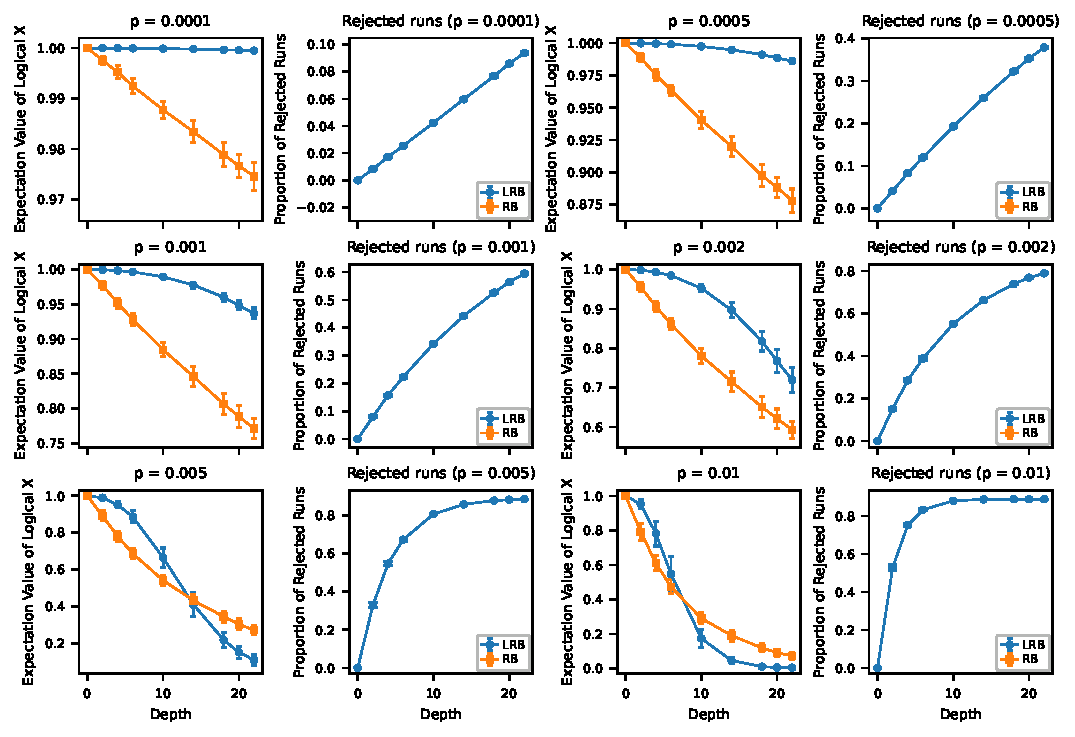
\includegraphics[width=0.78\textwidth]{figures/sdim140/sd6-1anc-const-0-nofit.pdf}
  \caption{Accepted logical signal $\langle \bar{X} \rangle$ of LRB-D (blue) and physical signal $\langle Z \rangle$ of physical RB at the same $p$ (orange) versus the depth $m$ (left panels) and fraction of rejected LRB-D shots (right panels) under terminal postselection and SD6, from the run of the one-ancilla layout. The points are joined by lines, not fits, and panels, labels, values of $p$ and error bars are as in \autoref{fig:const0_si1000_1anc}.}
  \label{fig:const0_sd6_1anc}
\end{figure*}

\begin{figure*}[tp]
  \centering
  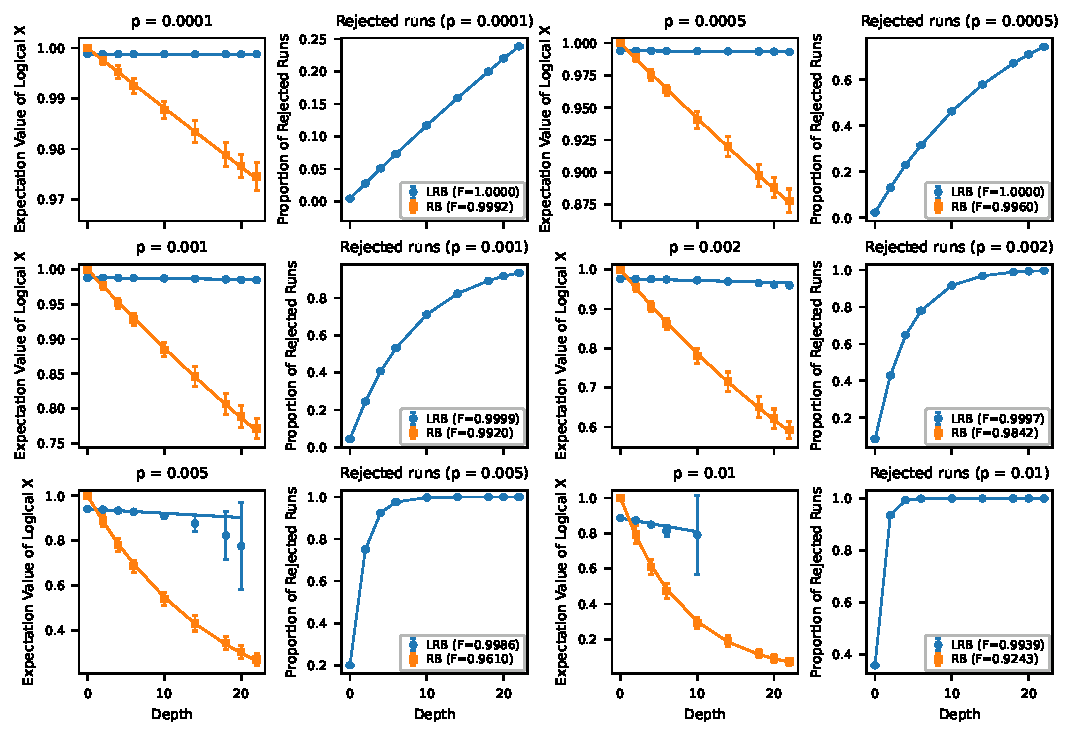
\includegraphics[width=0.78\textwidth]{figures/sdim140/sd6-1anc-unif-1-fit.pdf}
  \caption{Accepted logical signal $\langle \bar{X} \rangle$ of LRB-D (blue) and physical signal $\langle Z \rangle$ of physical RB at the same $p$ (orange) versus the depth $m$ (left panels), with the fits $F(m) = A f^m$ (lines), and fraction of rejected LRB-D shots (right panels), for uniform-interval postselection with interval $k = 1$ under SD6 in the one-ancilla layout. Panels, labels, values of $p$, legends, error bars and missing points are as in \autoref{fig:unif1_si1000_1anc}.}
  \label{fig:unif1_sd6_1anc}
\end{figure*}

\begin{figure*}[tp]
  \centering
  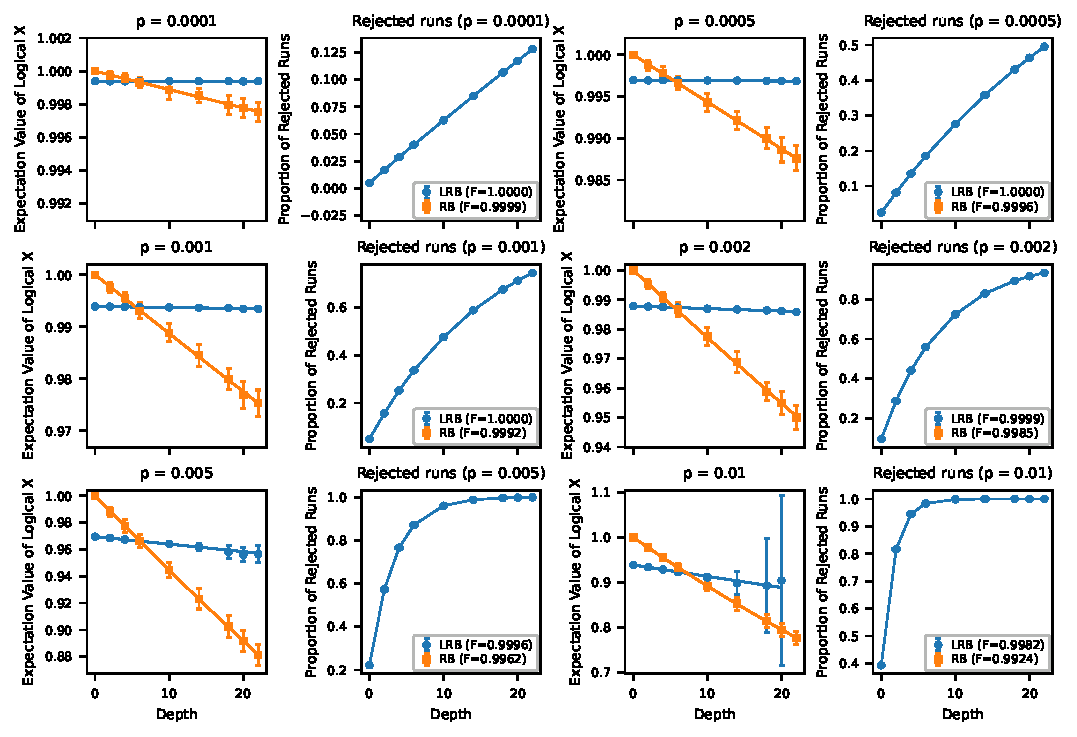
\includegraphics[width=0.78\textwidth]{figures/sdim140/si1000-1anc-unif-2-fit.pdf}
  \caption{Accepted logical signal $\langle \bar{X} \rangle$ of LRB-D (blue) and physical signal $\langle Z \rangle$ of physical RB at the same $p$ (orange) versus the depth $m$ (left panels), with the fits $F(m) = A f^m$ (lines), and fraction of rejected LRB-D shots (right panels), for uniform-interval postselection with interval $k = 2$ under SI1000 in the one-ancilla layout. Panels, labels, values of $p$, legends, error bars and missing points are as in \autoref{fig:unif1_si1000_1anc}.}
  \label{fig:unif2_si1000_1anc}
\end{figure*}

\begin{figure*}[tp]
  \centering
  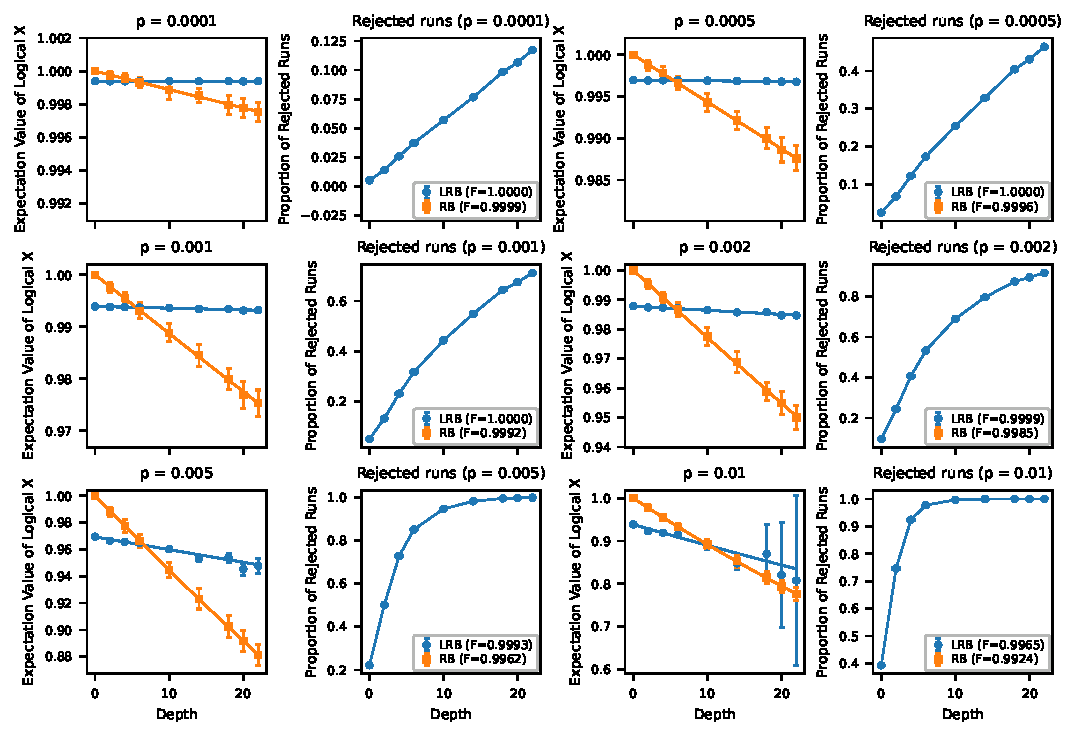
\includegraphics[width=0.78\textwidth]{figures/sdim140/si1000-1anc-unif-3-fit.pdf}
  \caption{Accepted logical signal $\langle \bar{X} \rangle$ of LRB-D (blue) and physical signal $\langle Z \rangle$ of physical RB at the same $p$ (orange) versus the depth $m$ (left panels), with the fits $F(m) = A f^m$ (lines), and fraction of rejected LRB-D shots (right panels), for uniform-interval postselection with interval $k = 3$ under SI1000 in the one-ancilla layout. Panels, labels, values of $p$, legends, error bars and missing points are as in \autoref{fig:unif1_si1000_1anc}.}
  \label{fig:unif3_si1000_1anc}
\end{figure*}

\begin{figure*}[tp]
  \centering
  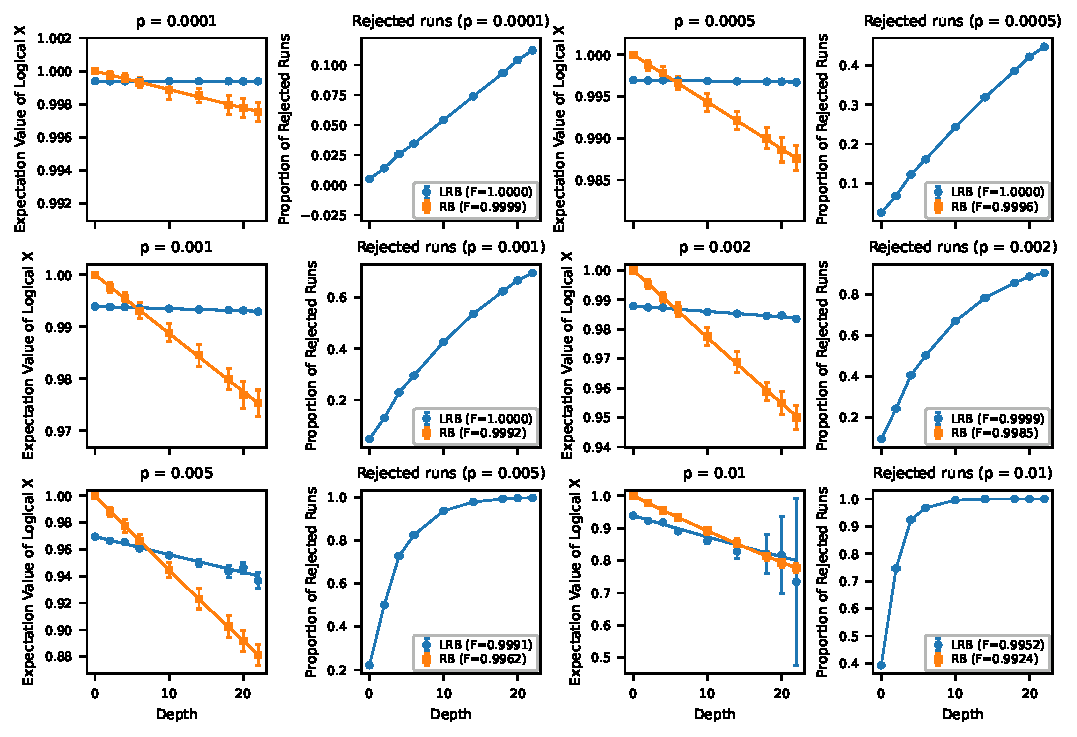
\includegraphics[width=0.78\textwidth]{figures/sdim140/si1000-1anc-unif-4-fit.pdf}
  \caption{Accepted logical signal $\langle \bar{X} \rangle$ of LRB-D (blue) and physical signal $\langle Z \rangle$ of physical RB at the same $p$ (orange) versus the depth $m$ (left panels), with the fits $F(m) = A f^m$ (lines), and fraction of rejected LRB-D shots (right panels), for uniform-interval postselection with interval $k = 4$ under SI1000 in the one-ancilla layout. Panels, labels, values of $p$, legends, error bars and missing points are as in \autoref{fig:unif1_si1000_1anc}.}
  \label{fig:unif4_si1000_1anc}
\end{figure*}

\begin{figure*}[tp]
  \centering
  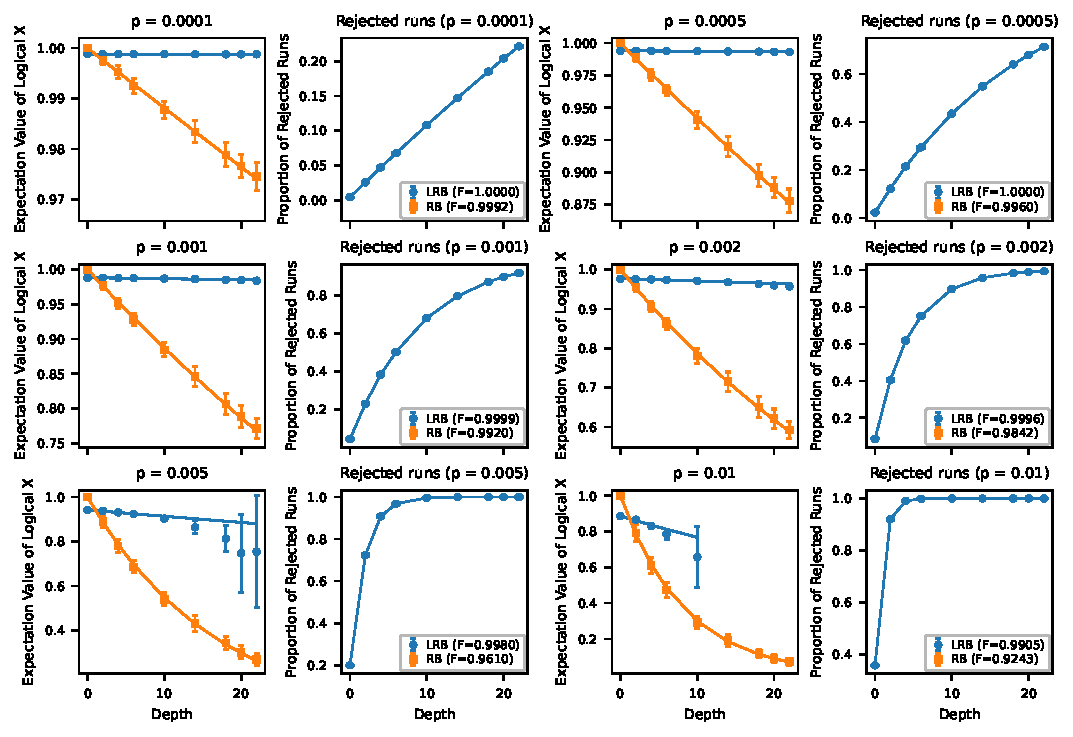
\includegraphics[width=0.78\textwidth]{figures/sdim140/sd6-1anc-unif-2-fit.pdf}
  \caption{Accepted logical signal $\langle \bar{X} \rangle$ of LRB-D (blue) and physical signal $\langle Z \rangle$ of physical RB at the same $p$ (orange) versus the depth $m$ (left panels), with the fits $F(m) = A f^m$ (lines), and fraction of rejected LRB-D shots (right panels), for uniform-interval postselection with interval $k = 2$ under SD6 in the one-ancilla layout. Panels, labels, values of $p$, legends, error bars and missing points are as in \autoref{fig:unif1_si1000_1anc}.}
  \label{fig:unif2_sd6_1anc}
\end{figure*}

\begin{figure*}[tp]
  \centering
  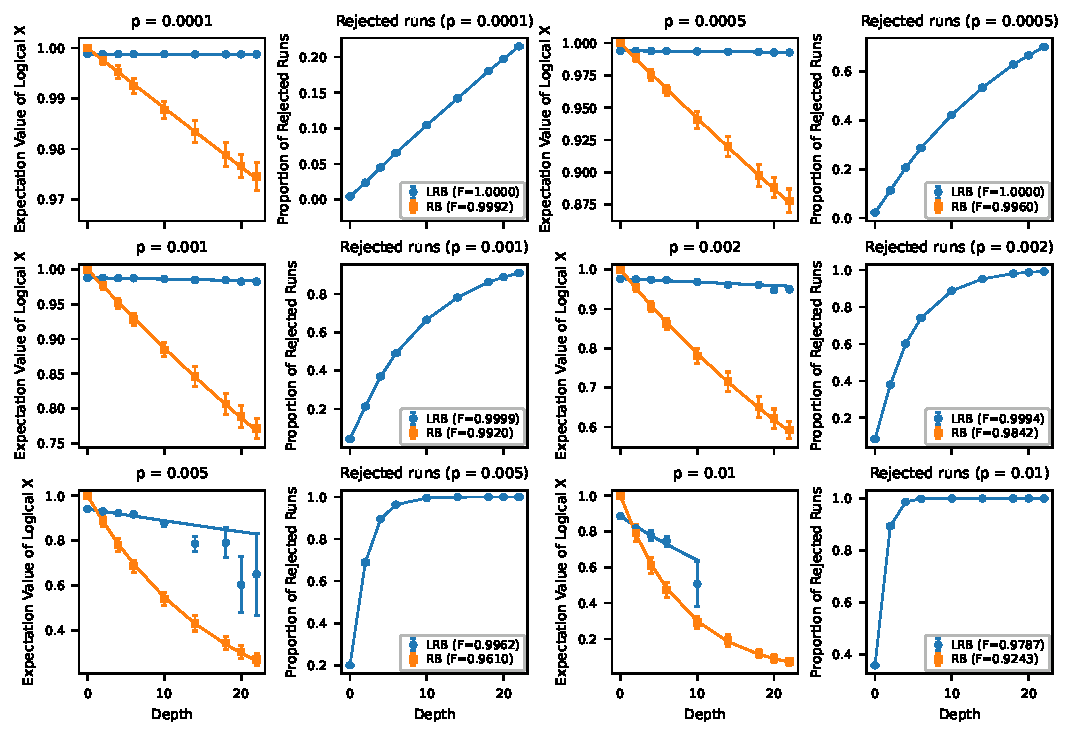
\includegraphics[width=0.78\textwidth]{figures/sdim140/sd6-1anc-unif-3-fit.pdf}
  \caption{Accepted logical signal $\langle \bar{X} \rangle$ of LRB-D (blue) and physical signal $\langle Z \rangle$ of physical RB at the same $p$ (orange) versus the depth $m$ (left panels), with the fits $F(m) = A f^m$ (lines), and fraction of rejected LRB-D shots (right panels), for uniform-interval postselection with interval $k = 3$ under SD6 in the one-ancilla layout. Panels, labels, values of $p$, legends, error bars and missing points are as in \autoref{fig:unif1_si1000_1anc}.}
  \label{fig:unif3_sd6_1anc}
\end{figure*}

\begin{figure*}[tp]
  \centering
  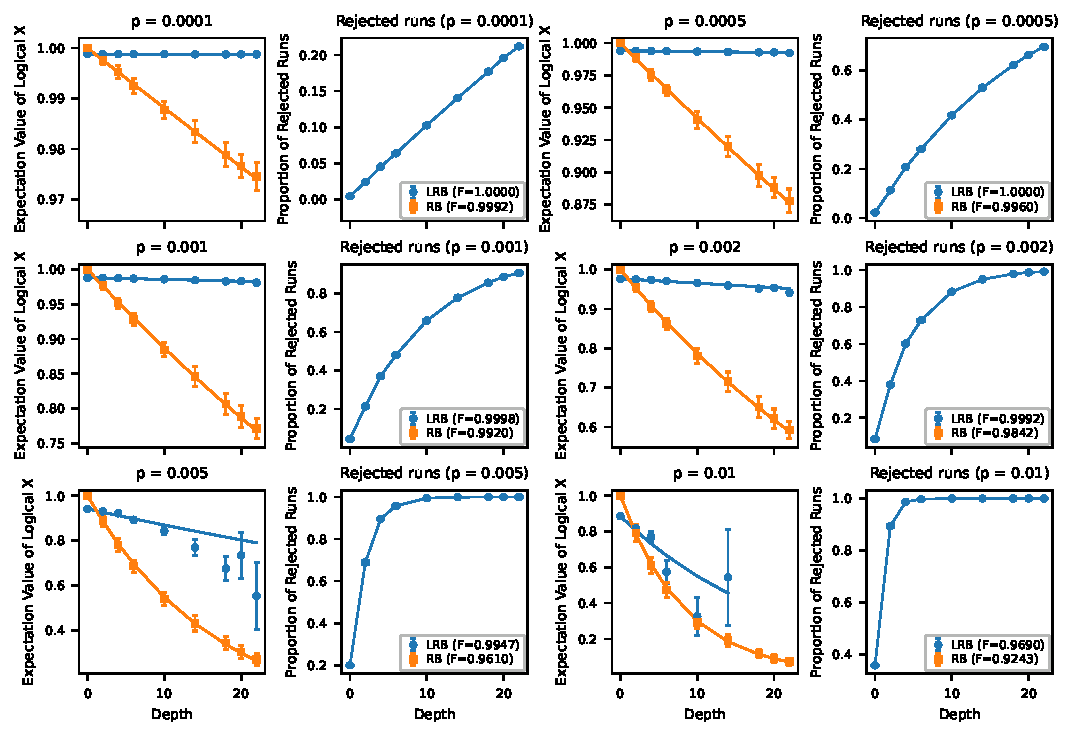
\includegraphics[width=0.78\textwidth]{figures/sdim140/sd6-1anc-unif-4-fit.pdf}
  \caption{Accepted logical signal $\langle \bar{X} \rangle$ of LRB-D (blue) and physical signal $\langle Z \rangle$ of physical RB at the same $p$ (orange) versus the depth $m$ (left panels), with the fits $F(m) = A f^m$ (lines), and fraction of rejected LRB-D shots (right panels), for uniform-interval postselection with interval $k = 4$ under SD6 in the one-ancilla layout. Panels, labels, values of $p$, legends, error bars and missing points are as in \autoref{fig:unif1_si1000_1anc}.}
  \label{fig:unif4_sd6_1anc}
\end{figure*}

\begin{figure*}[tp]
  \centering
  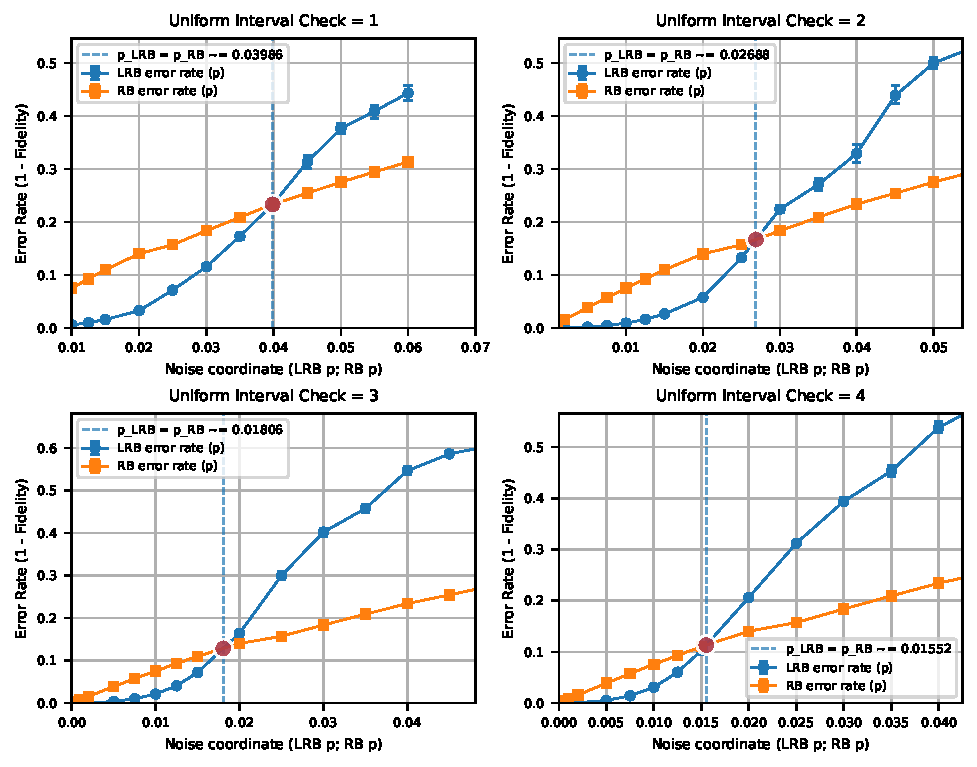
\includegraphics[width=0.75\textwidth]{figures/sdim140/sd6-1anc-threshold-grid.pdf}
  \caption{Fitted error rates per unit of depth of LRB-D (blue) and of the baseline, physical RB (orange), versus the two-qutrit gate error probability $p$ under SD6 in the one-ancilla layout, for the intervals $k = 1$ to $4$, with central 68\% intervals of the parametric bootstrap; intervals that are not visible are smaller than the markers. Each panel shows a window around $p^\star(k)$ of the grid that merges the two runs: points at $p < 0.025$ come from the production run and points at $p \ge 0.025$ from the high-$p$ extension run. Panel titles, axis labels, legends, the vertical line and the large marker are as in \autoref{fig:threshold_grid_si1000_1anc}.}
  \label{fig:threshold_grid_sd6_1anc}
\end{figure*}

\subsection{Two-Ancilla Layout}

\begin{figure*}[tp]
  \centering
  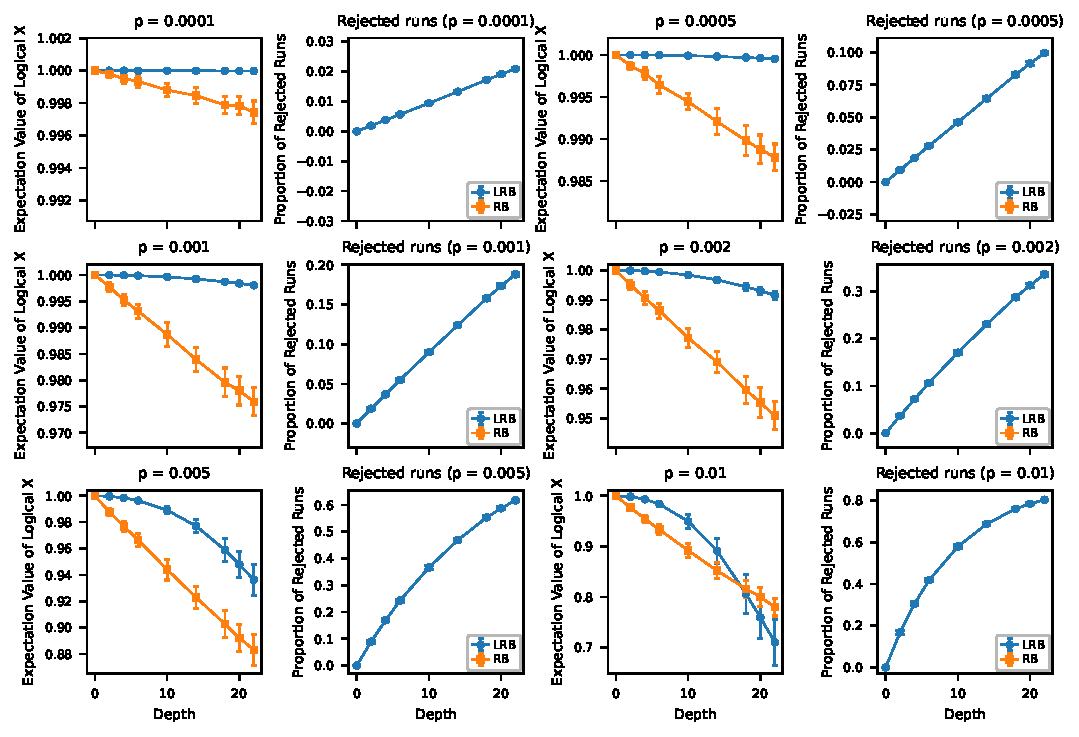
\includegraphics[width=0.78\textwidth]{figures/sdim140/si1000-conv-const-0-nofit.pdf}
  \caption{Accepted logical signal $\langle \bar{X} \rangle$ of LRB-D (blue) and physical signal $\langle Z \rangle$ of physical RB at the same $p$ (orange) versus the depth $m$ (left panels) and fraction of rejected LRB-D shots (right panels) under terminal postselection and SI1000, from the run of the two-ancilla layout. The points are joined by lines, not fits, and panels, labels, values of $p$ and error bars are as in \autoref{fig:const0_si1000_1anc}. The circuits are built as those of \autoref{fig:const0_si1000_1anc}, from 30 newly drawn sequences.}
  \label{fig:const0_si1000_2anc}
\end{figure*}

\begin{figure*}[tp]
  \centering
  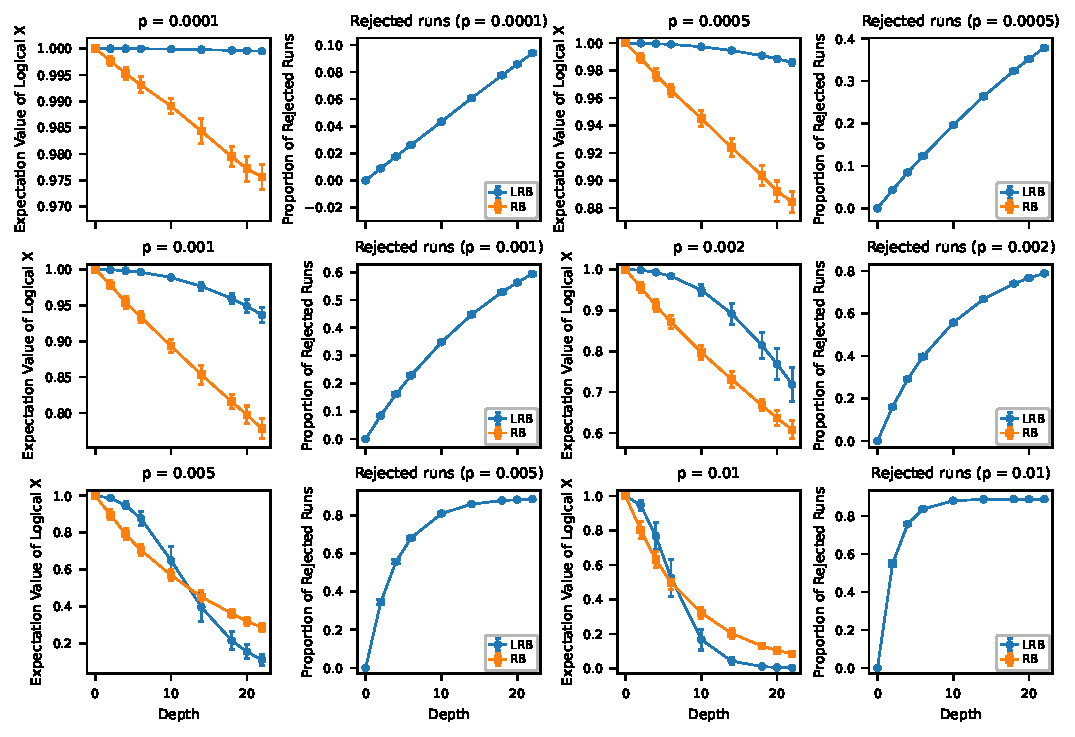
\includegraphics[width=0.78\textwidth]{figures/sdim140/sd6-conv-const-0-nofit.pdf}
  \caption{Accepted logical signal $\langle \bar{X} \rangle$ of LRB-D (blue) and physical signal $\langle Z \rangle$ of physical RB at the same $p$ (orange) versus the depth $m$ (left panels) and fraction of rejected LRB-D shots (right panels) under terminal postselection and SD6, from the run of the two-ancilla layout. The points are joined by lines, not fits, and panels, labels, values of $p$ and error bars are as in \autoref{fig:const0_si1000_1anc}. The circuits are built as those of \autoref{fig:const0_si1000_1anc}, from 30 newly drawn sequences.}
  \label{fig:const0_sd6_2anc}
\end{figure*}

\begin{figure*}[tp]
  \centering
  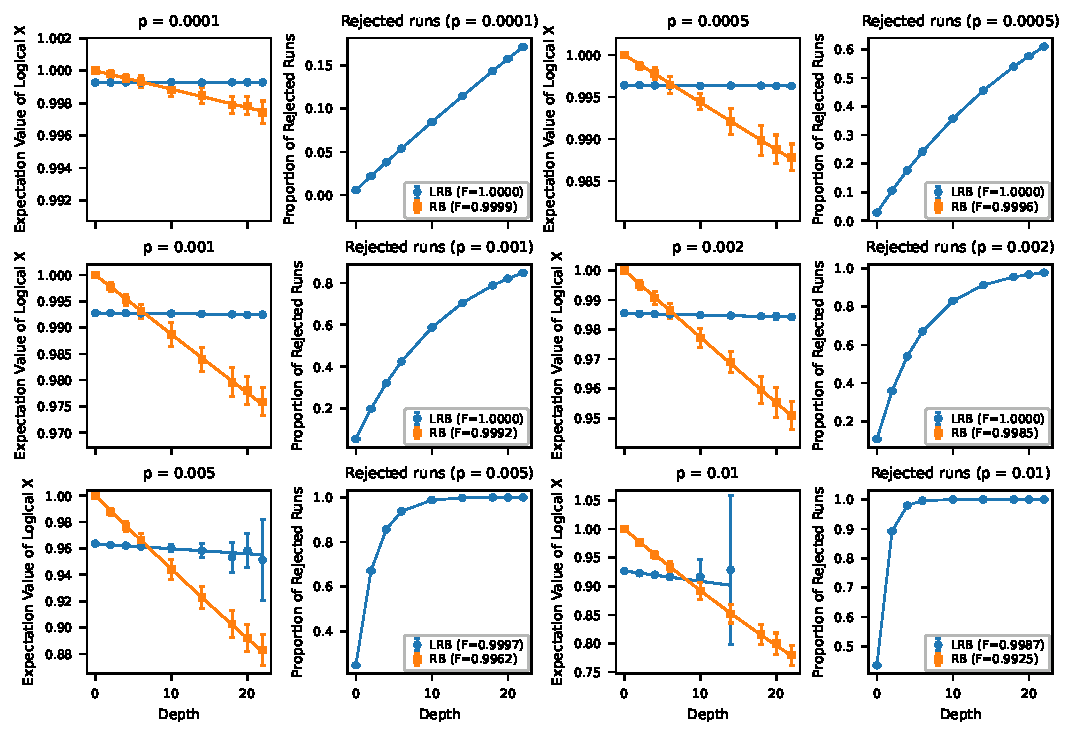
\includegraphics[width=0.78\textwidth]{figures/sdim140/si1000-conv-unif-1-fit.pdf}
  \caption{Accepted logical signal $\langle \bar{X} \rangle$ of LRB-D (blue) and physical signal $\langle Z \rangle$ of physical RB at the same $p$ (orange) versus the depth $m$ (left panels), with the fits $F(m) = A f^m$ (lines), and fraction of rejected LRB-D shots (right panels), for uniform-interval postselection with interval $k = 1$ under SI1000 in the two-ancilla layout. Panels, labels, values of $p$, legends, error bars and missing points are as in \autoref{fig:unif1_si1000_1anc}.}
  \label{fig:unif1_si1000_2anc}
\end{figure*}

\begin{figure*}[tp]
  \centering
  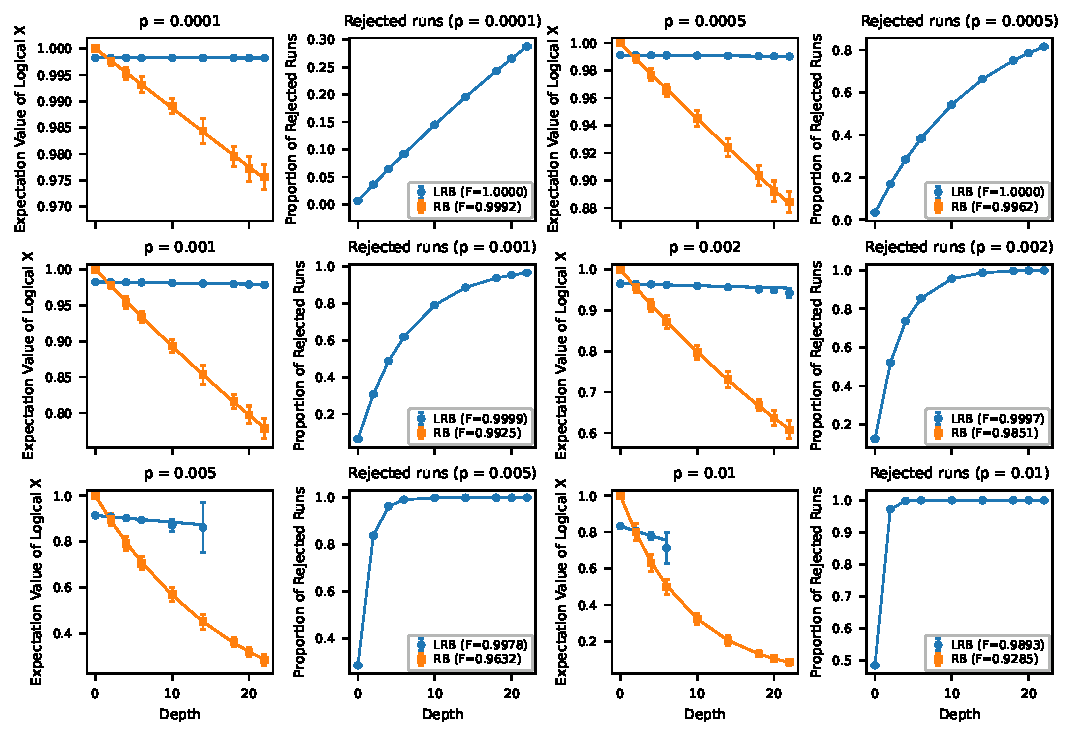
\includegraphics[width=0.78\textwidth]{figures/sdim140/sd6-conv-unif-1-fit.pdf}
  \caption{Accepted logical signal $\langle \bar{X} \rangle$ of LRB-D (blue) and physical signal $\langle Z \rangle$ of physical RB at the same $p$ (orange) versus the depth $m$ (left panels), with the fits $F(m) = A f^m$ (lines), and fraction of rejected LRB-D shots (right panels), for uniform-interval postselection with interval $k = 1$ under SD6 in the two-ancilla layout. Panels, labels, values of $p$, legends, error bars and missing points are as in \autoref{fig:unif1_si1000_1anc}.}
  \label{fig:unif1_sd6_2anc}
\end{figure*}

\begin{figure*}[tp]
  \centering
  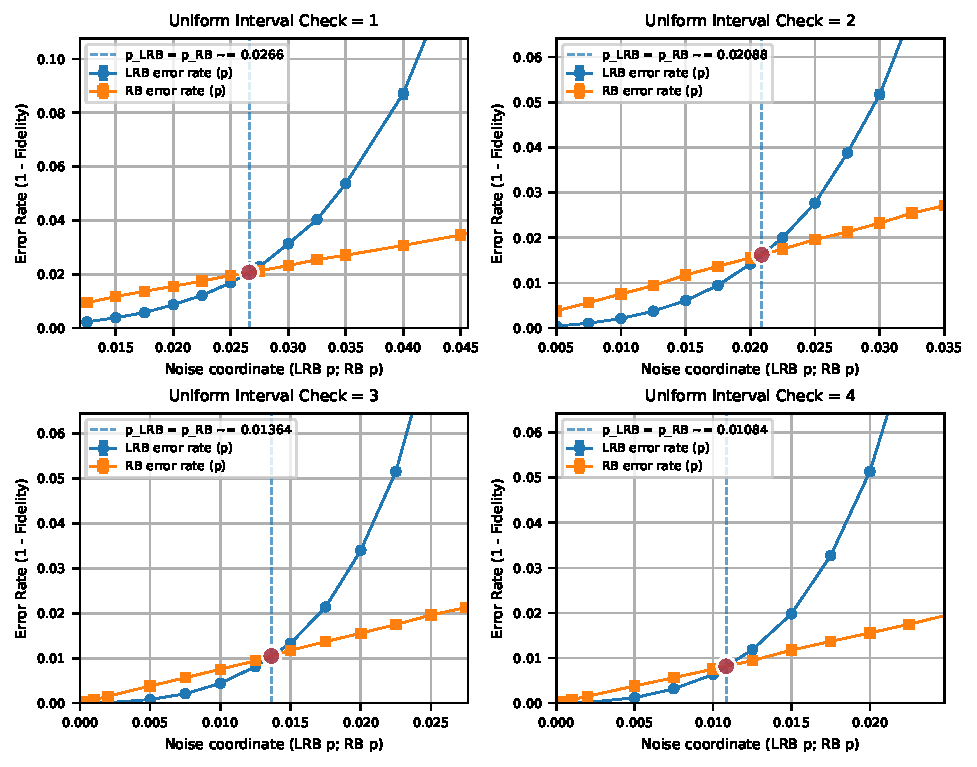
\includegraphics[width=0.85\textwidth]{figures/sdim140/si1000-conv-threshold-grid.pdf}
  \caption{Fitted error rates per unit of depth of LRB-D (blue) and of the baseline, physical RB (orange), versus the two-qutrit gate error probability $p$ under SI1000 in the two-ancilla layout, for the intervals $k = 1$ to $4$, with central 68\% intervals of the parametric bootstrap; intervals that are not visible are smaller than the markers. Each panel shows a window around $p^\star(k)$ of the grid that merges the two runs: points at $p < 0.015$ come from the production run and points at $p \ge 0.015$ from the high-$p$ extension run. Panel titles, axis labels, legends, the vertical line and the large marker are as in \autoref{fig:threshold_grid_si1000_1anc}.}
  \label{fig:threshold_grid_si1000_2anc}
\end{figure*}

\begin{figure*}[tp]
  \centering
  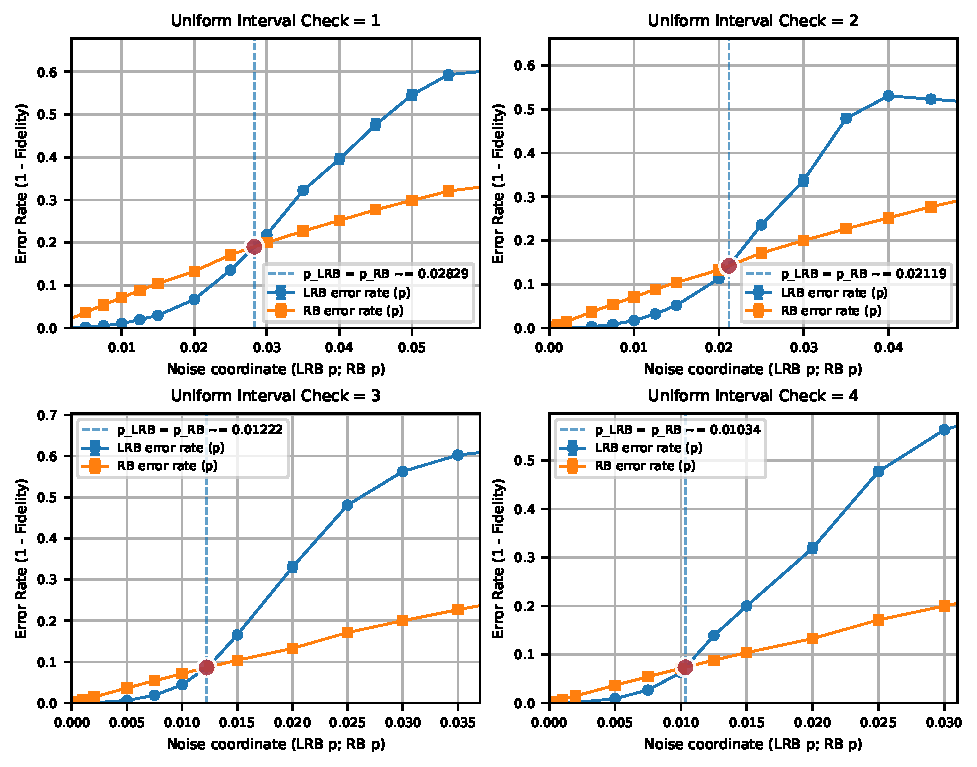
\includegraphics[width=0.80\textwidth]{figures/sdim140/sd6-conv-threshold-grid.pdf}
  \caption{Fitted error rates per unit of depth of LRB-D (blue) and of the baseline, physical RB (orange), versus the two-qutrit gate error probability $p$ under SD6 in the two-ancilla layout, for the intervals $k = 1$ to $4$, with central 68\% intervals of the parametric bootstrap; intervals that are not visible are smaller than the markers. Each panel shows a window around $p^\star(k)$ of the grid that merges the two runs: points at $p < 0.025$ come from the production run and points at $p \ge 0.025$ from the high-$p$ extension run. Panel titles, axis labels, legends, the vertical line and the large marker are as in \autoref{fig:threshold_grid_si1000_1anc}. In the $k = 2$ panel the LRB-D error rate falls from $0.531$ at $p = 0.04$ to $0.523$ at $p = 0.045$, between two fits over three depths each; the fall lies above $p^\star(2)$ and is too small to cut the grid of the search (\appref{app:campaign-search}).}
  \label{fig:threshold_grid_sd6_2anc}
\end{figure*}
 % D (track sim)

% Appendix E (track hw). Former Appendix B (review of representation theory, coauthor text, lightly
% edited) followed by the former main-text Sec. 3.2.6 (sub:irreps), rewritten, with the multiplicity
% computation that the paper lacked. Changes of content: jpw-review/hw/content-changes.md, part H.
\section{Representation Theory of the Twirled Channel}\label{sec:rep-theory}

\autoref{sub:fit_model} states that the Clifford twirl of the noise has two eigenvalues for a physical qutrit and up to $2542$ for the encoded qutrit. This appendix derives these numbers. It first reviews the results on representations of finite groups that the derivation uses, following~\cite{sagan2001symmetric}, and then applies them to the logical Clifford group of the $[[5,1,2]]_3$ code.

\subsection{Group Modules and Irreducible Representations}\label{app:rep-modules}

Let $G$ denote a finite group with identity element $e$.

A $G$-module is a finite dimensional vector space $V$ equipped with a group action $\cdot : G \times V \to V$ satisfying 
\begin{enumerate}
    \item \textbf{(Identity)} For all vectors $\ket{v} \in V$, the equality $e \cdot \ket{v} = \ket{v}$ is satisfied.
    \item \textbf{(Linearity)} For all linear combinations $\alpha \ket{v} + \beta \ket{w}$ and all group elements $g \in G$, the equality $g \cdot (\alpha \ket{v}+\beta\ket{w}) = \alpha (g\cdot \ket{v}) + \beta (g \cdot \ket{w})$ is satisfied.
    \item \textbf{(Compatibility)} For all group elements $g,h \in G$ and vectors $\ket{v} \in V$, the equality $(gh) \cdot \ket{v} = g\cdot (h \cdot \ket{v})$ is satisfied.
\end{enumerate}
The linearity axiom implies the existence of a map $\pi: G \to \mathrm{End}(V)$ mapping the group element $g$ to the linear endomorphism $\ket{v} \mapsto g\cdot \ket{v}$. 
The identity and compatibility axioms imply that $\pi$ is actually a group homomorphism. 

\begin{lemma}
    We call a group homomorphism $\pi : G \to \mathrm{End}(V)$ a representation of $G$. If $\pi: G \to \mathrm{End}(V)$ is a representation, then $V$ is a $G$-module under 
    \begin{align}
        g \cdot \ket{v} = \pi(g)\ket{v}.
    \end{align}
    Moreover, if $V$ is a $G$-module, then the map $\pi(g)(\ket{v}) = g\cdot \ket{v}$ is a representation of $G$.
\end{lemma}
We therefore use the terms representation of $G$ and $G$-module interchangeably.
As with all linear maps, representations are typically described by how each element of $G$ acts on each basis vector of $V$.
% Alternatively, one can describe a representation by first describing how the group $G$ acts on some set $X$ and then extending the action to the free vector space $\mathbb{C}[X]$ by linearity.

A representation can sometimes be reduced to a direct sum of smaller representations,
\begin{align}
    \pi(g) = \pi_0(g) \oplus \pi_1(g) \oplus \dots \oplus \pi_r(g) ,
\end{align}
with each $\pi_i$ a representation.
In this case, we write $\pi = \pi_0 \oplus \dots \oplus \pi_r$.
This corresponds to a decomposition of $G$-modules $V = V_0 \oplus \dots \oplus V_r$ where each $V_i$ is a $G$-module.
If no such decomposition exists, then we call the representation (or $G$-module) irreducible.
We abbreviate irreducible representation as irrep.

\begin{theorem}[Maschke's Theorem \cite{sagan2001symmetric} Theorem 1.5.3] \label{thm:maschkes-theorem}
    Every representation $\pi : G \to \mathrm{End}(V)$ decomposes into a direct sum
    \begin{align}
        \pi \cong m_0 \pi_0 \oplus m_1 \pi_1 \oplus \dots \oplus m_r \pi_r
    \end{align}
    where the $\pi_i$ are distinct irreducible representations of $G$ and $m_i \pi_i$ denotes the direct sum of $m_i$ copies of $\pi_i$. The integer $m_i$ is the multiplicity of $\pi_i$ in $\pi$.

    Similarly, if $V$ is a finite dimensional $G$-module, then 
    \begin{align}
        V = m_0 V_0 \oplus \dots \oplus m_r V_r
    \end{align}
    where the $V_i$ are distinct irreducible $G$-modules.
\end{theorem}
Maschke's theorem requires that the characteristic of the underlying field does not divide $|G|$, which holds over $\mathbb{C}$.
Its proof averages over the group, so an analog holds for compact Lie groups.
The form of Schur's lemma used below requires in addition an algebraically closed field such as $\mathbb{C}$.

\subsubsection{Schur's Lemma}

Suppose that $V$ is a $G$-module. 
We let $\mathrm{End}_G(V)$ denote all of the elements $T \in \mathrm{End}(V)$ such that for all $g \in G$
\begin{align}
    T \pi(g) = \pi(g)T.
\end{align}
Such elements $T$ are said to be invariant under the action of $G$, or $G$-linear.

\begin{lemma}[Schur's Lemma \cite{sagan2001symmetric} Theorem 1.6.5]\label{lem:schurs-lemma}
    Let $V$ and $W$ be $G$-modules and let $\pi_V$ and $\pi_W$ be the associated representations.
    We define $\mathrm{Hom}_G(V, W)$ by $T \in \mathrm{Hom}_G(V, W)$ if for all $g \in G$
    \begin{align}
        T \pi_V(g) = \pi_W(g) T.
    \end{align}
    If $V$ and $W$ are irreducible, then exactly one of the following holds.
    \begin{enumerate}
        \item The $G$-modules $V$ and $W$ are not isomorphic and $\mathrm{Hom}_G(V,W) = 0$.
        \item The $G$-modules $V$ and $W$ are isomorphic and $\mathrm{Hom}_G(V,W) \cong \mathbb{C}$ in the sense that $\mathrm{End}_G(V) = \{ \lambda I_V \mid \lambda \in \mathbb{C} \}$.
    \end{enumerate}
\end{lemma}

\begin{cor}[\cite{sagan2001symmetric} Theorem 1.7.9]\label{cor:schur-decomposition}
    Let $V$ be a $G$-module such that
    \begin{align}
        V = m_0 V_0 \oplus \dots \oplus m_r V_r
    \end{align}
    with the $V_i$ distinct irreducible modules.
    Let $d_i$ be the dimension of $V_i$.
    Then the following hold.
    \begin{enumerate}
        \item The dimension of $V$ is given by $\mathrm{dim}(V) = m_0 d_0 + \dots + m_r d_r$.
        \item \label{item:artin-wedderburn} The endomorphism algebra of $V$ is isomorphic to the direct sum
        \begin{align}
            \mathrm{End}_G(V) \cong \bigoplus_{i = 0}^r \mathrm{End}(\mathbb{C}^{m_i}).
        \end{align}
        \item The endomorphism algebra $\mathrm{End}_G(V)$ has dimension $m_0^2 + m_1^2 + \dots + m_r^2$.
    \end{enumerate}
\end{cor}

\begin{proof}
    We prove only item~\ref{item:artin-wedderburn}, the one used below.
    From the decomposition of $V$, we get the equality
    \begin{align}
        \mathrm{End}_G(V) \cong \bigoplus_{i,j = 0}^r \mathrm{Hom}_G(m_iV_i,m_jV_j).
    \end{align}
    The elements of $\mathrm{Hom}_G(m_i V_i, m_j V_j)$ can be thought of as $m_i \times m_j$ matrices whose entries are in $\mathrm{Hom}_G(V_i, V_j)$. 
    However, if $i \neq j$, then by Schur's lemma we know that $\mathrm{Hom}_G(V_i, V_j)$ only contains the zero map. 
    Thus, all of the terms in the direct sum for $i \neq j$ are zero and can be ignored. 
    When $i = j$, the elements of $\mathrm{Hom}_G(V_i,V_i) = \mathrm{End}_G(V_i)$ are all multiples of the identity map. 
    So, the elements $g_i \in \mathrm{End}_G(m_iV_i)$ can be written in the form
    \begin{align}
        g_i = M_i \otimes I_{V_i},
    \end{align}
    where $M_i \in \mathrm{End}(\mathbb{C}^{m_i})$ is an $m_i \times m_i$ matrix with complex entries. 
    % Moreover, any such matrix $M_i$ defines an element $g_i = M_i \otimes I_{V_i} \in \mathrm{End}_G(m_i V_i)$.
    A routine argument shows $\mathrm{End}_G(m_iV_i)$ is isomorphic to the matrix algebra $\mathrm{End}(\mathbb{C}^{m_i})$ under the map $g_i \mapsto M_i$.
    Finally, we conclude that $\mathrm{End}_G(V) \cong \bigoplus_{i = 0}^r \mathrm{End}_G(m_i V_i)$ and hence
    \begin{align}
        \mathrm{End}_G(V) \cong \bigoplus_{i=0}^r \mathrm{End}(\mathbb{C}^{m_i}).
    \end{align}
\end{proof}

The property of $\mathrm{End}_G(V)$ that we use is the following: if $T \in \mathrm{End}_G(V)$ and $\ket{v} \in m_i V_i$ is supported entirely in copies of the module $V_i$, then $T\ket{v} \in m_i V_i$ is also supported entirely in copies of $V_i$.
The next lemma guarantees that a twirled map is of this kind.

\begin{lemma}[Twirling] \label{lem:twirling}
    Suppose $V$ is a finite-dimensional $G$-module with associated representation $\pi$, for $G$ finite. Given any $T \in \mathrm{End}(V)$, which need not be $G$-linear, the twirled map
    \begin{align}
        T_G = \frac{1}{|G|} \sum_{g \in G} \pi(g)^{-1} T \pi(g)
    \end{align}
    is an element of $\mathrm{End}_G(V)$.
\end{lemma}

\begin{proof}
    Fix $g \in G$. Conjugating $T_G$ by $\pi(g)$ yields 
    \begin{align}
        \pi(g)^{-1} T_G \pi(g) &= \frac{1}{|G|} \sum_{h \in G} \pi(g)^{-1} \pi(h)^{-1} T \pi(h) \pi(g) \nonumber \\
        &= \frac{1}{|G|} \sum_{h \in G} \pi(hg)^{-1} T \pi(hg).
    \end{align}
    Since the right coset $Gg$ is equal to $G$, we can reindex the sum to obtain 
    \begin{align}
        \pi(g)^{-1} T_G \pi(g) &= \frac{1}{|G|} \sum_{h \in G} \pi(hg)^{-1} T \pi(hg) \nonumber \\
        &= \frac{1}{|G|} \sum_{h \in G} \pi(h)^{-1} T \pi(h) = T_G.
    \end{align}
    We conclude that $\pi(g)^{-1} T_G \pi(g) = T_G$ and hence $T_G \pi(g) = \pi(g) T_G$.
\end{proof}

\subsection{Character Theory}\label{app:rep-characters}

By item~\ref{item:artin-wedderburn} of Corollary~\ref{cor:schur-decomposition} and Lemma~\ref{lem:twirling}, the structure of a twirled map is fixed by the multiplicity of each irrep in the representation.
Character theory computes these multiplicities once the irreps are known.

\subsubsection{Characters and Conjugacy Classes}

If $\pi : G \to \mathrm{End}(V)$ is a representation, then the character $\chi_\pi : G \to \mathbb{C}$ of $\pi$ is defined by 
\begin{align}
    \chi_\pi(g) = \Tr \pi(g).
\end{align}
By the cyclic property of the trace, characters satisfy the property $\chi_\pi(h g h^{-1}) = \chi_\pi(g)$.
Characters are therefore constant on the conjugacy classes.
Such a function is called a class function.
The space of class functions has dimension equal to the number of conjugacy classes of $G$, and it carries the inner product

\begin{align}
    \langle \chi, \tau \rangle = \frac{1}{|G|} \sum_{g \in G} \chi(g)^* \tau(g).
\end{align}

\begin{lemma}[Character Orthogonality \cite{sagan2001symmetric} Theorem 1.9.3] \label{lem:character-orthogonality}
    If $\pi_1$ and $\pi_2$ are irreducible representations of the finite group $G$, then 
    \begin{align}
        \langle \chi_{\pi_1}, \chi_{\pi_2}\rangle = \begin{cases}
            1 & \pi_1 \cong \pi_2, \\
            0 & \text{otherwise}.
        \end{cases}
    \end{align}
\end{lemma}

\begin{cor}[\cite{sagan2001symmetric} Corollary 1.9.4] \label{cor:character-relations}
    Let $\pi : G \to \mathrm{End}(V)$ be a representation and $\pi = m_0 \pi_0 \oplus \dots \oplus m_r \pi_r$ be the decomposition of the representation $\pi$ into irreps. The following hold.
    \begin{enumerate}
        \item The character $\chi_{\pi}$ can be written as $\chi_{\pi} = m_0 \chi_{\pi_0} + m_1 \chi_{\pi_1} + \dots + m_r \chi_{\pi_r}$.
        \item \label{item:irrep-mult-test} The inner product $\langle \chi_{\pi}, \chi_{\pi_i}\rangle = m_i$ for all $0 \leq i \leq r$.
        \item The inner product $\langle \chi_{\pi}, \chi_{\pi} \rangle = m_0^2 + \dots + m_r^2$. In particular this is always an integer.
        \item The representation $\pi$ is irreducible if and only if $\langle \chi_{\pi}, \chi_{\pi} \rangle = 1$.
        \item If $\tau$ is another representation of $G$, then $\pi$ and $\tau$ are isomorphic if and only if $\chi_{\pi}(g) = \chi_{\tau}(g)$ for all $g \in G$.
    \end{enumerate}
\end{cor}

Lemma~\ref{lem:character-orthogonality} and Corollary~\ref{cor:character-relations} have two consequences that we use.
First, the irrep characters are orthonormal and thus linearly independent.
Together with the completeness of the irreducible characters, which span the space of class functions~\cite{sagan2001symmetric}, this shows that the irrep characters form a basis for that space and, in particular, that there are exactly as many irreps as there are conjugacy classes of $G$.
Second, item~\ref{item:irrep-mult-test} of Corollary~\ref{cor:character-relations} gives the multiplicity of an irrep in any representation of $G$ as an inner product of characters.

\subsection{The Logical Clifford Group of the \texorpdfstring{$[[5,1,2]]_3$}{[[5,1,2]]3} Code}
\label{sub:irreps}

% Former main-text Sec. 3.2.6 ("method - LRB-D.tex", lines 245-303 of the 438f6f16 mirror), rewritten. New here: the characters and the two inner products that give the multiplicities, and the table of all ten.
% All numbers of this subsection: paper-rework/scratch/lead/irreps_check.py (output in jpw-review/hw/checks/irreps_check.out): conjugation representation of the 216-element group generated by the physical Hbar and Sbar, built with sdim's gate matrices; Burnside character table of the logical action; multiplicities 301, 260, 260 (dimension 1), 560, 560, 520 (dimension 2), 820 (dimension 3), 2160, 2160, 2241 (dimension 8, the last being V_pauli); sum of m*d = 59049; the group with Xbar and Zbar has 1944 elements, m_triv = 40, m_pauli = 261; its nine-element kernel on the code space is generated by G_2 and G_4.
We now apply these results to the encoded qutrit. Let $\mathcal{H}$ be the $3^5$-dimensional Hilbert space of the five data qutrits and $\mathcal{S}$ the $3^{10}$-dimensional space of linear operators on $\mathcal{H}$, on which density operators live and noise channels act. Let $\bar{\mathcal{C}}_3$ be the group generated by the five-qutrit unitaries $\bar H$ and $\bar S$ of Eqs.~\eqref{eq:logical_H} and~\eqref{eq:logical_HS}, taken up to global phases. It has $216$ elements, and its action on the code space maps it one-to-one onto the single-qutrit Clifford group $\mathcal{C}_3$. Conjugation,
\begin{equation}
    \bar{\pi}(C)(\rho) = \bar{C} \rho\, \bar{C}^\dagger ,
\end{equation}
where $\bar C \in \bar{\mathcal{C}}_3$ is the unitary that implements $C \in \mathcal{C}_3$ on the logical qutrit, is therefore a representation of $\mathcal{C}_3$ on $\mathcal{S}$. The module of this representation is the operator space $\mathcal{S}$ and not $\mathcal{H}$.

% TODO(authors): cite the paper that lists the conjugacy classes of the single-qutrit Clifford group (was a red author note in the text; jpw-review/OPEN-QUESTIONS.md, item 7).
Up to global phases, $\mathcal{C}_3$ has $10$ conjugacy classes, of sizes $1$, $8$, $9$, $12$, $12$, $24$, $24$, $36$, $36$ and $54$, and hence $10$ irreps (\autoref{tab:irreps}). Two of them matter here. The first is the trivial irrep $V_{\mathrm{triv}}$. The second is the eight-dimensional irrep $V_{\mathrm{pauli}}$ in which $\mathcal{C}_3$ conjugates the eight traceless Pauli operators of one qutrit. The operators of one qutrit decompose as $V_{\mathrm{triv}} \oplus V_{\mathrm{pauli}}$, which is the origin of the two eigenvalues of Eq.~\eqref{eq:twirl_irrep}. By Theorem~\ref{thm:maschkes-theorem}, the operators of five qutrits decompose as
\begin{equation}
    \mathcal{S} \cong m_{\mathrm{triv}} V_{\mathrm{triv}} \oplus m_{\mathrm{pauli}} V_{\mathrm{pauli}} \oplus \bigoplus_{i = 2}^{9} m_i V_i ,
    \label{eq:irrep-decomposition}
\end{equation}
where $V_2, \dots, V_9$ are the other eight irreps.

The multiplicities follow from item~\ref{item:irrep-mult-test} of Corollary~\ref{cor:character-relations}. Conjugation by a unitary $U$ acts on the operator space as $U \otimes U^{*}$, whose trace is $\lvert \Tr U \rvert^2$, so the character of $\bar\pi$ is $\chi_{\bar\pi}(C) = \lvert \Tr \bar C \rvert^2$. In the same way the character of one-qutrit conjugation is $\lvert \Tr C \rvert^2$, with $C$ taken as a $3 \times 3$ unitary, and the character of $V_{\mathrm{pauli}}$ is $\chi_{\mathrm{pauli}}(C) = \lvert \Tr C \rvert^2 - 1$. The two multiplicities are therefore
\begin{equation}
  \begin{aligned}
    m_{\mathrm{triv}} &= \frac{1}{216} \sum_{C \in \mathcal{C}_3} \lvert \Tr \bar C \rvert^2 = 301 , \\
    m_{\mathrm{pauli}} &= \frac{1}{216} \sum_{C \in \mathcal{C}_3} \left( \lvert \Tr C \rvert^2 - 1 \right) \lvert \Tr \bar C \rvert^2 = 2241 ,
  \end{aligned}
  \label{eq:multiplicities}
\end{equation}
which we evaluated numerically from the $216$ five-qutrit unitaries. \autoref{tab:irreps} lists the multiplicities of all ten irreps, for which we computed the remaining characters from the multiplication table of the group. They satisfy $\sum_i m_i \dim V_i = 3^{10}$. For one physical qutrit, $m_{\mathrm{triv}} = m_{\mathrm{pauli}} = 1$ and all other multiplicities vanish.

\begin{table*}[tp]
  \centering
  \begin{tabular}{l|cccccccccc}
    \hline
    Irrep & $V_{\mathrm{triv}}$ & $V_2$ & $V_3$ & $V_4$ & $V_5$ & $V_6$ & $V_7$ & $V_8$ & $V_9$ & $V_{\mathrm{pauli}}$ \\
    \hline
    Dimension & 1 & 1 & 1 & 2 & 2 & 2 & 3 & 8 & 8 & 8 \\
    Multiplicity & 301 & 260 & 260 & 560 & 560 & 520 & 820 & 2160 & 2160 & 2241 \\
    \hline
  \end{tabular}
  \caption{The ten irreps of the single-qutrit Clifford group $\mathcal{C}_3$ and their multiplicities in the conjugation representation $\bar\pi$ of the group generated by $\bar H$ and $\bar S$ on the $3^{10}$-dimensional operator space of the five data qutrits.}
  \label{tab:irreps}
\end{table*}

The simulated gate set generates a larger group. It applies the logical Pauli operators as $\bar X = X_0 X_3$ and $\bar Z = Z_0 Z_2$ (Eq.~\eqref{eq:logicalPauli}), which differ from the elements of $\bar{\mathcal{C}}_3$ with the same logical action by the stabilizers $G_4$ and $G_2$. The group generated by $\bar H$, $\bar S$, $\bar X$ and $\bar Z$ thus consists of the products of the elements of $\bar{\mathcal{C}}_3$ with the nine products of powers of $G_2$ and $G_4$. It has $1944$ elements and acts on the code space as $\bar{\mathcal{C}}_3$ does. The same computation for this group gives $m_{\mathrm{triv}} = 40$ and $m_{\mathrm{pauli}} = 261$.

These multiplicities bound the number of eigenvalues that a decay can contain. Let $\mathrm{End}_{\mathcal{C}_3}(\mathcal{S})$ be the set of linear maps on $\mathcal{S}$ that commute with $\bar\pi$. By item~\ref{item:artin-wedderburn} of Corollary~\ref{cor:schur-decomposition} it is isomorphic, as an algebra, to a direct sum of matrix algebras,
\begin{align}
    \mathrm{End}_{\mathcal{C}_3}(\mathcal{S}) &\cong \mathrm{Mat}_{m_{\mathrm{triv}}}(\mathbb{C}) \otimes I_{V_{\mathrm{triv}}} \nonumber \\
    &\quad \oplus \mathrm{Mat}_{m_{\mathrm{pauli}}}(\mathbb{C})\otimes I_{V_{\mathrm{pauli}}} \nonumber \\
    &\quad \oplus \bigoplus_{i = 2}^9 \mathrm{Mat}_{m_i} (\mathbb{C}) \otimes I_{V_i} ,
\end{align}
so that such a map cannot take a vector of $m_i V_i$ to a vector with a component in $m_j V_j$ for $j \neq i$. The twirled error channel $\Lambda_{\mathrm{eff}}$ is a map of this kind by Lemma~\ref{lem:twirling}, and in a suitable basis it reads
\begin{equation}
    \Lambda_{\mathrm{eff}} = M_{\mathrm{triv}}\otimes I_{V_{\mathrm{triv}}} \oplus M_{\mathrm{pauli}} \otimes I_{V_{\mathrm{pauli}}} \oplus M ,
\end{equation}
where $M_{\mathrm{triv}}$ and $M_{\mathrm{pauli}}$ are square matrices of sizes $m_{\mathrm{triv}}$ and $m_{\mathrm{pauli}}$ and $M$ collects the other eight irreps. If $M_{\mathrm{triv}}$ and $M_{\mathrm{pauli}}$ are diagonalizable, a further change of basis gives
\begin{equation}
  \begin{aligned}
    \Lambda_{\mathrm{eff}} &= \Lambda_{\mathrm{triv}} \oplus \Lambda_{\mathrm{pauli}} \otimes I_{V_{\mathrm{pauli}}} \oplus M , \\
    \Lambda_{\mathrm{eff}}^{\,t} &= \Lambda_{\mathrm{triv}}^{\,t} \oplus \Lambda_{\mathrm{pauli}}^{\,t} \otimes I_{V_{\mathrm{pauli}}} \oplus M^{t} ,
  \end{aligned}
  \label{eq:twirl-logical}
\end{equation}
with $\Lambda_{\mathrm{triv}}$ and $\Lambda_{\mathrm{pauli}}$ the diagonal matrices of their eigenvalues and $t$ the number of applications of the channel.

The block $M$ does not act on a state of the code space. The operators supported on the code space transform under $\bar\pi$ as the operators of one qutrit, so a code state such as $\ket{\bar{+}}\bra{\bar{+}}$ decomposes as $\rho = \rho_{\mathrm{triv}} \oplus \rho_{\mathrm{pauli}} \oplus 0$ with $\rho_{\mathrm{triv}} \in m_{\mathrm{triv}} V_{\mathrm{triv}}$ and $\rho_{\mathrm{pauli}} \in m_{\mathrm{pauli}}V_{\mathrm{pauli}}$. By Eq.~\eqref{eq:twirl-logical} its evolution under repeated application of $\Lambda_{\mathrm{eff}}$ contains only the powers of the diagonal elements of $\Lambda_{\mathrm{triv}}$ and $\Lambda_{\mathrm{pauli}}$. There are $m_{\mathrm{triv}} + m_{\mathrm{pauli}} = 301 + 2241 = 2542$ of them for $\bar{\mathcal{C}}_3$, and $40 + 261 = 301$ for the group that the simulated gate set generates, against $1 + 1 = 2$ for a physical qutrit. If $M_{\mathrm{triv}}$ or $M_{\mathrm{pauli}}$ is not diagonalizable, its Jordan form takes the place of the diagonal matrix, and a Jordan block of size $s$ with eigenvalue $\lambda$ contributes the terms $\binom{t}{j}\lambda^{t-j}$ with $j < s$ in place of the single power $\lambda^t$.
 % E (track hw; parked text until M3)

% Appendix F (track hw). Former Appendix C of the 438f6f16 mirror, without the parts that restate
% Secs. 2.3, 2.5 and 2.7 (run list, definition of the check rounds and of the schedules, logical
% readout), without the statement "All circuits in this work use q = 3" and without the const-n
% schedules, for which the paper reports no result. Changes of content:
% jpw-review/hw/content-changes.md, part I.
\section{The \texttt{sdim} Simulator and Detector-Error-Model Sampling}
\label{sec:sdim-dem}

\autoref{sub:sim_framework} states that sampling the detector error model (DEM) of a circuit reproduces the joint distribution of its detectors and of its logical outcome without approximation. This appendix describes how \texttt{sdim}~1.4.0~\cite{sdim} builds and samples the model and why the sampling is exact. The formulas are written for qutrits. For the qubit code, $q = 2$ takes the place of $q = 3$.

\subsection{Qudit Stabilizer Simulation}
\label{app:sdim-simulator}

% from "sdim dem appendix.tex", lines 8-12 of the mirror
\texttt{sdim} is a tableau-based stabilizer simulator for qudits of prime dimension $q$. It generalizes the binary tableau formalism of~\cite{Aaronson2004} to arithmetic over $\mathbb{Z}_q$ and represents stabilizer generators as Pauli operators $\omega^c X^{\mathbf{a}} Z^{\mathbf{b}}$ with exponent vectors $\mathbf{a}, \mathbf{b} \in \mathbb{Z}_q^n$~\cite{Gottesman1999,Hostens2005}. Clifford gates act on the tableau by linear updates of these exponent vectors, and measurements follow the qudit analog of the stabilizer measurement rules. Each noise channel of \autoref{tab:circuit-noise} is an explicit operation in the circuit, with the probability of its location.

Rather than rerunning the tableau algorithm for every shot, \texttt{sdim} samples in the Pauli-frame picture. It simulates one noiseless reference shot with the tableau algorithm. For every further shot it propagates only a Pauli frame, one pair of exponents $(a_i, b_i)$ per qutrit, through the Clifford circuit. Noise operations update the frame at random, and each computational-basis measurement returns the reference outcome shifted by the $X$ exponent of the frame on the measured qutrit, modulo three. As in Stim~\cite{Gidney2021Stim}, the frame simulator draws a random $Z$ component of the frame at the start of the circuit and after every computational-basis measurement and reset, which accounts for measurement outcomes that are random in the reference shot. The stabilizer computation, whose cost is polynomial in the number of qutrits, is thus done once, and the work per shot is the propagation of the frame.

\subsection{Detectors and Logical Observables}
\label{app:sdim-detectors}

% from "sdim dem appendix.tex", lines 16-22 of the mirror
The detectors of \autoref{sub:sim_framework} are linear in the measurement records $m_i$ of a circuit, $D = \sum_i c_i m_i \bmod 3$ with integer coefficients $c_i$. A logical observable is an expression of the same kind on the logical readout. In our circuits it also takes a fixed value in the absence of noise, because the mirror inverse returns the initial state, and a deviation from this value is a logical error. This is the qudit form of the detector formalism of Stim~\cite{Gidney2021Stim}, with sums modulo three in place of sums modulo two and with coefficients $\pm 1$ for the stabilizer factors that enter with an inverse.

In an LRB-D circuit every ancilla readout of every check round is one detector with coefficient one, because each ancilla is reset before its round and reads zero in the absence of noise. A circuit of depth $m$ therefore has $4(m+1)$ detectors in either layout, $92$ at depth $22$, and its observable is the logical outcome of \autoref{sub:lrb_d}. The circuits of terminal postselection have the same observable and two detectors, the values of $G_3$ and $G_4$. The baseline circuits have no detector, and their observable is the final readout of the qutrit. The postselection acts on the sampled detector values and is not part of the circuit. Because all intervals $k$ share the shots, the estimates for different intervals at the same $p$, sequence and depth are statistically correlated.

\subsection{The Detector Error Model}
\label{app:sdim-model}

% from "sdim dem appendix.tex", lines 26-31 of the mirror
A DEM is a list of independent error mechanisms, each with a firing probability and its effect on every detector and observable. The construction rests on linearity. Write a Pauli fault on the $n \in \{1,2\}$ qutrits of one noise operation, up to a phase, as an exponent vector $e = (a_1, b_1, \dots, a_n, b_n) \in \mathbb{Z}_3^{2n}$. The fault propagates through the rest of the Clifford circuit to a Pauli frame whose exponents depend linearly on $e$, and detectors and observables are linear in the measurement records. The fault therefore shifts the vector of all detector and observable values by
\begin{equation}
    \Delta(e) = \sum_{j=1}^{n} \left( a_j\, r^X_j + b_j\, r^Z_j \right) \bmod 3,
    \label{eq:dem-shift}
\end{equation}
where $r^X_j$ and $r^Z_j$ are the responses to a unit $X$ or $Z$ fault on qutrit $j$ right after the operation. \texttt{sdim} computes all unit responses in one backward sweep over the circuit, as Stim does~\cite{Gidney2021Stim}. For every qutrit it keeps the linear map from the $X$ and $Z$ components of its frame to the detectors and observables, updates these maps with the transpose of the frame rule of each gate, and reads off the responses at each noise operation.

% from "sdim dem appendix.tex", lines 33-37 of the mirror
Every noise operation with nonzero probability and at least one nonzero unit response becomes one mechanism. The generators $g_j$ of the mechanism are its nonzero unit responses, at most two for DEP1, one for a flip and at most four for DEP2. When the mechanism fires, it adds $\sum_j c_j g_j$ to the detector and observable values, with the $c_j$ independent and uniform on $\mathbb{Z}_3$, zero included. A depolarizing operation with probability $p_\ell$ on $n$ qutrits is exactly such a mechanism. Applying a uniformly random non-identity Pauli with probability $p_\ell$ is the same channel as applying a uniformly random Pauli, identity included, with probability
\begin{equation}
    \pi_\ell = \frac{9^n}{9^n - 1}\, p_\ell ,
    \label{eq:dem-firing}
\end{equation}
because the second form draws the identity with probability $9^{-n}$. This gives $\pi_\ell = 9p_\ell/8$ for DEP1 and $\pi_\ell = 81p_\ell/80$ for DEP2, which are the probabilities $p_{\mathrm{mix}}$ of \appref{app:rounds-noise}, and the same argument gives $\pi_\ell = 3p_\ell/2$ for a flip. A uniformly random $e$ has independent uniform components, so by Eq.~\eqref{eq:dem-shift} its shift is $\sum_j c_j g_j$ with independent uniform $c_j$, even when the generators are linearly dependent. One mechanism per noise operation therefore reproduces the effect of the channel on all detectors and observables jointly, with the correlations between its Pauli components. Eight independent events for a DEP1 location, one per non-identity Pauli, would only approximate the channel, which applies exactly one of its Paulis.

% from "sdim dem appendix.tex", line 39 of the mirror
Two mechanisms with one generator each act on the same line of detector space when one generator is a nonzero multiple of the other. \texttt{sdim} merges all mechanisms on one line into a single mechanism with $1 - \pi = \prod_i (1 - \pi_i)$. The merge is exact, because a uniformly random multiple of a vector plus an independent multiple of the same vector is again a uniformly random multiple. The XOR rule of the binary case does not carry over to $q = 3$, where a shift applied twice does not cancel. Mechanisms with two or more generators are kept as they are. Before it builds the model, \texttt{sdim} checks that every detector and observable is linear in its records, has no constant term and is deterministic in the noiseless circuit. For the last check it places a unit $Z$ fault at every point where the frame simulator draws a random $Z$ component and requires that none of them reaches a detector or observable.

% Noise operations, mechanisms and detectors of the depth-22 production circuits at p = 1e-3, all four qutrit runs: paper-rework/scratch/writer-conv/demcount.py (demcount.out)
Noise operations whose faults reach no detector or observable are dropped. In the LRB-D circuits these are almost all DEP1 locations on ancillas before a reset, which erases their effect, or after the readout of the final round. In the circuits of terminal postselection they are the idle locations of the four ancilla wires, which these circuits keep and never use. The size of the model does not depend on $p$ for $p > 0$. Across the 30 sequences and both noise models, the depth-22 LRB-D circuits of the qutrit code contain 3701 to 4465 noise operations in the one-ancilla layout and compile to 2199 to 2603 mechanisms on 92 detectors and one observable. In the two-ancilla layout they contain 4401 to 5255 noise operations and compile to 2867 to 3313 mechanisms. The circuits of terminal postselection of the same depth compile to 421 to 923 mechanisms on two detectors, and the baseline circuits to 43 to 167 mechanisms on one observable.

\subsection{Sampling and Exactness}
\label{app:sdim-sampling}

% from "sdim dem appendix.tex", lines 46-48 and 55 of the mirror
To sample the model, every mechanism fires independently with its probability $\pi_\ell$ in each shot. When a mechanism fires, its coefficients $c_j$ are drawn and $\sum_j c_j g_j$ is added to the detector and observable values modulo three. The sampler does not visit every mechanism in every shot. It groups the mechanisms into bins of similar probability, jumps to the next candidate firing in a bin with a geometric skip, and keeps a candidate with probability $\pi_\ell / \pi_{\max}$, where $\pi_{\max}$ is the largest probability in its bin. Shots are drawn in blocks of 256, each block with its own pseudo-random stream, so that the samples do not depend on the number of threads. After the model of a circuit is built, the work per shot is thus proportional to the expected number of firing mechanisms, $\sum_\ell \pi_\ell$. The sampled values are shifts relative to the noiseless reference shot, which our pipeline computes once per circuit by tableau simulation with all noise removed. A shot passes a check round when all detectors of that round are zero, and its logical outcome is the reference value of the observable plus the sampled shift.

% from "sdim dem appendix.tex", line 50 of the mirror
The sampling is exact because our noise consists of independent Pauli channels inside Clifford circuits. Faults compose additively in the frame picture, so the joint shift of all detectors and observables is a sum of independent contributions, one per noise operation, each distributed as its mechanism. The model therefore reproduces the joint distribution of detector and logical events of a direct frame simulation at every $p$ for which each $\pi_\ell$ is a probability. The tightest of these conditions is $p_\ell \le 2/3$ for a qutrit flip and $p_\ell \le 1/2$ for a qubit flip. The largest flip probability on our grids, the measurement flip $5p = 0.25$ of SI1000 at $p = 0.05$, satisfies both.

% DEM versus frame sampler: tests/test_dem_backend.py (conventional-sites worktree), run for the four codes and both noise models by jpw-review/hw/checks/dem_vs_frame_check.py (.out, 2026-11-13): 16 tests pass; 88 compared rates; largest difference 2.42 standard errors.
We also compared the DEM sampler with direct frame simulation. For both codes, both layouts and both noise models, we generated LRB-D, terminal-postselection and baseline circuits of depth two at $p = 0.01$ and drew $4 \times 10^4$ shots with each sampler. We compared the rate at which each check round passes, the rate of shots that pass every round and return the noiseless logical outcome, and the rate of noiseless logical outcomes. Of the 88 pairs of rates, the largest difference is $2.4$ standard errors of a two-proportion test. At $p = 0$ every check passes and the logical outcome is constant with both samplers.
 % F (track hw)

% Appendix G (track hw). Former Appendix D of the 438f6f16 mirror (qutrit catalog) with the qubit
% catalog of the former Sec. 3.5. The parts that restate Secs. 2.5 to 2.7 (drawing of the sequences,
% noise after each gate, scheduling) are gone. Changes of content:
% jpw-review/hw/content-changes.md, part J.
% Word lengths and gate counts: jpw-review/hw/checks/check_catalog_counts.py (.out): 216 words, 1 to 9 symbols, mean 1117/216 = 5.171; logical Clifford 16.83 one-qutrit and 3.17 two-qutrit gates; qubit: 24 words, 1 to 5 symbols, mean 61/24 = 2.542; 8.17 one-qubit and 1.50 two-qubit gates.
\section{Clifford-Group Catalogs}
\label{sec:clifford-gen}

The baseline and LRB-D draw every Clifford from a catalog of words in the primitive gates (\autoref{sub:lrb_d} and \appref{sub:rb_baseline}). This appendix describes how the catalog of the single-qutrit Clifford group is built, how a word becomes a circuit, how the catalog was checked, and the corresponding catalog for the qubit code.

\subsection{Qutrit Catalog}
\label{app:catalog-qutrit}

Modulo global phases, the single-qutrit Clifford group $\mathcal{C}_3$ contains $216$ elements. It factors into the qutrit Pauli group and the quotient $\mathcal{C}_3 / \mathcal{P}_3$, which is isomorphic to the symplectic group $Sp(2,\mathbb{Z}_3) = SL(2,\mathbb{Z}_3)$ of order $24$~\cite{Appleby2005,Hostens2005}. The Pauli group contributes the nine operators $X^a Z^b$ with $a,b \in \mathbb{Z}_3$, and $9 \times 24 = 216$. We build the catalog in two stages, first the $24$ coset representatives and then their products with the nine Pauli operators.

\paragraph{Coset representatives.}
The quotient $\mathcal{C}_3/\mathcal{P}_3$ is generated by the images of $H$ and $S$. Two Cliffords lie in the same coset exactly when they act in the same way, by conjugation, on the eight non-identity Pauli classes $\{X, Z, XZ, X^2, Z^2, X^2Z, Z^2X, X^2Z^2\}$, so this action realizes the quotient faithfully as a permutation group on eight symbols. We traverse the Cayley graph of this group breadth first (\autoref{fig:cayley-c3modp3}). Starting from the identity, every element of the current level is multiplied on the right by $H$ and then by $S$, and an element that appears for the first time receives the word of its parent extended by the symbol of the generator. Each of the $24$ elements thus receives a word of minimal length in $H$ and $S$, and the longest of these words has five symbols. In the figure and in the text we write repeated symbols as powers, so that $SSHS$ appears as $S^2HS$, while in the circuits every symbol is a separate gate.

\begin{figure*}[tp]
  \centering
  \resizebox{0.92\textwidth}{!}{%
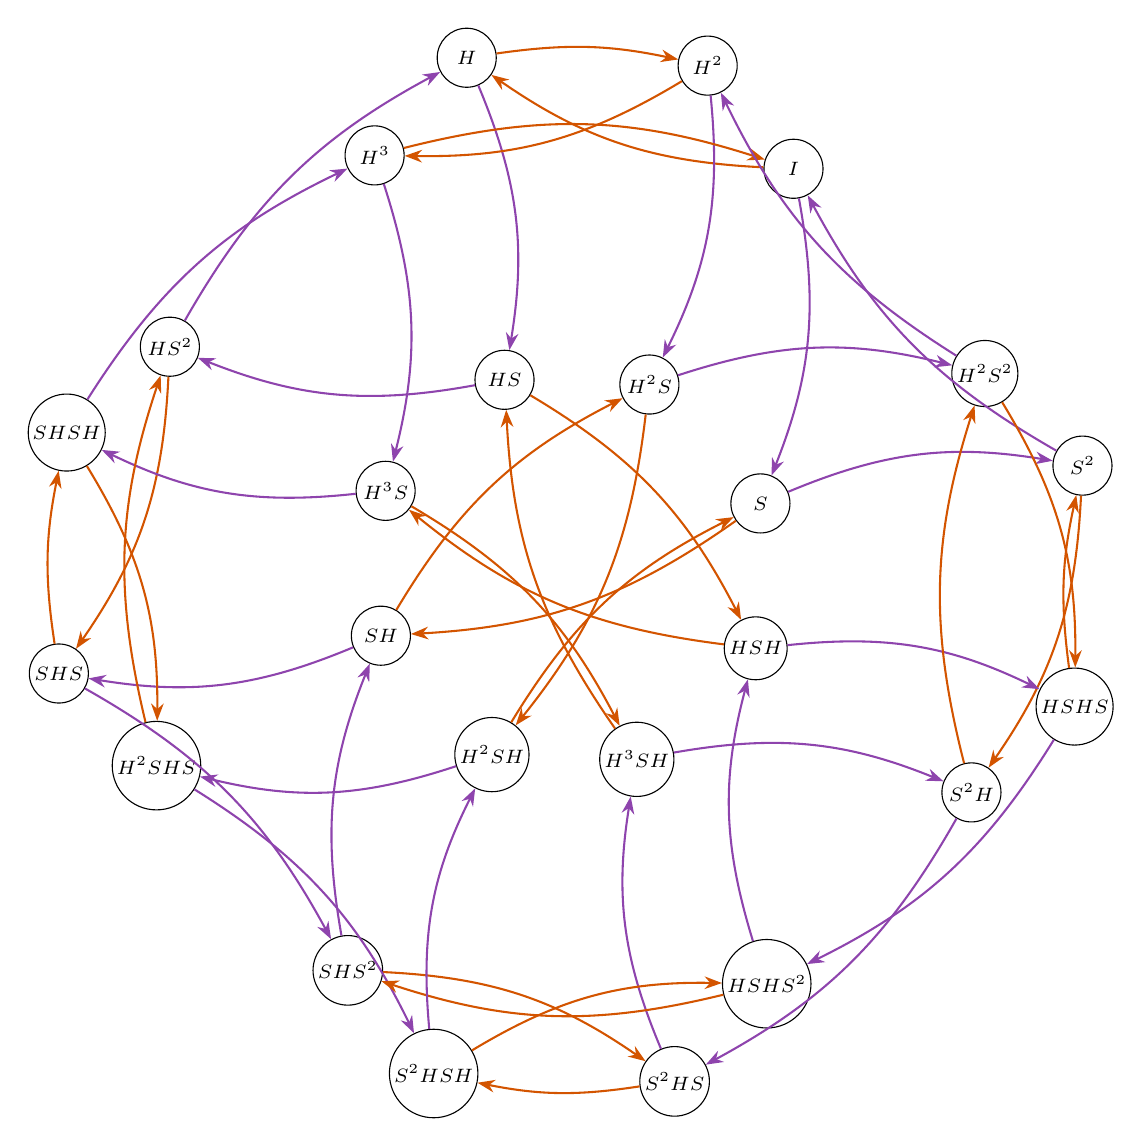
\begin{tikzpicture}[>={Stealth[length=2.2mm,width=1.6mm]},
  cnode/.style={circle,draw=black,fill=white,inner sep=1.1pt,minimum size=7.5mm,font=\scriptsize},
  Hedge/.style={->,HCol,line width=0.75pt},
  Sedge/.style={->,SwapCol,line width=0.75pt}]
  \node[cnode] (n0) at (2.83,5.09) {$I$};
  \node[cnode] (n1) at (-1.32,6.5) {$H$};
  \node[cnode] (n2) at (2.41,0.84) {$S$};
  \node[cnode] (n3) at (1.74,6.4) {$H^2$};
  \node[cnode] (n4) at (-0.84,2.41) {$HS$};
  \node[cnode] (n5) at (-2.41,-0.84) {$SH$};
  \node[cnode] (n6) at (6.5,1.32) {$S^2$};
  \node[cnode] (n7) at (-2.49,5.26) {$H^3$};
  \node[cnode] (n8) at (1.0,2.35) {$H^2S$};
  \node[cnode] (n9) at (2.35,-1.0) {$HSH$};
  \node[cnode] (n10) at (-5.09,2.83) {$HS^2$};
  \node[cnode] (n11) at (-6.5,-1.32) {$SHS$};
  \node[cnode] (n12) at (5.09,-2.83) {$S^2H$};
  \node[cnode] (n13) at (-2.35,1.0) {$H^3S$};
  \node[cnode] (n14) at (-1.0,-2.35) {$H^2SH$};
  \node[cnode] (n15) at (5.26,2.49) {$H^2S^2$};
  \node[cnode] (n16) at (6.4,-1.74) {$HSHS$};
  \node[cnode] (n17) at (-6.4,1.74) {$SHSH$};
  \node[cnode] (n18) at (-2.83,-5.09) {$SHS^2$};
  \node[cnode] (n19) at (1.32,-6.5) {$S^2HS$};
  \node[cnode] (n20) at (0.84,-2.41) {$H^3SH$};
  \node[cnode] (n21) at (-5.26,-2.49) {$H^2SHS$};
  \node[cnode] (n22) at (2.49,-5.26) {$HSHS^2$};
  \node[cnode] (n23) at (-1.74,-6.4) {$S^2HSH$};
  \draw[Hedge] (n0) to[bend left=16] (n1);
  \draw[Sedge] (n0) to[bend left=16] (n2);
  \draw[Hedge] (n1) to[bend left=10] (n3);
  \draw[Sedge] (n1) to[bend left=16] (n4);
  \draw[Hedge] (n2) to[bend left=16] (n5);
  \draw[Sedge] (n2) to[bend left=16] (n6);
  \draw[Hedge] (n3) to[bend left=16] (n7);
  \draw[Sedge] (n3) to[bend left=16] (n8);
  \draw[Hedge] (n4) to[bend left=16] (n9);
  \draw[Sedge] (n4) to[bend left=16] (n10);
  \draw[Hedge] (n5) to[bend left=16] (n8);
  \draw[Sedge] (n5) to[bend left=16] (n11);
  \draw[Hedge] (n6) to[bend left=16] (n12);
  \draw[Sedge] (n6) to[bend left=16] (n0);
  \draw[Hedge] (n7) to[bend left=16] (n0);
  \draw[Sedge] (n7) to[bend left=16] (n13);
  \draw[Hedge] (n8) to[bend left=16] (n14);
  \draw[Sedge] (n8) to[bend left=16] (n15);
  \draw[Hedge] (n9) to[bend left=16] (n13);
  \draw[Sedge] (n9) to[bend left=16] (n16);
  \draw[Hedge] (n10) to[bend left=16] (n11);
  \draw[Sedge] (n10) to[bend left=16] (n1);
  \draw[Hedge] (n11) to[bend left=10] (n17);
  \draw[Sedge] (n11) to[bend left=16] (n18);
  \draw[Hedge] (n12) to[bend left=16] (n15);
  \draw[Sedge] (n12) to[bend left=16] (n19);
  \draw[Hedge] (n13) to[bend left=16] (n20);
  \draw[Sedge] (n13) to[bend left=16] (n17);
  \draw[Hedge] (n14) to[bend left=16] (n2);
  \draw[Sedge] (n14) to[bend left=16] (n21);
  \draw[Hedge] (n15) to[bend left=16] (n16);
  \draw[Sedge] (n15) to[bend left=16] (n3);
  \draw[Hedge] (n16) to[bend left=10] (n6);
  \draw[Sedge] (n16) to[bend left=16] (n22);
  \draw[Hedge] (n17) to[bend left=16] (n21);
  \draw[Sedge] (n17) to[bend left=16] (n7);
  \draw[Hedge] (n18) to[bend left=16] (n19);
  \draw[Sedge] (n18) to[bend left=16] (n5);
  \draw[Hedge] (n19) to[bend left=10] (n23);
  \draw[Sedge] (n19) to[bend left=16] (n20);
  \draw[Hedge] (n20) to[bend left=16] (n4);
  \draw[Sedge] (n20) to[bend left=16] (n12);
  \draw[Hedge] (n21) to[bend left=16] (n10);
  \draw[Sedge] (n21) to[bend left=16] (n23);
  \draw[Hedge] (n22) to[bend left=16] (n18);
  \draw[Sedge] (n22) to[bend left=16] (n9);
  \draw[Hedge] (n23) to[bend left=16] (n22);
  \draw[Sedge] (n23) to[bend left=16] (n14);
\end{tikzpicture}
  }
  \caption{Cayley graph of the quotient $\mathcal{C}_3/\mathcal{P}_3 \cong SL(2,\mathbb{Z}_3)$. Each of the $24$ nodes is one coset representative, labeled by the word that the breadth-first traversal assigned to it, with repeated symbols written as powers. Orange arrows denote right multiplication by $H$ and purple arrows right multiplication by $S$. The $S$ arrows close into eight directed $3$-cycles and the $H$ arrows into six directed $4$-cycles, as the orders of the two generators require, and every element is reached from the identity $I$ within five steps.}
  \label{fig:cayley-c3modp3}
\end{figure*}

\paragraph{Words of the catalog.}
The catalog consists of the products $P \cdot C$, where $P = X^a Z^b$ runs over the nine Pauli operators and $C$ over the $24$ coset words. Identity factors are dropped, and the product of the two identities is the single word $I$. This gives $216$ words in the symbols $X$, $Z$, $H$, $S$ and $I$, such as $X^2Z^2S^2HSH$. A word is read as an operator product, so that its rightmost symbol acts first and its Pauli prefix last. The words contain between one and nine symbols, $5.17$ on average.

\paragraph{From a word to a circuit.}
In the baseline each symbol of a word is one primitive gate on the qutrit, and the identity element is one identity gate. Gates are never merged, so that $X^2$ is two $X$ gates and $H^3$ is three $H$ gates. In LRB-D each symbol becomes its logical circuit: $\bar{H}$ and $\bar{S}$ are the circuits of Eqs.~\eqref{eq:logical_H} and~\eqref{eq:logical_HS} (\autoref{fig: logical H}, \autoref{fig: logical S}), $\bar{X} = X_0 X_3$ and $\bar{Z} = Z_0 Z_2$ are two one-qutrit gates each, and the logical identity is one identity gate on $q_0$. Averaged over the catalog, a logical Clifford applies $16.8$ one-qutrit and $3.2$ two-qutrit gates. Because every symbol remains a separate noisy operation, the noise of a Clifford grows with the length of its word.

\paragraph{Inverses.}
For a word $C = s_1 s_2 \cdots s_\ell$ the inverse is $C^{-1} = s_\ell^{-1} \cdots s_1^{-1}$, which in time order applies $s_1^{-1}$ first and $s_\ell^{-1}$ last. The catalog stores this inverse word for each of its $216$ elements. It is written in $H^{-1}$, $S^{-1}$, $X^{-1}$ and $Z^{-1}$, has as many symbols as the forward word, and is not replaced by a shortest word. The mirror inverse looks up the stored inverse of each Clifford of the sequence and applies it like any other word. In LRB-D the inverse of a logical symbol is its logical circuit in reverse order with every gate inverted. $\bar{H}^{-1}$, for example, applies $H$ to $q_1$ and $H^{-1}$ to $q_0$, $q_2$, $q_3$ and $q_4$ and then $\mathrm{SWAP}_{2,3}$.

\paragraph{Checks.}
The catalog and all circuits are built as \texttt{sdim} circuits, with the gates of Eq.~\eqref{eq:conventions}. We checked the catalog against these conventions by converting the single-qutrit circuit of every word to its unitary matrix. The $216$ words give $216$ distinct unitaries modulo a global phase, which coincide with the closure of $\{H, S\}$ under multiplication, and every word followed by its stored inverse gives the identity up to a phase. The same unitaries reproduce the $24$ coset words of the traversal and the $48$ edges of \autoref{fig:cayley-c3modp3}.

\subsection{Qubit Catalog}
\label{app:catalog-qubit}

% from "method.tex", line 16 of the 438f6f16 mirror
% Qubit code and catalog: FoldedQubitDetectionCode and QubitCliffordLibrary (worktree qubit-lrbd-sdim140, src/lrb/code_definitions.py), FoldedQubitConventionalSitesDetectionCode (worktree conventional-sites); checks in tests/test_folded_qubit_code.py and tests/test_conventional_sites_code.py of those worktrees.
The catalog of the $24$-element single-qubit Clifford group consists of the products of the Pauli operators $I$, $X$, $Z$ and $XZ$ with the six words $I$, $H$, $S$, $HS$, $SH$ and $HSH$, with identity factors dropped as for the qutrit. Its words contain between one and five symbols, $61/24 = 2.54$ on average, and a logical Clifford of the qubit code applies $8.2$ one-qubit and $1.5$ two-qubit gates on average. Inverses and circuits follow the rules of the qutrit catalog. The encoded circuits of all $24$ words and of their inverses act on the code space as the intended single-qubit Cliffords, and in a noiseless simulation of either layout every Pauli error of weight one on a data qubit gives a nontrivial syndrome in a check round.
 % G (track hw; parked text until M3)

% Not in the sim build (CONTRACT Sec. 6; flagged for the user): the baseband-gate appendix,
% Baseband two qubit and two qutrit gate.tex, and the hardware material (results - IQM QPU.tex in the
% old tree, hardware placeholder.tex in the hw tree).

\bibliographystyle{apsrev4-2}
\bibliography{references}

\end{document}
